\section{Background Estimation}
\label{sec:bkg_estim}
Measurement of the Higgs boson mass requires the accurate modeling of the total event yield in the signal region (SR), into which events can be categorized as either \emph{signal} or \emph{background}.
These background events pass the signal event selection (Section~\ref{sec:zz_sel}) and thus spoil the purity of the signal events.
This introduces further uncertainty into the final Higgs boson mass measurement.
Therefore, it is a priority to reduce and to predict the expected number of background events, which can be split into two types: \emph{irreducible background} (IB) and \emph{reducible background} (RB) processes.

\subsection{Irreducible Background}
\label{sec:bkg_irred}
IB processes produce two \PZ bosons and each \PZ subsequently decays into two prompt leptons (leptons that emerge directly from the primary vertex).
This reliably produces a \fourl final state, whose prompt leptons are typically reconstructed as four leptons that pass tight selection (\emph{PTS leptons}), as defined in Sections~\ref{sec:el_sel} and~\ref{sec:mu_sel}.
The IB event then looks indistinguishable from the 4 PTS lepton of the \emph{signal} process and cannot be reduced;
Thus, throwing away IB process could mean throwing away a signal event.
Since IB events cannot be completely eliminated---or \emph{reduced}---from the SR, they are given the name \emph{irreducible} backgrounds.
The two IBs for this analysis are:
\begin{itemize}
    \item \ggzzfourl (gluon-gluon fusion),
    \item \qqzzfourl (quark-antiquark annihilation).
\end{itemize}

\subsection{Reducible Background}
\label{sec:redbkg}
While IB processes produce 4 prompt leptons, RB processes produce varying numbers of prompt and nonprompt leptons.
Nonprompt leptons emerge from 3 main sources:
\begin{itemize}
    \item misidentifying light-flavor hadrons (\eg, $\pi^{\pm}$) as leptons,
    \item heavy-flavor hadrons that decay mid-flight into leptons,
    \item and the asymmetric conversion of photons into electrons.
\end{itemize}

This analysis is tailored to efficiently reconstruct prompt(nonprompt) leptons as PTS(FTS) leptons.
Ideally, the SR would contain only the events with 4 prompt leptons, which would always be tagged as 4 PTS leptons.
However, sometimes a truly nonprompt lepton is misidentified as a PTS lepton (sometimes called a \emph{fake lepton}), depending on the kinematic properties of the lepton.
This misidentification rate ($f$, sometimes called the \emph{fake rate}) is due to imperfect detector performance, inefficiencies in reconstruction, and the specific choice of lepton selections used in the analysis.

If an event produces prompt and nonprompt leptons but is reconstructed as 4 PTS leptons (a 4P event), then it contaminates the SR.
These processes constitute the RB processes (sometimes called ``\ZplusX'').
Examples of RB processes for this analysis include:
\begin{itemize}
	\item \Zplusjets (yields 2 prompt leptons)
	\item \ttbarplusjets (yields 2 prompt leptons)
	\item \WZplusjets (yields 3 prompt leptons)
	\item $\ZZ/Zgammastar + \text{jets}$ (yields 4 prompt leptons).
\end{itemize}
The careful estimation of these RB contributions to the 4P region is necessary for the precise measurement of the Higgs boson mass.

\subsubsection{OS Method}
% \label{sec:os_method}
The goal of the OS Method is to estimate the number of opposite-sign same-flavor (OSSF) \fourl events produced by RB process that ``contaminate'' the 4P region $\left( \nfourPRB \right)$, given by Eq.~\ref{eqn:rbe_formula_final}.
% Since the $4\ell$ final state of the signal process consists of 2 pairs of OSSF leptons, the method is called the \emph{OS Method}.
However, the typical approach of using simulated samples does not model RB well, since RB processes (\eg, \Zplusjets) rely on higher-order effects like jet modelling which are not yet accurately simulated.
Instead, a data-driven approach is used.

The logic of the OS Method is to study events in data that are similar to, but not exactly the same as, those found in the 4P region.
Thus, events in data are sorted into 2 control regions (CRs), both of which are orthogonal to the 4P region and to each other:
\begin{itemize}
	\item the \emph{3P1F} CR (built from 3 PTS and 1 FTS leptons)
	\item the \emph{2P2F} CR (built from 2 PTS and 2 FTS leptons).
\end{itemize}
The event selection for the 2P2F and 3P1F CRs is almost identical to that of the SR (Section~\ref{sec:zz_sel}),
except that the FTS lepton(s) are required to build the \Ztwo.
The events that contribute mostly to the 2P2F(3P1F) CR are those that produce 2(3) prompt and 2(1) nonprompt leptons and are called \emph{2pr}(\emph{3pr}) events.
Similarly, the events that contribute mostly to the 4P SR are those that produce 4 prompt leptons and are called \emph{4pr} events.

The final formula for \nfourPRB is obtained by first supposing that event $k$ is a 2pr event and contributes to the 2P2F CR an event weight of $\wgttwoprompttotwoPtwoF^k$.
This weight is built from $\hat{w}^k$, which is the product of analysis weights (pileup, L1 pre-firing, \etc), and the reconstruction efficiencies ($\epsilon$) of each lepton ($\ell_n$):
\begin{equation}
	\label{eqn:wt_2prto2p2f}
	\wgttwoprompttotwoPtwoF^k = \hat{w}^k \cdot \effprpass(\ell_1^k) \cdot \effprpass(\ell_2^k) \cdot \effnpfail(\ell_3^k) \cdot \effnpfail(\ell_4^k),
\end{equation}
where the superscript of $\epsilon$ indicates the lepton promptness (pr = prompt, np = nonprompt),
the subscript indicates the lepton tightness status (P = PTS, F = FTS).
To simplify the equations that follow, $\hat{w}^k$ is set to unity.
%  \effprpass(\ell_1^k) is the efficiency of reconstructing $\ell_1$ from event $k$ as a \mathbf{P}TS lepton
% and \effnpfail(\ell_3^k) is the efficiency of reconstructing $\ell_3$ from event $k$ as a \mathbf{F}TS lepton
% where $\epsilon^{\mathrm{pr|np}}_{\mathrm{P|F}}$ is the efficiency of reconstructing a prompt/nonprompt lepton passing/failing tight selections.
If the reconstruction efficiencies of a particular category are the same for all $j$ leptons across all $k$ events $\left( \eg, ~ \effprpass(\ell_j^k) \equiv \effprpass \right)$, then Eq.~\ref{eqn:wt_2prto2p2f} reduces to:
\begin{equation}
	\label{eqn:wt_2prto2p2f_simp}
	\wgttwoprompttotwoPtwoF^k = 
	\left( \effprpass \right)^2 
	\left( \effnpfail \right)^2.
\end{equation}

Although a 2pr event mostly contributes to the 2P2F CR, a nonprompt lepton may be misidentified as a PTS lepton, depending on \effnppass.
Such an event would then fall into the 3P1F CR and, allowing for only one nonprompt PTS lepton at a time, contributes an effective weight of
\begin{align}
	\label{eqn:wt_2prto3p1f}
	\wgttwoprompttothreePoneF^k
	&= \left( \effprpass \right)^2 
	\left[
		\effnppass(\ell_1^k) \cdot \effnpfail(\ell_2^k) + \effnpfail(\ell_1^k) \cdot \effnppass(\ell_2^k)
	\right]
	\notag
	\\
	&= \left( \effprpass \right)^2
	\left[
		2 \effnppass \effnpfail
	\right].
\end{align}
Using the fact that a (non)prompt lepton is exclusively either PTS or FTS
$\left( \epsilon^\text{pr(np)}_\text{P} + \epsilon^\text{pr(np)}_\text{F} = 1 \right)$,
% \begin{equation*}
% 	\epsilon^\mathrm{pr(np)}_\mathrm{P} + \epsilon^\mathrm{pr(np)}_\mathrm{F} = 1,
% \end{equation*}
while recognizing that $\effnppass \equiv f$ (Section~\ref{sec:redbkg}) and defining $\effprpass \equiv \epsilon$,
allows Eq.~\ref{eqn:wt_2prto3p1f} to be written as
\begin{equation}
	\label{eqn:wt_2prto3p1f_simp}
	\wgttwoprompttothreePoneF^k = 2 \epsilon^2 f (1-f).
\end{equation}
The prediction of Eq.~\ref{eqn:wt_2prto3p1f_simp} can be seen in Figures~\ref{cr_plots_3p1f_2016prevfp}--\ref{cr_plots_3p1f_2018} for 2016--2018 UL data.

Even more rarely, both nonprompt leptons from a 2pr event may be misidentified as PTS leptons.
In this case, event $k$ contributes to the 4P region an effective weight of
\begin{equation}
	\label{eqn:wt_2prto4p}
	\wgttwoprompttofourP^k = \epsilon^2 f^2,
\end{equation}
where it is assumed that both leptons have the same misidentification rate.
Similar equations can be derived for the contributions of a 3pr event to the 3P1F CR and to the 4P region:
\begin{align}
	\label{eqn:wt_3prto3p1f}
	\wgtthreeprompttothreePoneF^k &= \epsilon^3 \left( 1-f \right)
	\\
	\label{eqn:wt_3prto4p}
	\wgtthreeprompttofourP^k &= \epsilon^3 f.
\end{align}
Since a 3pr event needs only 1 nonprompt PTS lepton to be included in the 4P region (therefore, carrying only 1 factor of $f$), a 3pr event tends to contribute more weight to 4P than does a 2pr event (which carries $f^2$).

If the total number of 2pr, 3pr, and 4pr events is \xtwoprompt, \xthreeprompt, and \xfourprompt, respectively, then Figure~\ref{fig:prompt_to_crs} shows how the weight of a single event, derived in the previous equations (and others forthcoming), from each category contributes to the final yield of each CR $\left( \ntwoPtwoF, \nthreePoneF \right)$ and of the SR $\left( \nfourP \right)$.
% \begin{figure}[!htbp]
% 	\begin{center}
% 		\begin{tikzpicture}
% 			\node (X2pr) {\xtwoprompt};
% 			\node[right=4cm of X2pr] (X3pr) {\xthreeprompt};
% 			\node[right=4cm of X3pr] (X4pr) {\xfourprompt};
% 			\node[below=2cm of X2pr] (N2p) {\ntwoPtwoF};
% 			\node[below=2cm of X3pr] (N3p) {\nthreePoneF};
% 			\node[below=2cm of X4pr] (N4p) {\nfourP};
% 			% \draw[-latex] (X3pr) -- (N4p) node[xshift=2cm,yshift=1cm,rotate=45] {some words};
% 			% \draw[-latex] (X3pr) -- (N4p) node[midway,above,rotate=45] {words};
% 			% \draw[-latex] (X3pr) -- (N4p) node[sloped, anchor=center] {words};
% 		\end{tikzpicture}
% 		\caption{
% 			Each category of prompt processes contribute an effective event weight $\left( w^k \right)$ The total number of events that yield 2/3/4 prompt leptons each con
% 			}
% 		\label{fig:prompt_to_crs}
% 	\end{center}
% \end{figure}
It is then straightforward to evaluate the expected number of RB 4P events:
\begin{align}
	\label{eqn:n4p_x2x3}
	\nfourPRB
	&= \sum_{k=1}^{\xtwoprompt} \wgttwoprompttofourP^k + \sum_{m=1}^{\xthreeprompt} \wgtthreeprompttofourP^m
	\notag
	\\
	&= \sum_{k=1}^{\xtwoprompt} \epsilon^2 f^2 + \sum_{m=1}^{\xthreeprompt} \epsilon^3 f
	\notag
	\\
	&= f^2 \epsilon^2 \xtwoprompt + f \epsilon^3 \xthreeprompt,
\end{align}
where only the quantities $f$ and $\epsilon$ are known, so \xtwoprompt and \xthreeprompt must be estimated.
This is achieved by relating \xtwoprompt to \ntwoPtwoF using Eq.~\ref{eqn:wt_2prto2p2f_simp} across all 2pr events:
% If the total number of true 2pr events is \xtwoprompt, then the expected number of 2P2F events $\left( \ntwoPtwoF \right)$ is obtained via Eq.:
\begin{align}
	\label{eqn:n2p2f_x2}
	\ntwoPtwoF
	&= \sum_{k=1}^{\xtwoprompt} \wgttwoprompttotwoPtwoF^k
	\notag
	\\
	% &= \sum_{k=1}^{\xtwoprompt} \epsilon^2 \left( \effnpfail \right)^2
	% \\
	&= \sum_{k=1}^{\xtwoprompt} \epsilon^2 \left( 1-f \right)^2
	\notag
	\\
	&= \left( 1-f \right)^2 \epsilon^2 \xtwoprompt
	% \\
	% \implies \xtwoprompt &= \frac{ \ntwoPtwoF }{ \epsilon^2 \left( 1-f \right)^2 }
\end{align}

\begin{figure}[!htbp]
	\begin{center}
		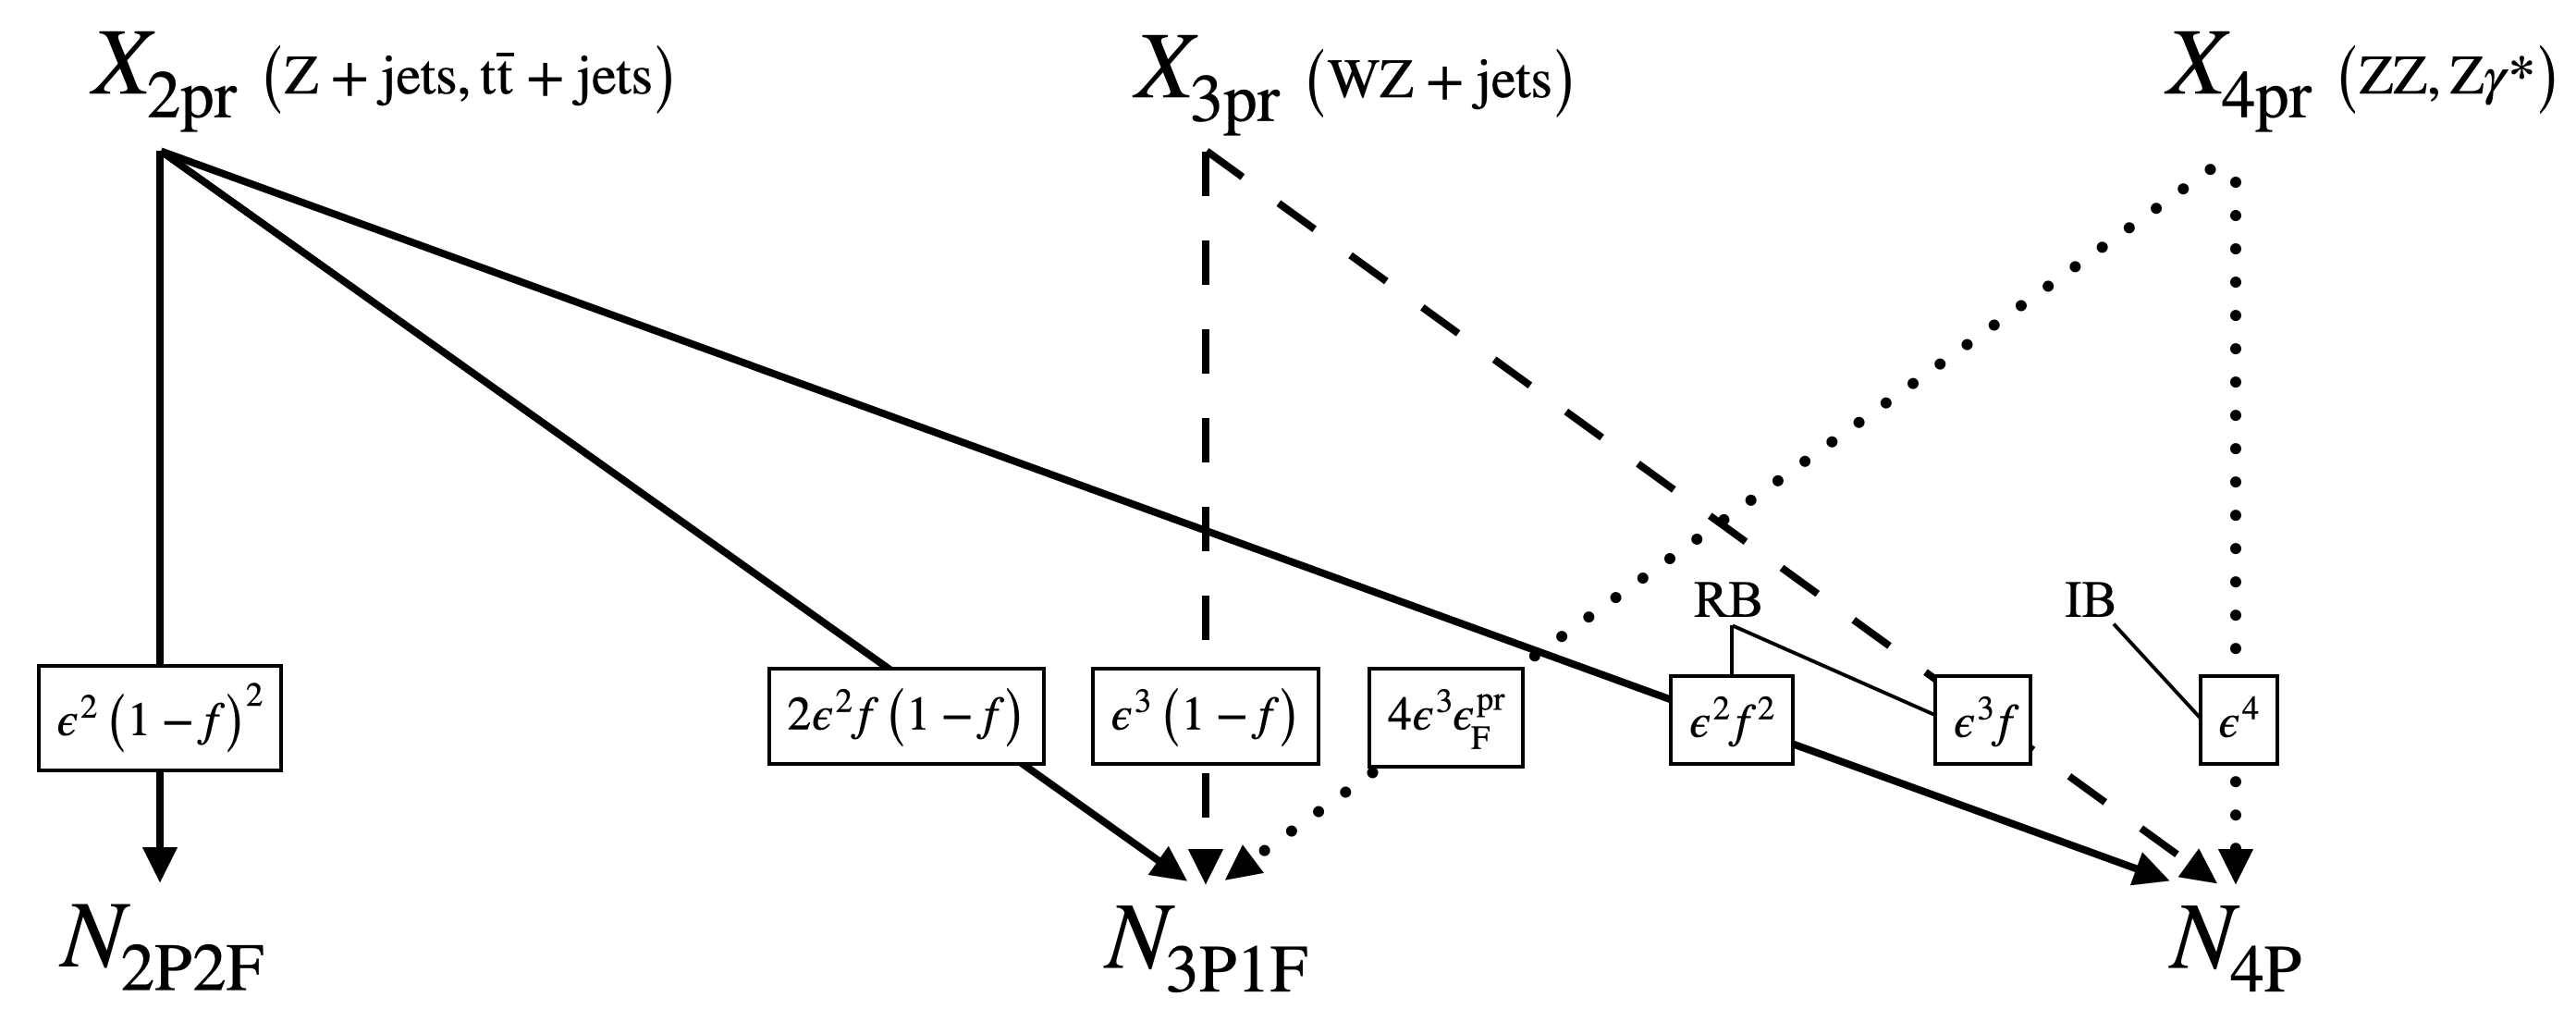
\includegraphics[width=0.95\textwidth]{figures/higgsmassmeas/redbkg/promptwgts_to_CRSR.png}
		\caption{
			Contributions of per-event weights (boxed values) of various $n$-prompt-lepton processes ($X_{n\text{pr}}$, in parentheses) to the total numbers of events in the observed control regions $\left( \ntwoPtwoF, \nthreePoneF \right)$ and signal region $\left( \nfourP \right)$.
			The labels ``IB'' and ``RB'' indicate those contributions which comprise the irreducible and reducible backgrounds, respectively.
		}
		\label{fig:prompt_to_crs}
	\end{center}
\end{figure}

The strategy to relate \xthreeprompt to \nthreePoneF is not as straightforward as relating \xtwoprompt to \ntwoPtwoF,
since two other sources also contribute to the 3P1F CR (as shown in Figure~\ref{fig:prompt_to_crs}):
\begin{itemize}
	\item A 2pr RB process can yield one nonprompt PTS lepton (via Eq.~\ref{eqn:wt_2prto3p1f_simp}).
	\item A 4-prompt IB process (\qqggzzfourl, ``\ZZ'') can yield one FTS lepton.
\end{itemize}
The second of these is well estimated from simulation, since \ZZ produces 4 prompt leptons.
If the total number of simulated \ZZ events is \xfourpromptzz, then event $k$ belonging to these events contributes to the 3P1F CR an effective weight of
\begin{equation}
	\label{eqn:wt_4przzto3p1f}
	\wgtfourpromptzztothreePoneF^k = 4 \epsilon^3 \effprfail,
\end{equation}
which accounts for any of the 4 prompt leptons to be reconstructed as a FTS lepton while the others are PTS leptons.
Incorporating Eqs.~\ref{eqn:wt_2prto3p1f_simp},~\ref{eqn:wt_3prto3p1f}, and~\ref{eqn:wt_4przzto3p1f} for all events relates \xthreeprompt to \nthreePoneF:
\begin{align}
	\label{eqn:n3p1f_x3}
	\nthreePoneF
	&= \sum_{j=1}^{\xthreeprompt} \wgtthreeprompttothreePoneF^j + \sum_{k=1}^{\xtwoprompt} \wgttwoprompttothreePoneF^k + \sum_{m=1}^{\xfourpromptzz} \wgtfourpromptzztothreePoneF^m
	\notag
	\\
	&= \sum_{j=1}^{\xthreeprompt} \epsilon^3 (1-f) + \sum_{k=1}^{\xtwoprompt} 2 \epsilon^2 f (1-f) + \sum_{m=1}^{\xfourpromptzz} 4 \epsilon^3 \effprfail
	\notag
	\\
	&= (1-f) \epsilon^3 \xthreeprompt + 2 f (1-f) \epsilon^2 \xtwoprompt + 4 \epsilon^3 \effprfail \xfourpromptzz
	\notag
	\\
	&= (1-f) \epsilon^3 \xthreeprompt + 2 f (1-f) \epsilon^2 \xtwoprompt + \nthreePoneFzz,
\end{align}
where \nthreePoneFzz is simply the raw (integer) number of \ZZ events that pass 3P1F selections, obtained directly from simulation.

At this point, \nfourPRB can be isolated by combining Eqs.~\ref{eqn:n4p_x2x3},~\ref{eqn:n2p2f_x2}, and~\ref{eqn:n3p1f_x3}:
% (the substitutions $A = \epsilon^2 X_2, B = \epsilon^3 X_3$ are quite useful)
\begin{equation}
	\label{eqn:rbe_formula}
	\nfourPRB =
	\left( \frac{f}{1-f} \right) \nthreePoneF^{\text{Data}} -
	\left( \frac{f}{1-f} \right)^2 \ntwoPtwoF^{\text{Data}} - 
	\left( \frac{f}{1-f} \right) \nthreePoneFzz.
\end{equation}
Thus, Eq.~\ref{eqn:rbe_formula} estimates the RB contribution to the 4P region by using a single lepton misidentification rate to reweight the raw yields of events found in the 3P1F and 2P2F CRs of data, and also the 3P1F CR of \ZZ.

It should be mentioned that the above formula was derived assuming that the per event analysis weights were set to unity $\left( \hat{w}^k = 1 \right)$ before being scaled by the misidentification rates.
It was also assumed that $f$ is a constant, for all nonprompt leptons misidentified as PTS leptons across all events, which is not the case as is shown in Figures~\ref{fr_plots_el} and~\ref{fr_plots_mu}.
Thus, an extension of Eq.~\ref{eqn:rbe_formula} can be formed by assigning misidentification rates that depend on the kinematical variables per lepton,
by restoring the analysis weights per event,
and by summing over the total number of raw yields per CR:
\begin{equation}
	\label{eqn:rbe_formula_final}
	\nfourPRB =
	  \sum_{i=1}^{N_{\text{3P1F}}^\text{Data}} \hat{w}^i \frac{f_i}{1 - f_i}
	- \sum_{j=1}^{N_{\text{2P2F}}^\text{Data}} \hat{w}^j \frac{f_{1,j}}{1 - f_{1,j}}\frac{f_{2,j}}{1 - f_{2,j}}
	- \sum_{k=1}^{N_{\text{3P1F}}^{\ZZ}} \hat{w}^{k}_{\ZZ} \frac{f_k}{1 - f_k},
\end{equation}
where $f_{1,j}$ and $f_{2,j}$ are the misidentification rates of the first and second FTS leptons, respectively, found in the $j^{\text{th}}$ 2P2F event
and $\hat{w}^k_{\ZZ}$ accounts for the differential QCD and electroweak $K$ factors defined in Section~\ref{sec:bkg_irred}.
% The plots in \figurename~\ref{FINAL RBE PLOTS} make use of Eq.~\ref{eqn:rbe_formula_final}.
\begin{figure}[!htbp]
	\begin{center}
		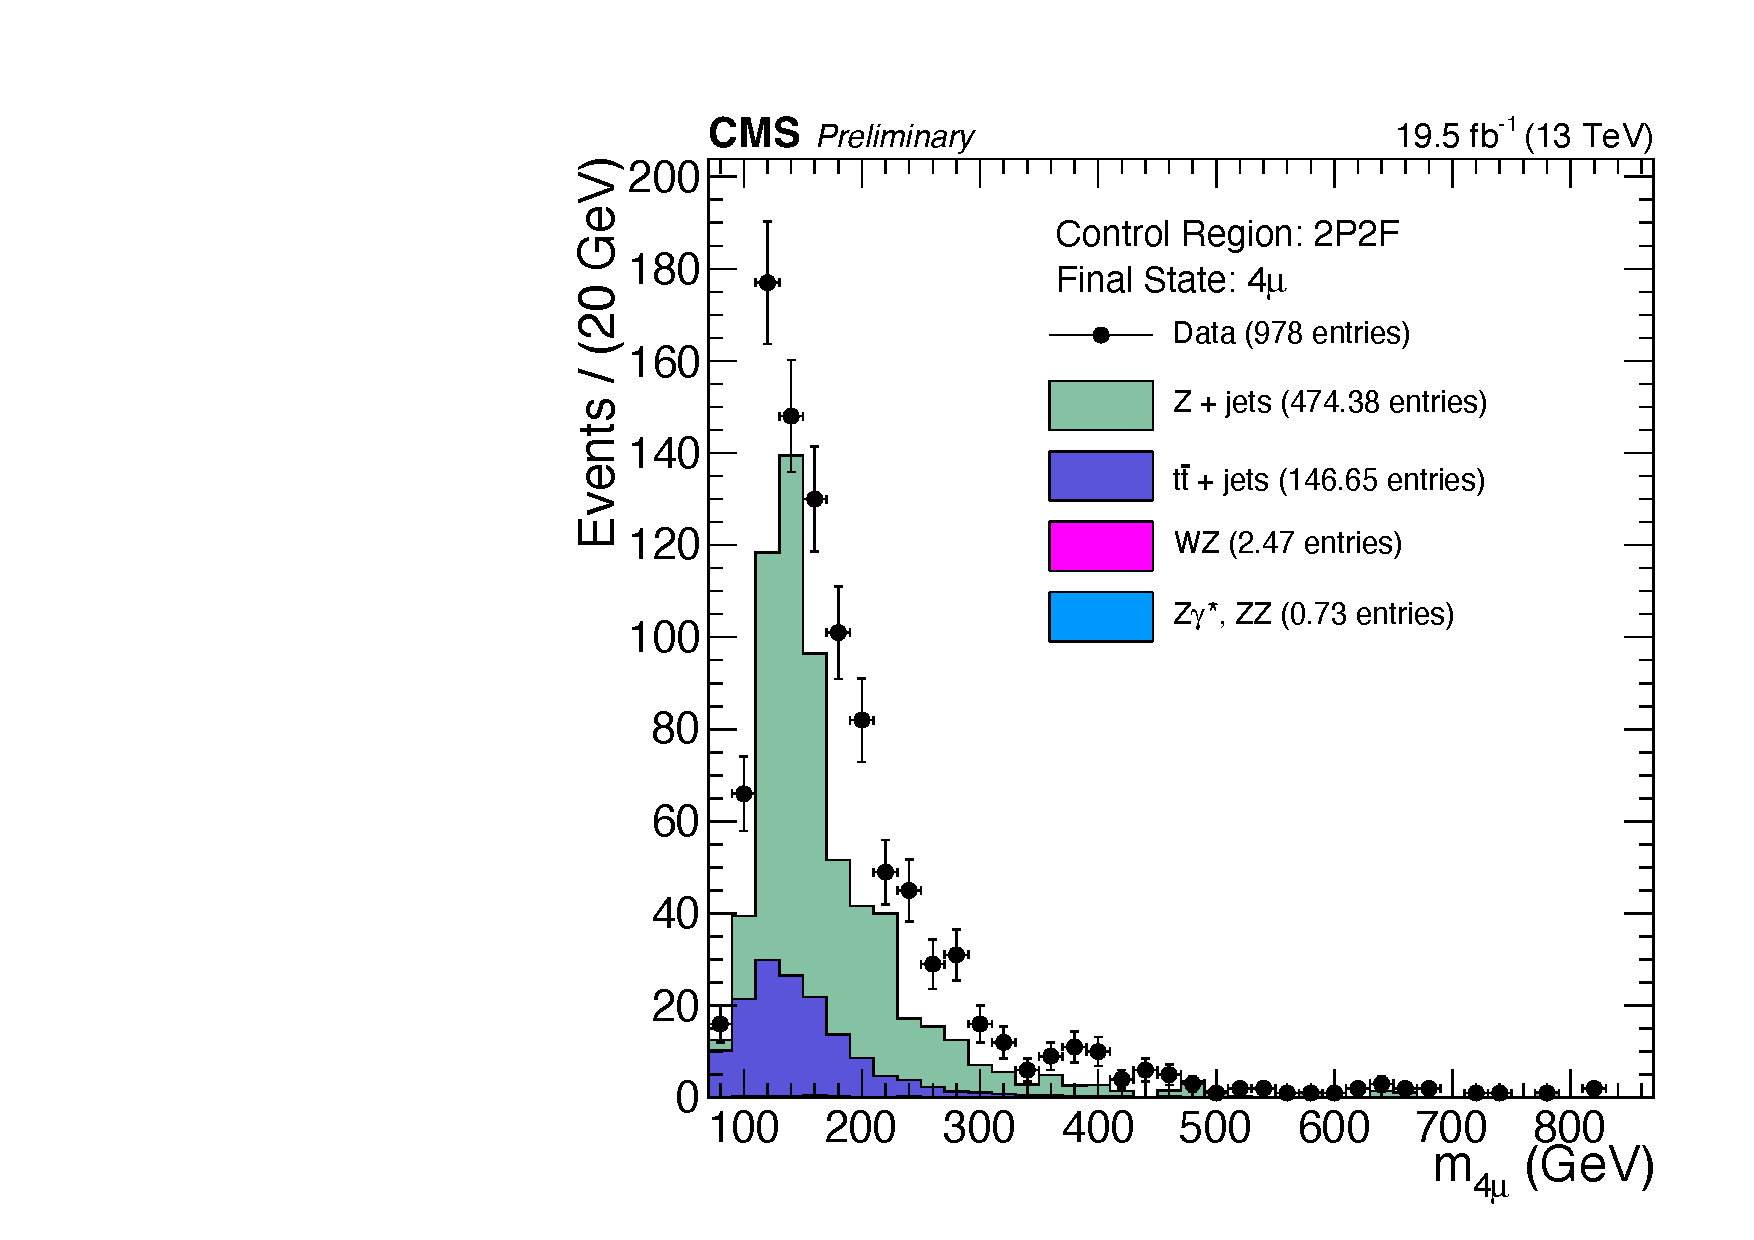
\includegraphics[width=0.48\textwidth]{figures/higgsmassmeas/redbkg/cr/UL2016preVFP_CR_2P2F_4mu.pdf}
		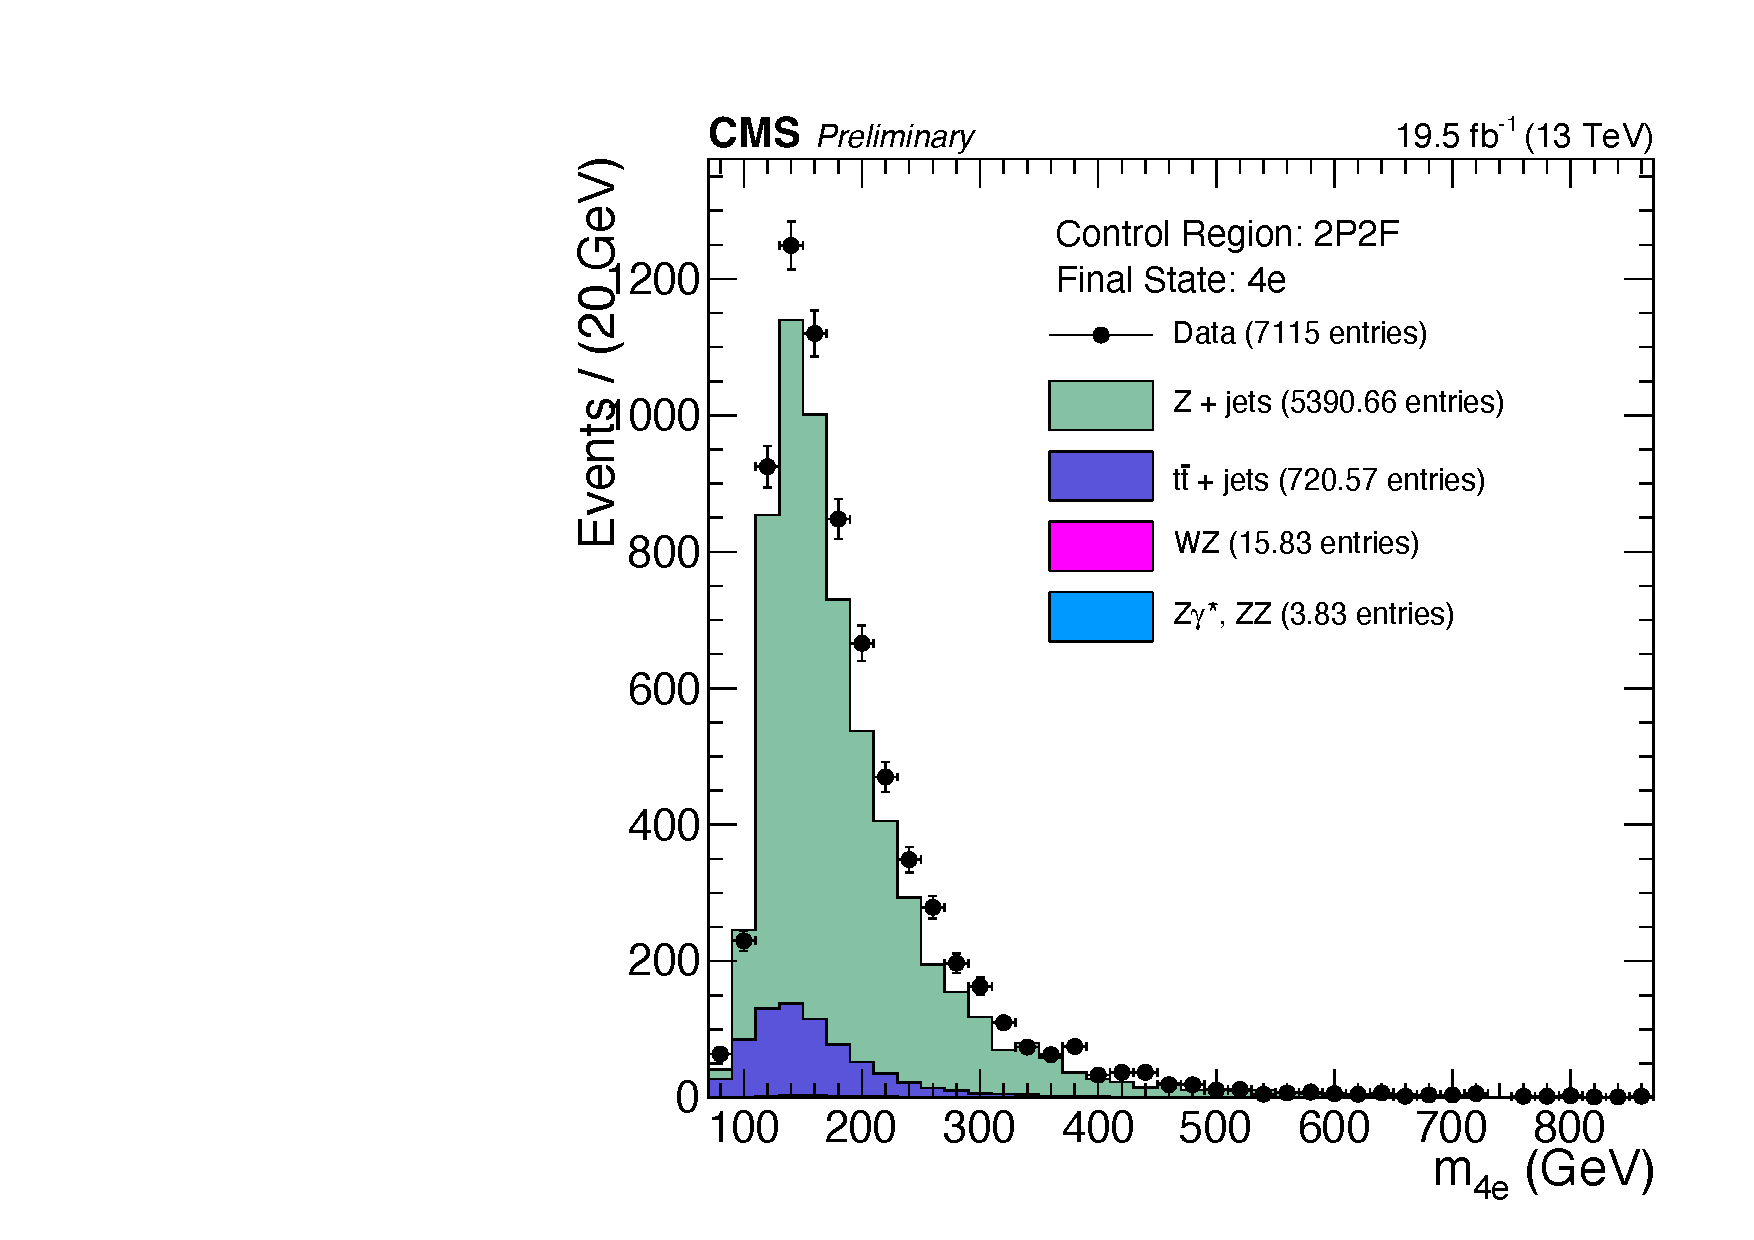
\includegraphics[width=0.48\textwidth]{figures/higgsmassmeas/redbkg/cr/UL2016preVFP_CR_2P2F_4e.pdf}
		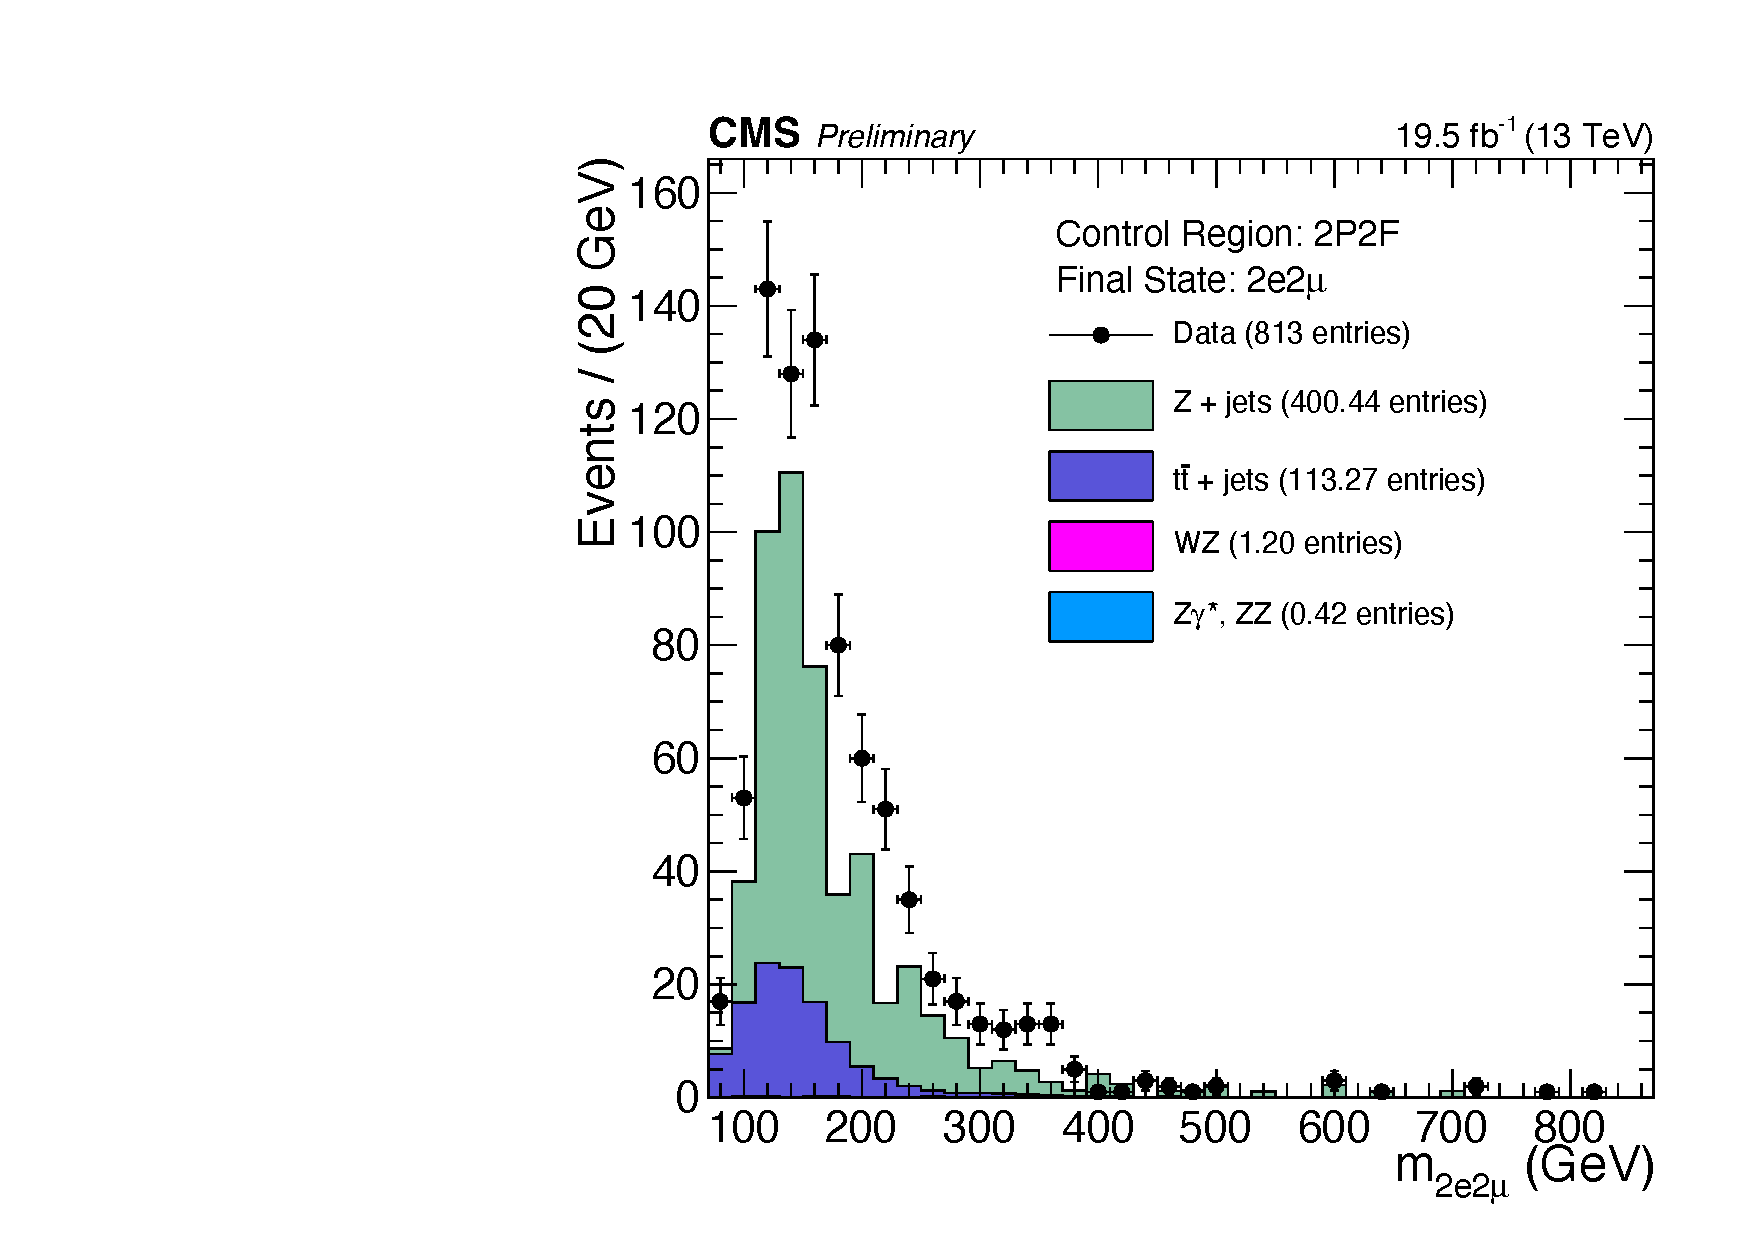
\includegraphics[width=0.48\textwidth]{figures/higgsmassmeas/redbkg/cr/UL2016preVFP_CR_2P2F_2e2mu.pdf}
		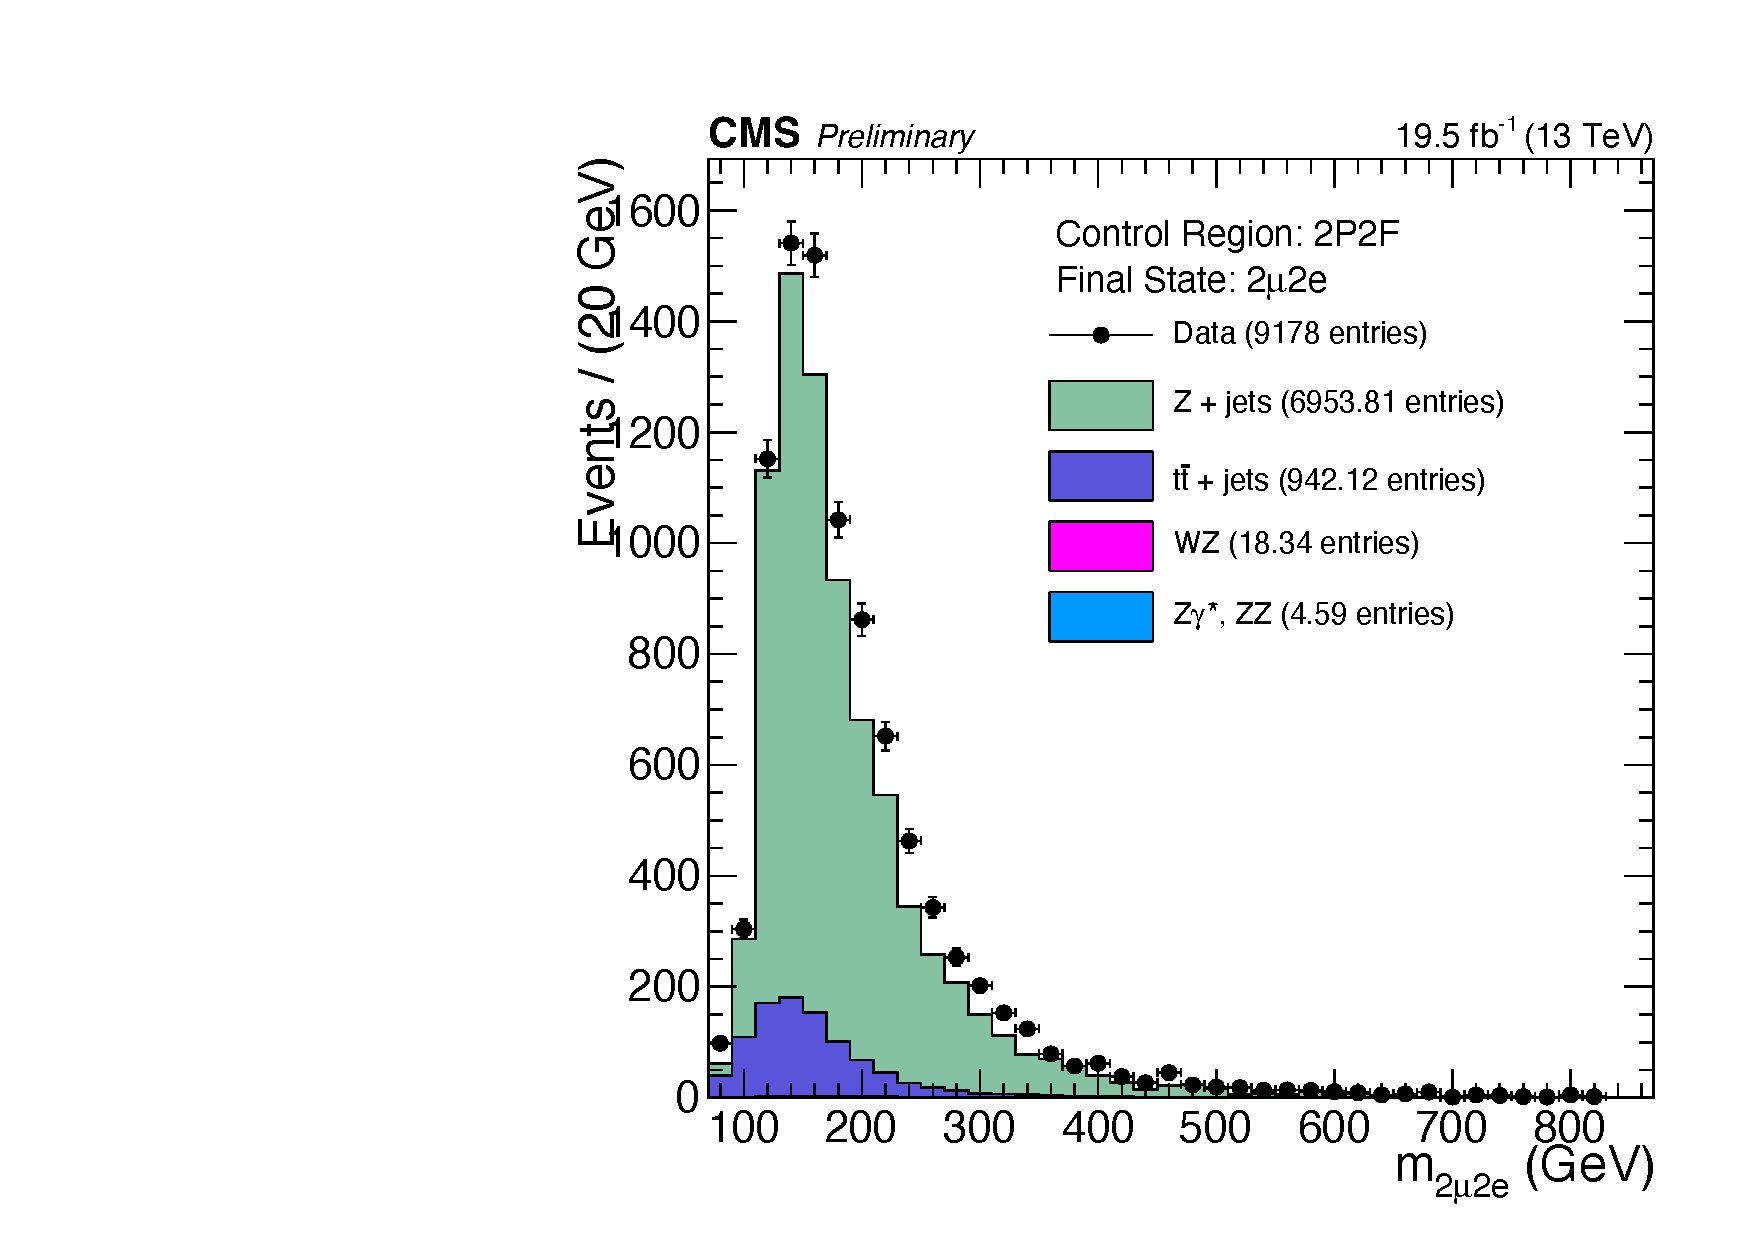
\includegraphics[width=0.48\textwidth]{figures/higgsmassmeas/redbkg/cr/UL2016preVFP_CR_2P2F_2mu2e.pdf}
		\caption{
			Events from 2016 pre-VFP UL data that pass 2P2F CR selections (black markers) 
			are compared to the stacked 2P2F distributions of simulated samples
			(\Zplusjets, \ttbarplusjets, \WZ, \ZZ, \Zgammastar).
			The results are split into the $4\ell$ final states:
            $4\mu$ (top left), 4e (top right), 2e2$\mu$ (bottom left), 2$\mu$2e (bottom right).
        }
		\label{cr_plots_2p2f_2016prevfp}
	\end{center}
\end{figure}
\begin{figure}[!htbp]
	\begin{center}
		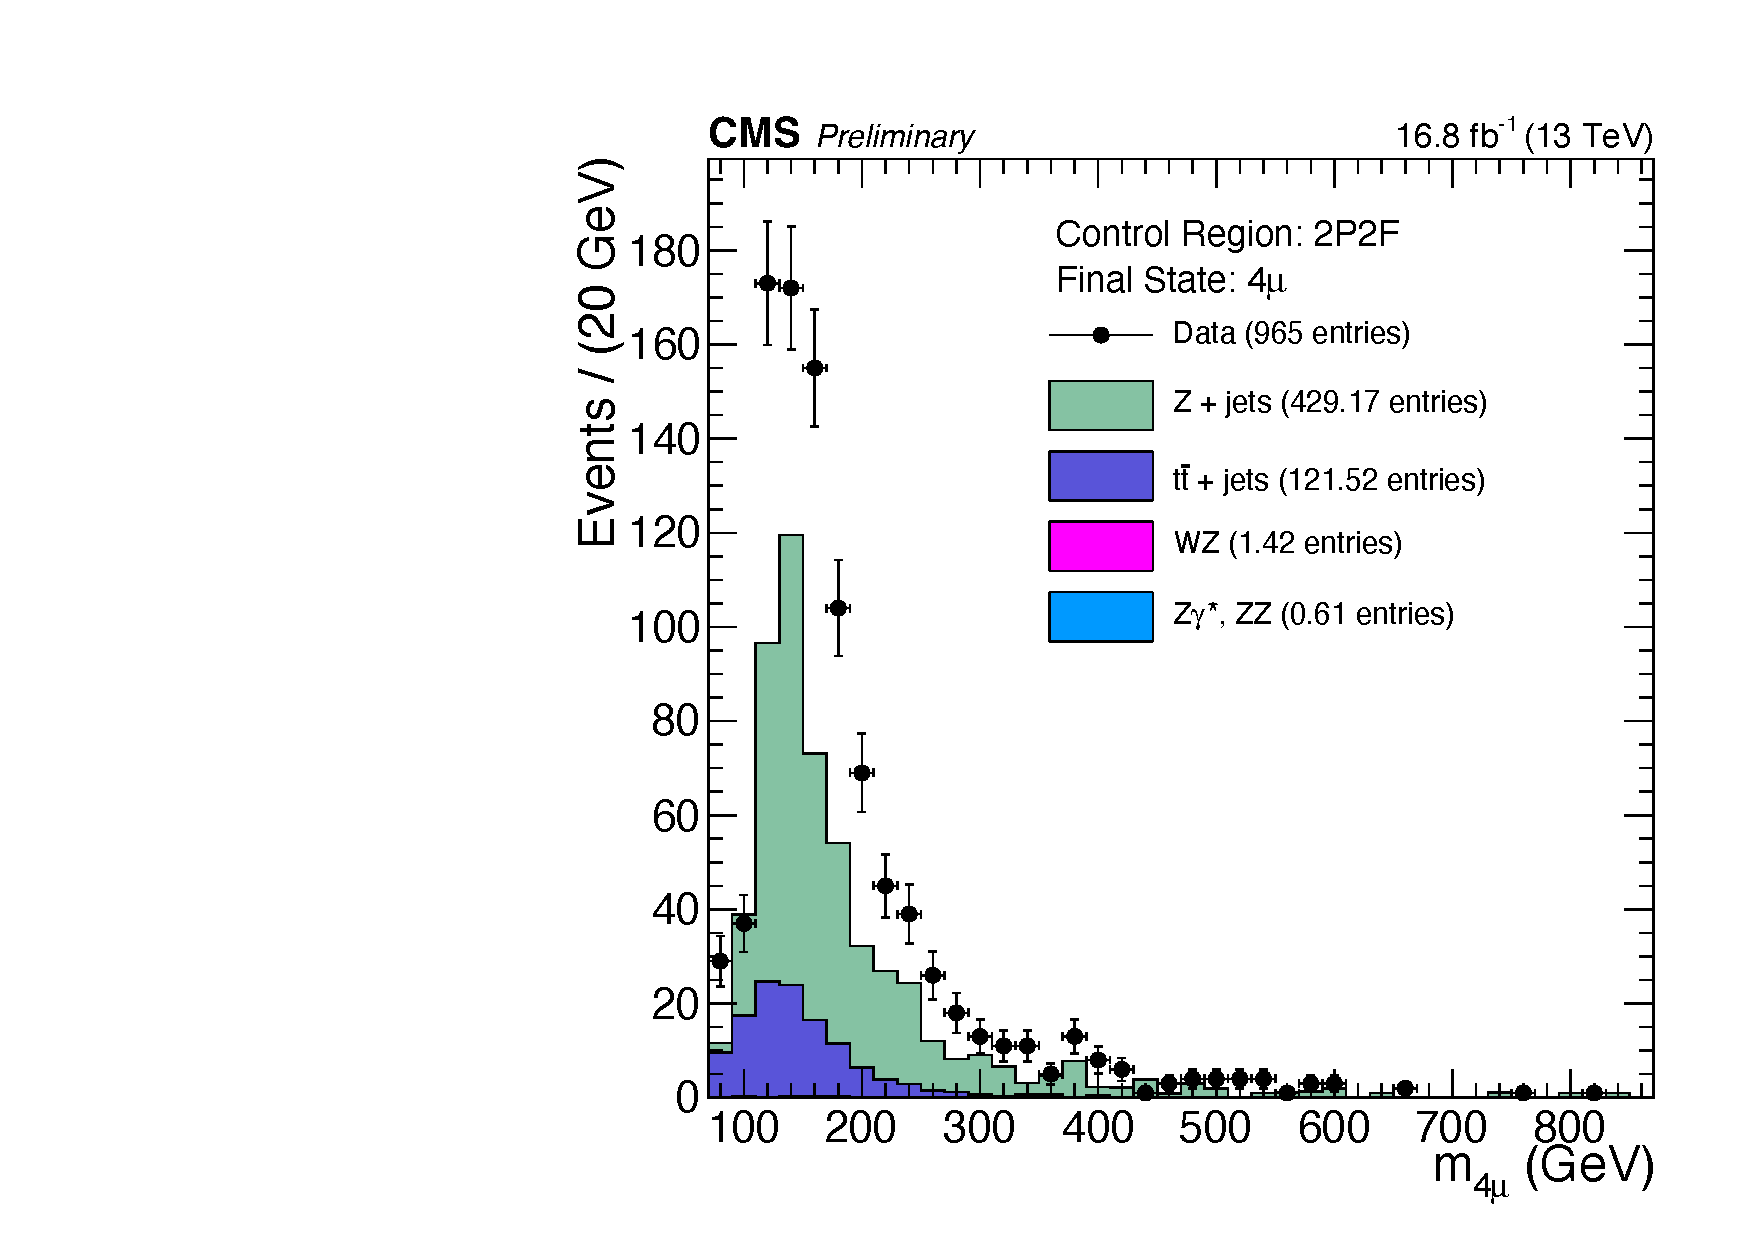
\includegraphics[width=0.48\textwidth]{figures/higgsmassmeas/redbkg/cr/UL2016postVFP_CR_2P2F_4mu.pdf}
		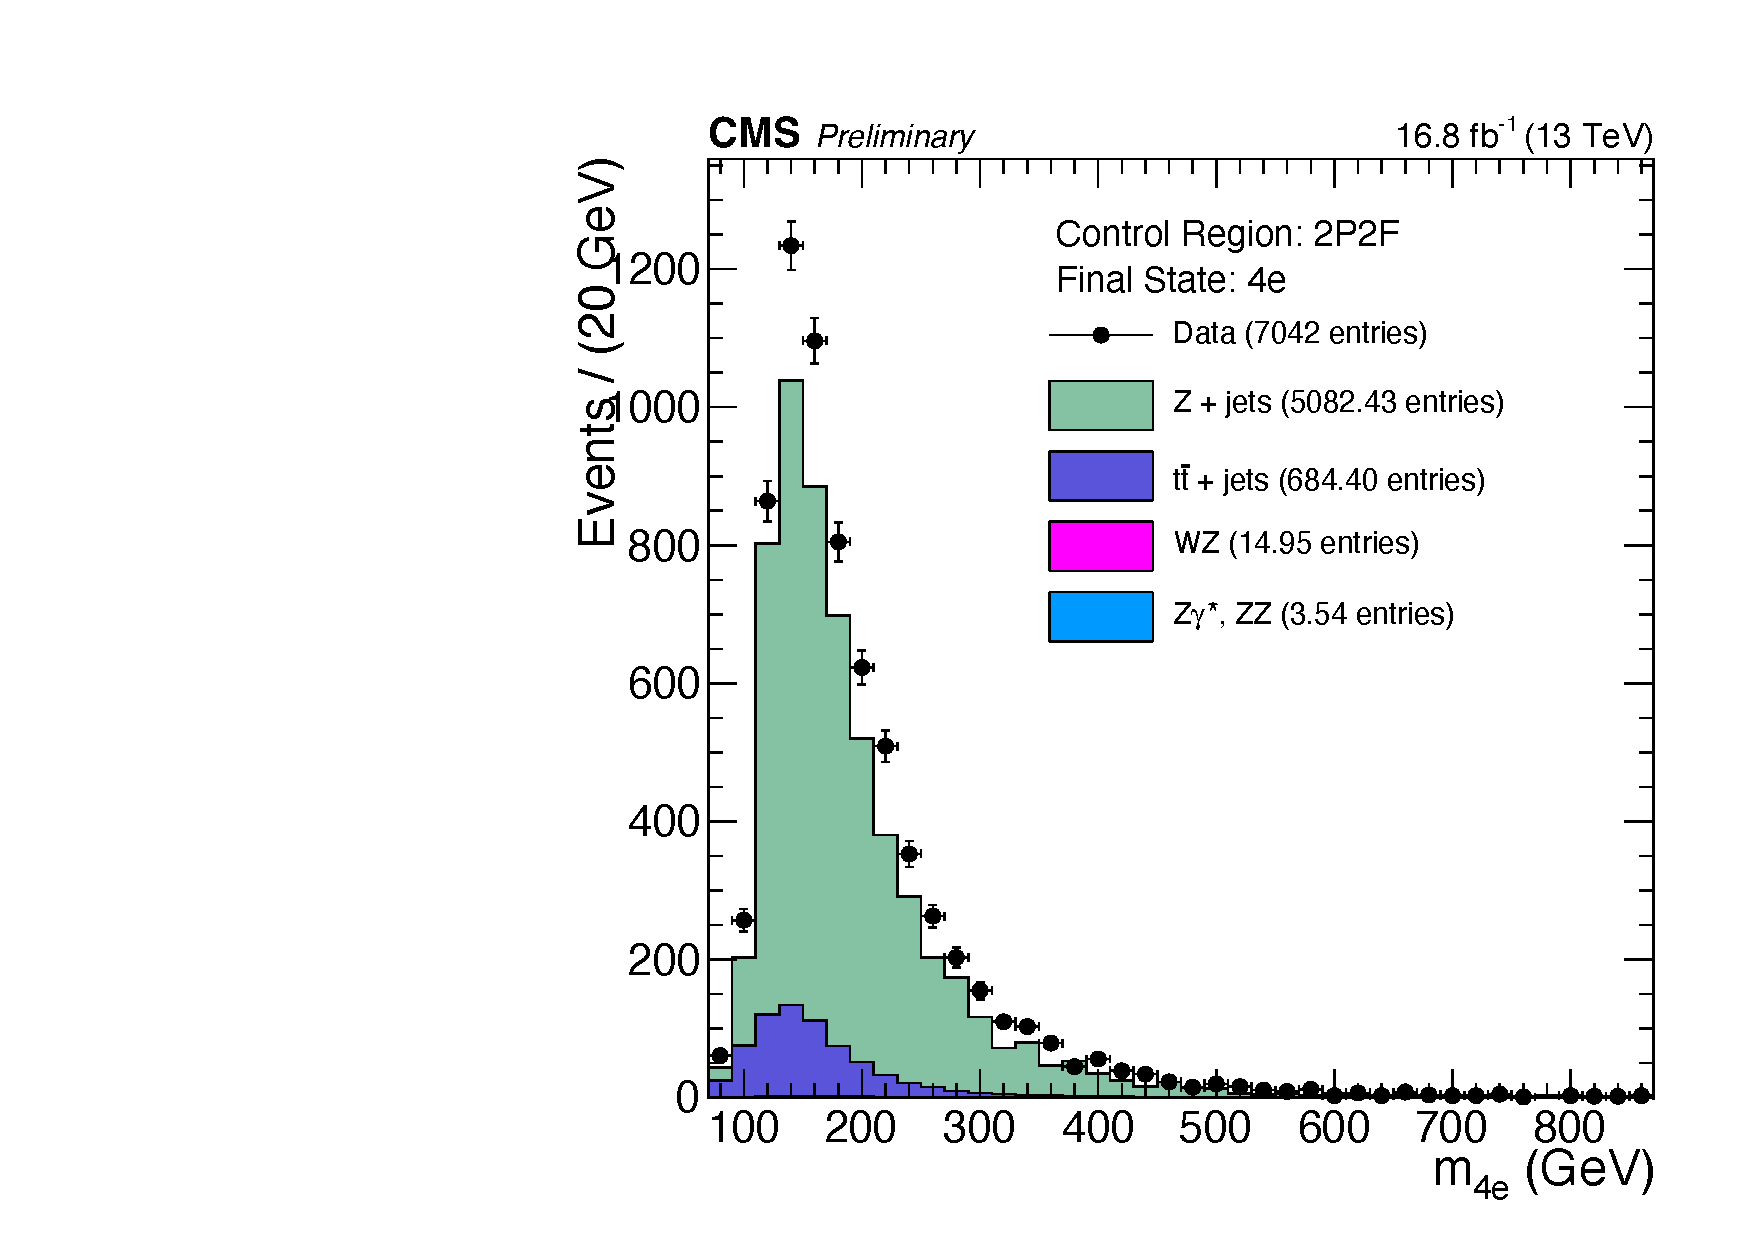
\includegraphics[width=0.48\textwidth]{figures/higgsmassmeas/redbkg/cr/UL2016postVFP_CR_2P2F_4e.pdf}
		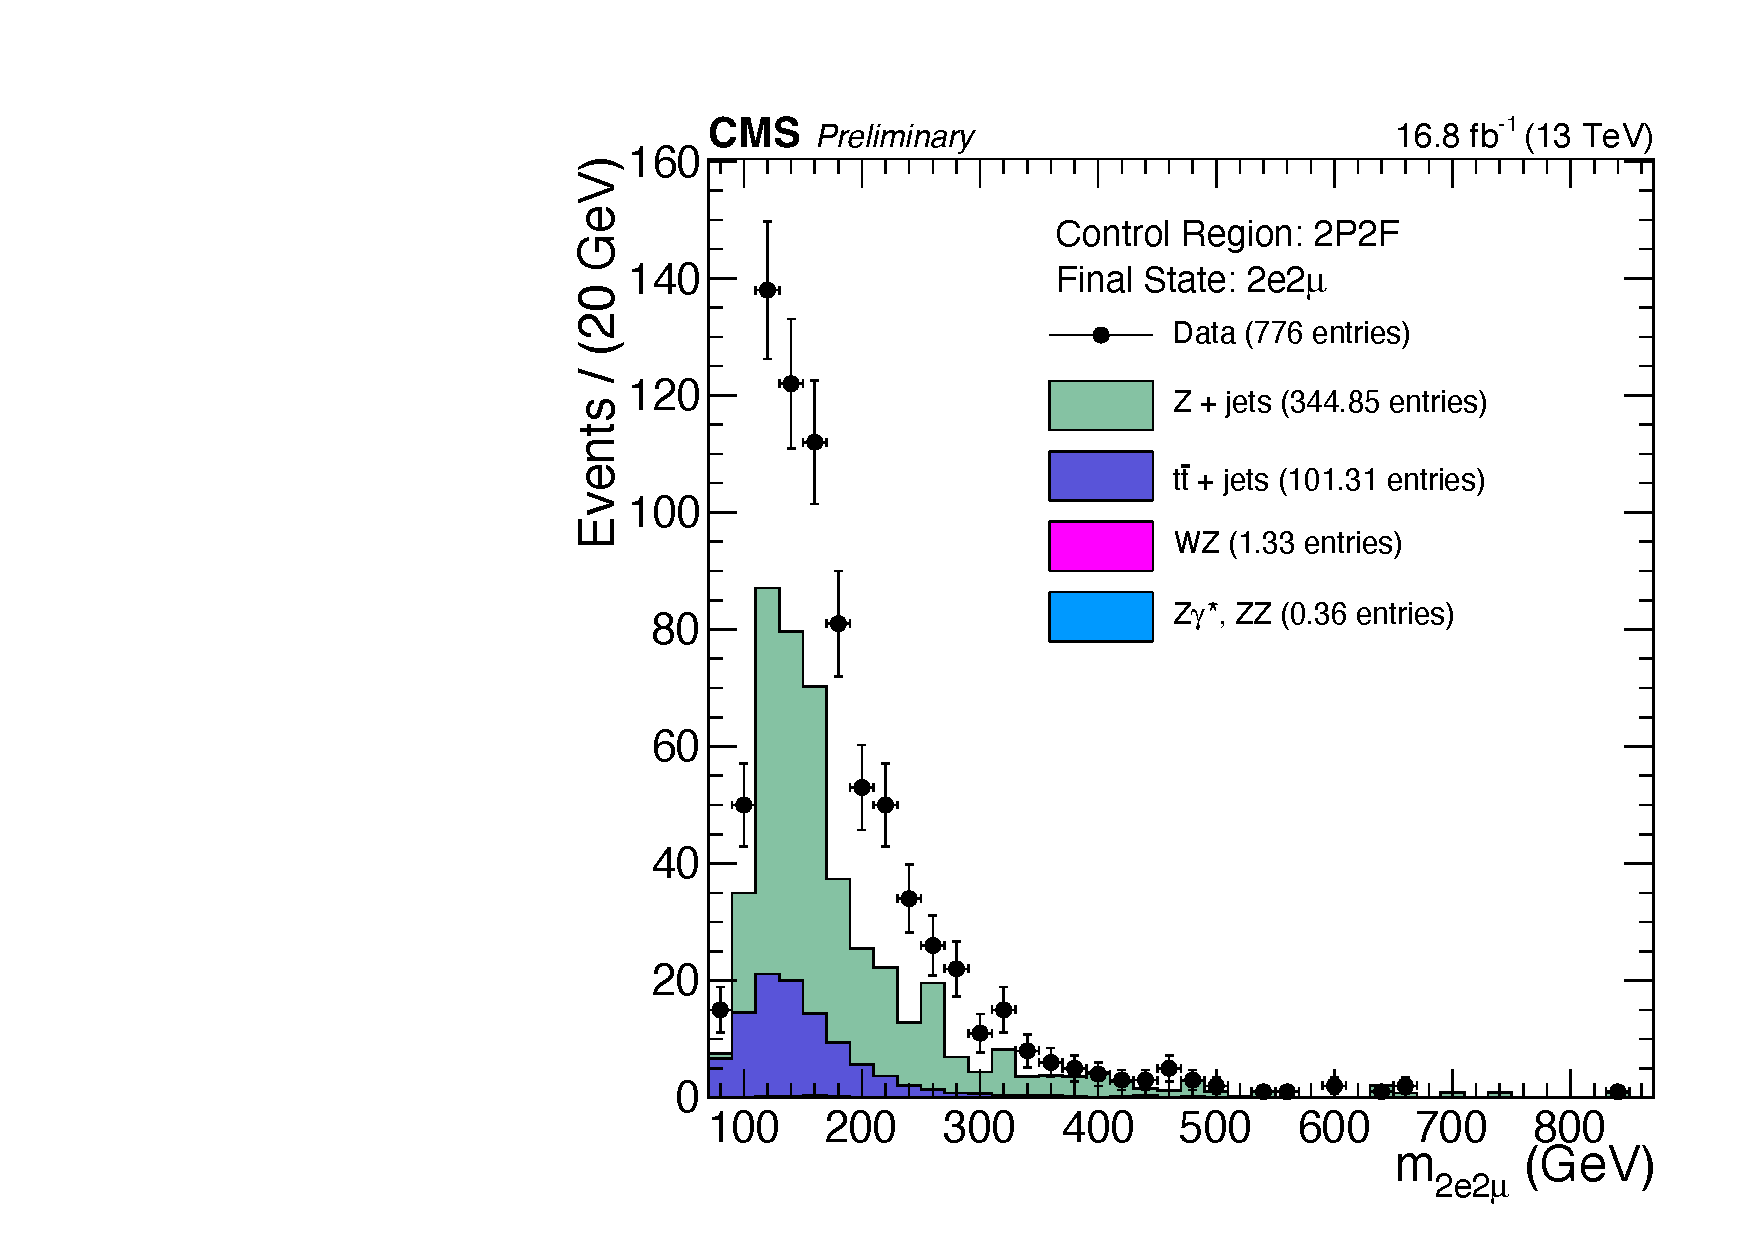
\includegraphics[width=0.48\textwidth]{figures/higgsmassmeas/redbkg/cr/UL2016postVFP_CR_2P2F_2e2mu.pdf}
		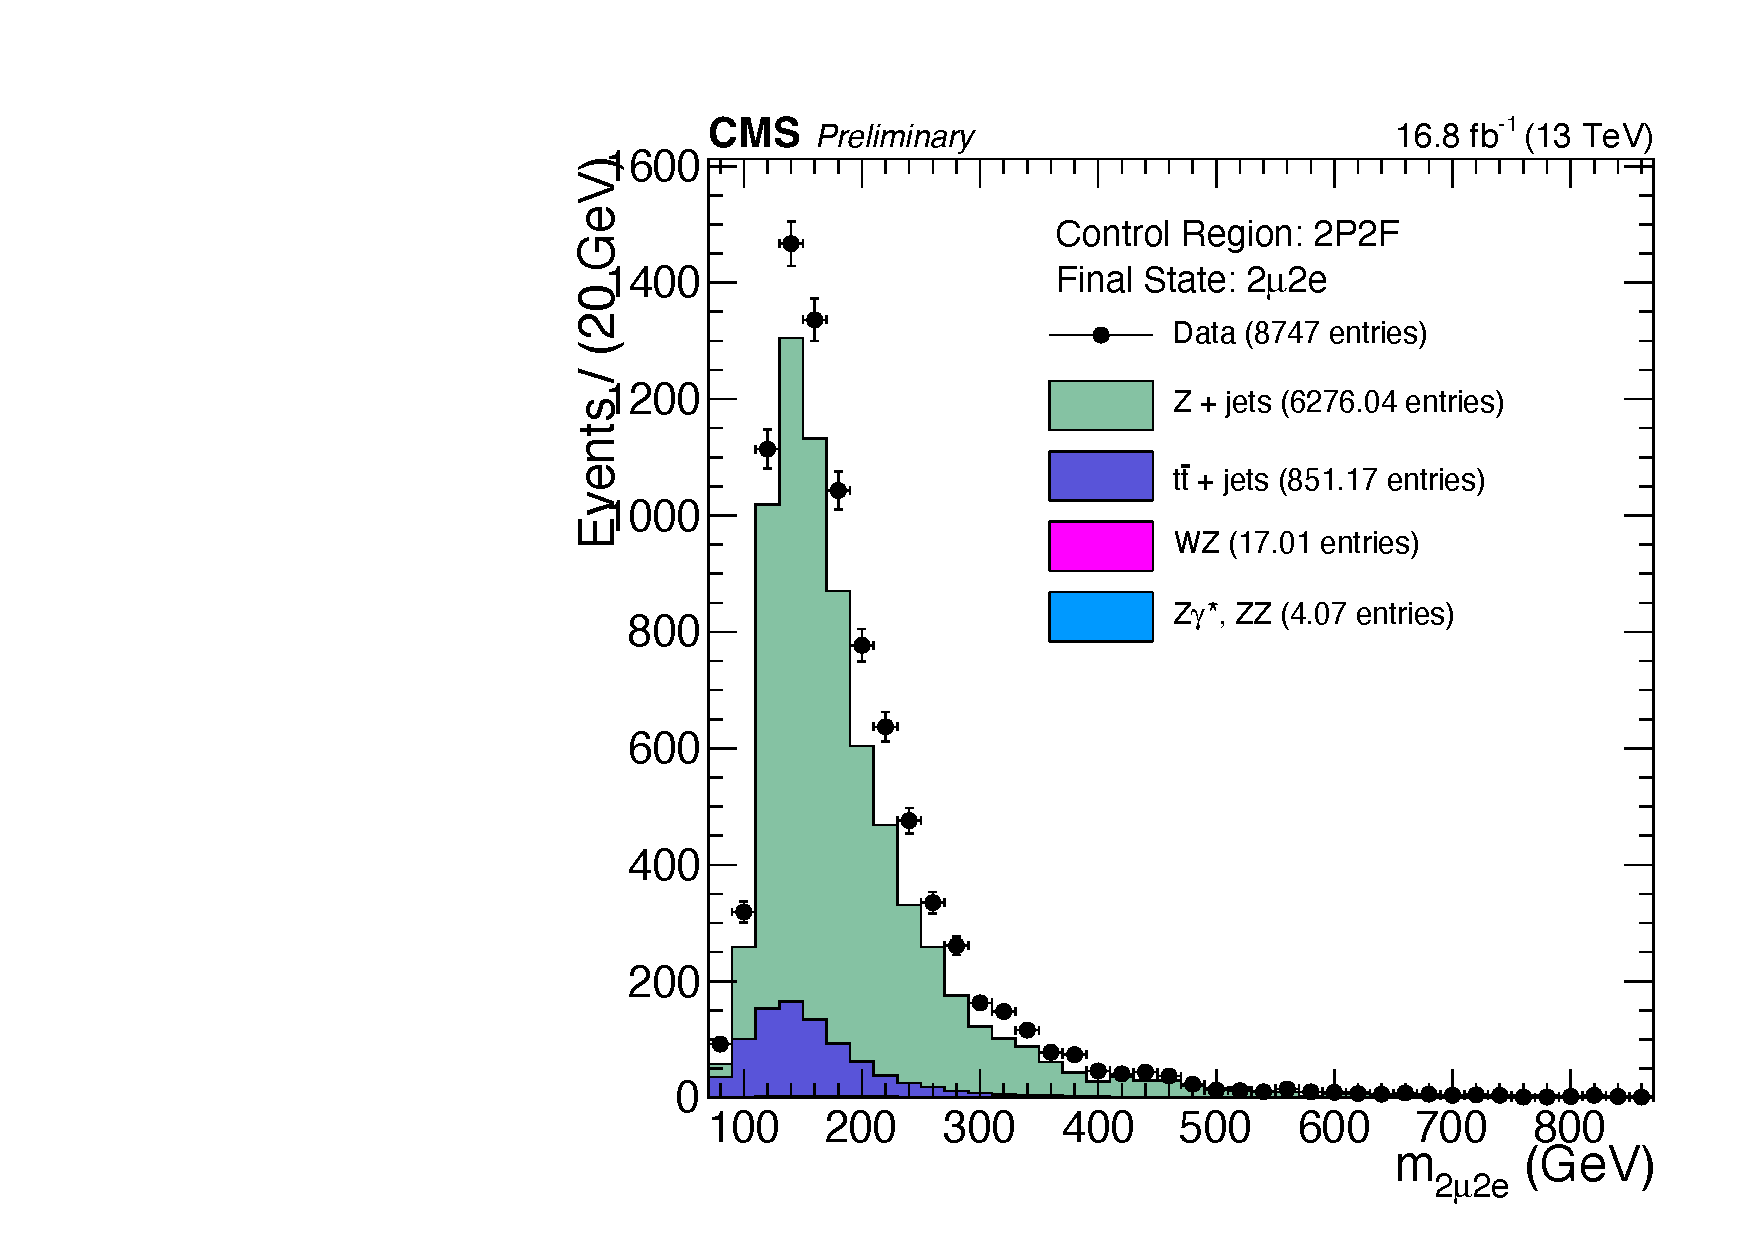
\includegraphics[width=0.48\textwidth]{figures/higgsmassmeas/redbkg/cr/UL2016postVFP_CR_2P2F_2mu2e.pdf}
		\caption{
			Events from 2016 post-VFP UL data that pass 2P2F CR selections (black markers) 
			are compared to the stacked 2P2F distributions of simulated samples
			(\Zplusjets, \ttbarplusjets, \WZ, \ZZ, \Zgammastar).
			The results are split into the $4\ell$ final states:
            $4\mu$ (top left), 4e (top right), 2e2$\mu$ (bottom left), 2$\mu$2e (bottom right).
        }
		\label{cr_plots_2p2f_2016postvfp}
	\end{center}
\end{figure}
\begin{figure}[!htbp]
	\begin{center}
		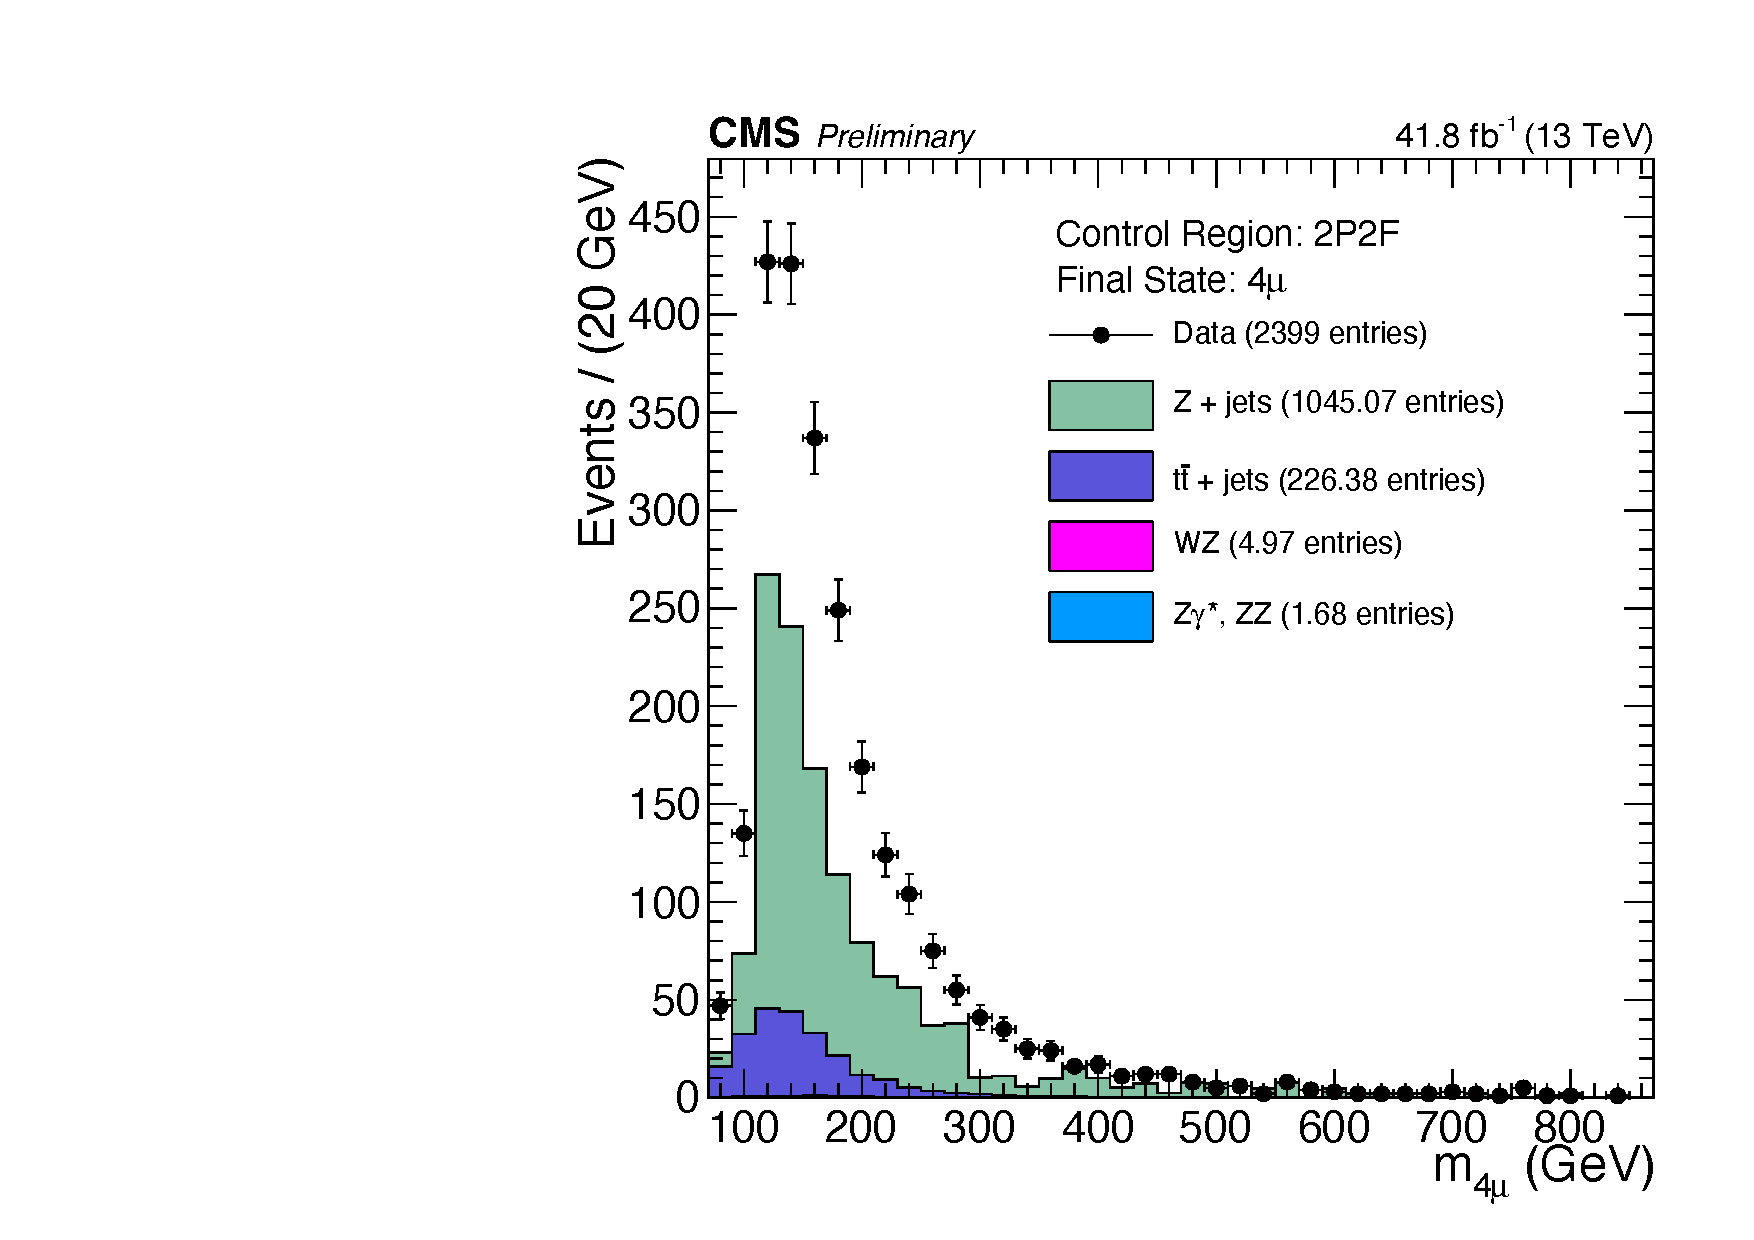
\includegraphics[width=0.48\textwidth]{figures/higgsmassmeas/redbkg/cr/UL2017_CR_2P2F_4mu.pdf}
		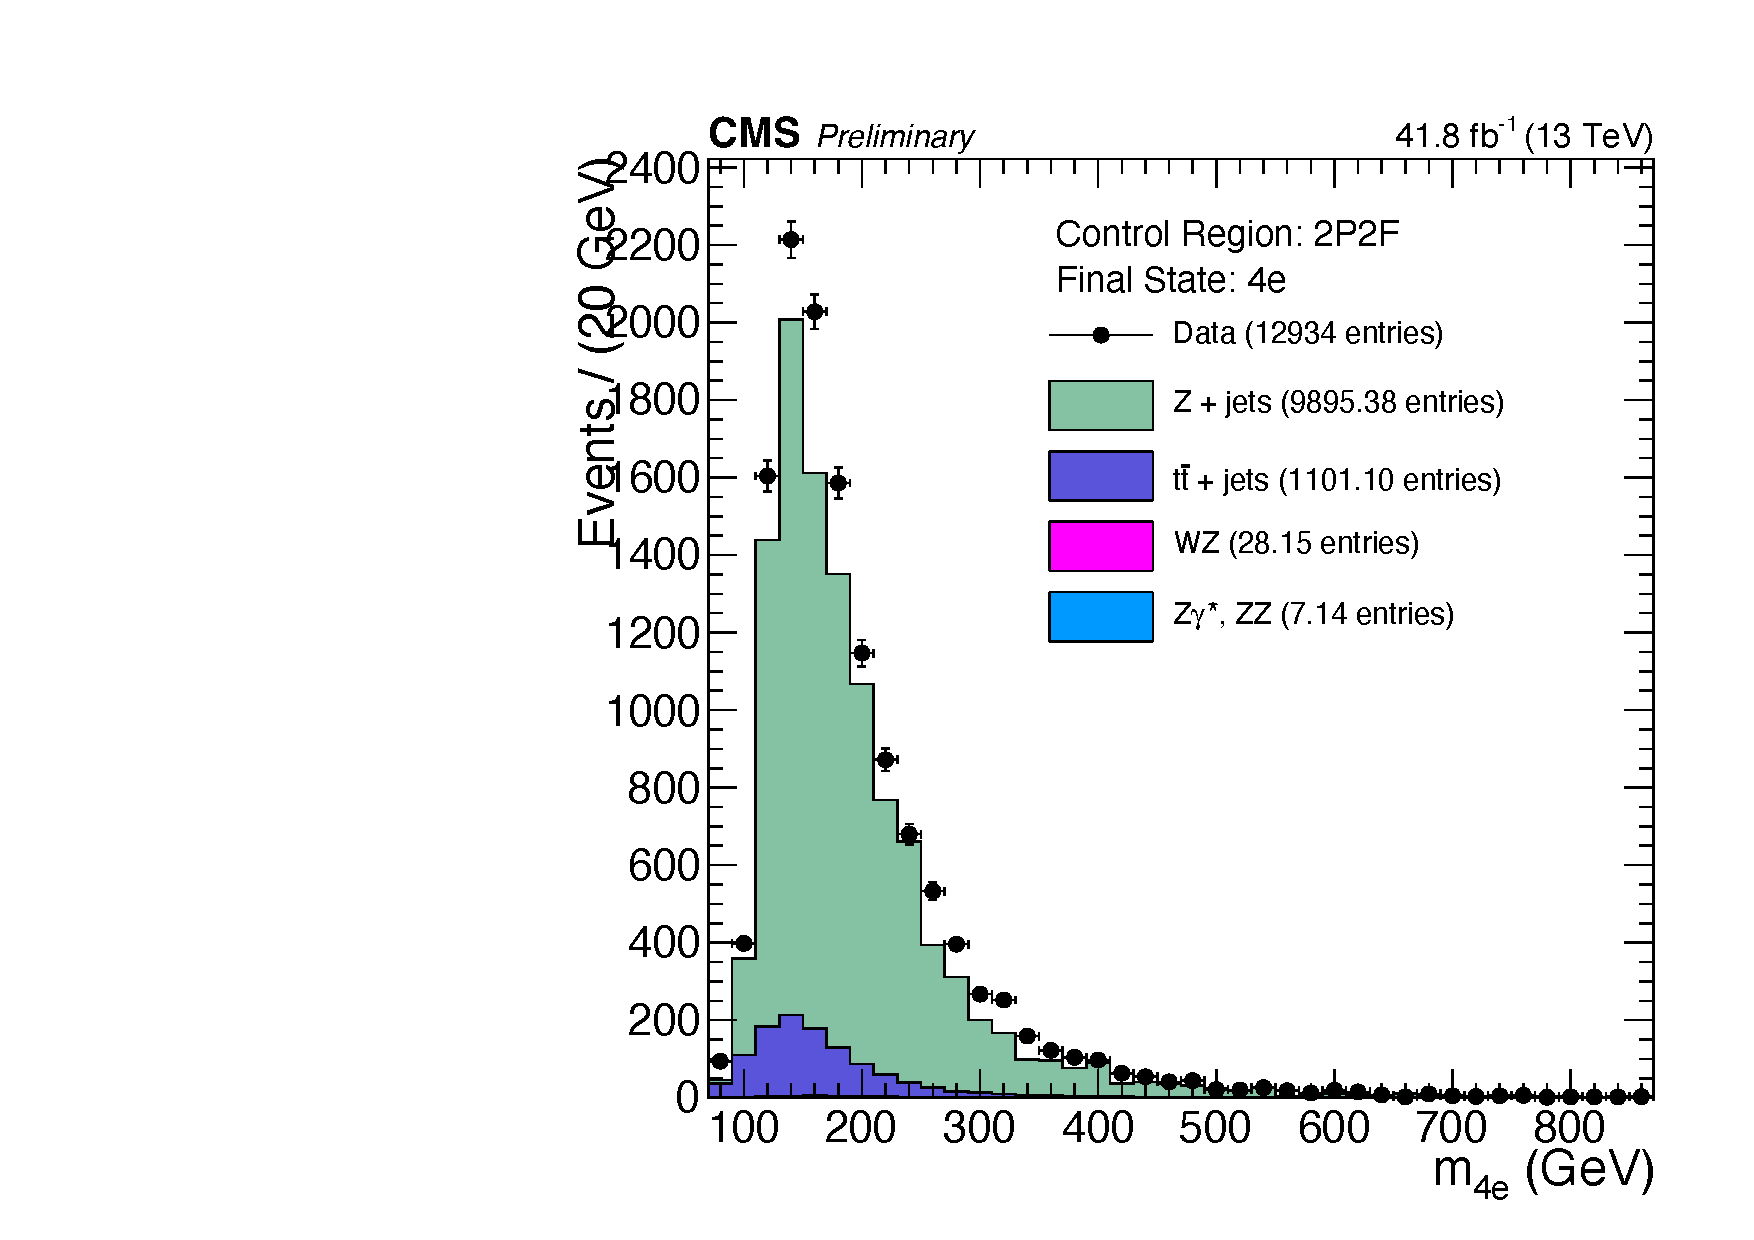
\includegraphics[width=0.48\textwidth]{figures/higgsmassmeas/redbkg/cr/UL2017_CR_2P2F_4e.pdf}
		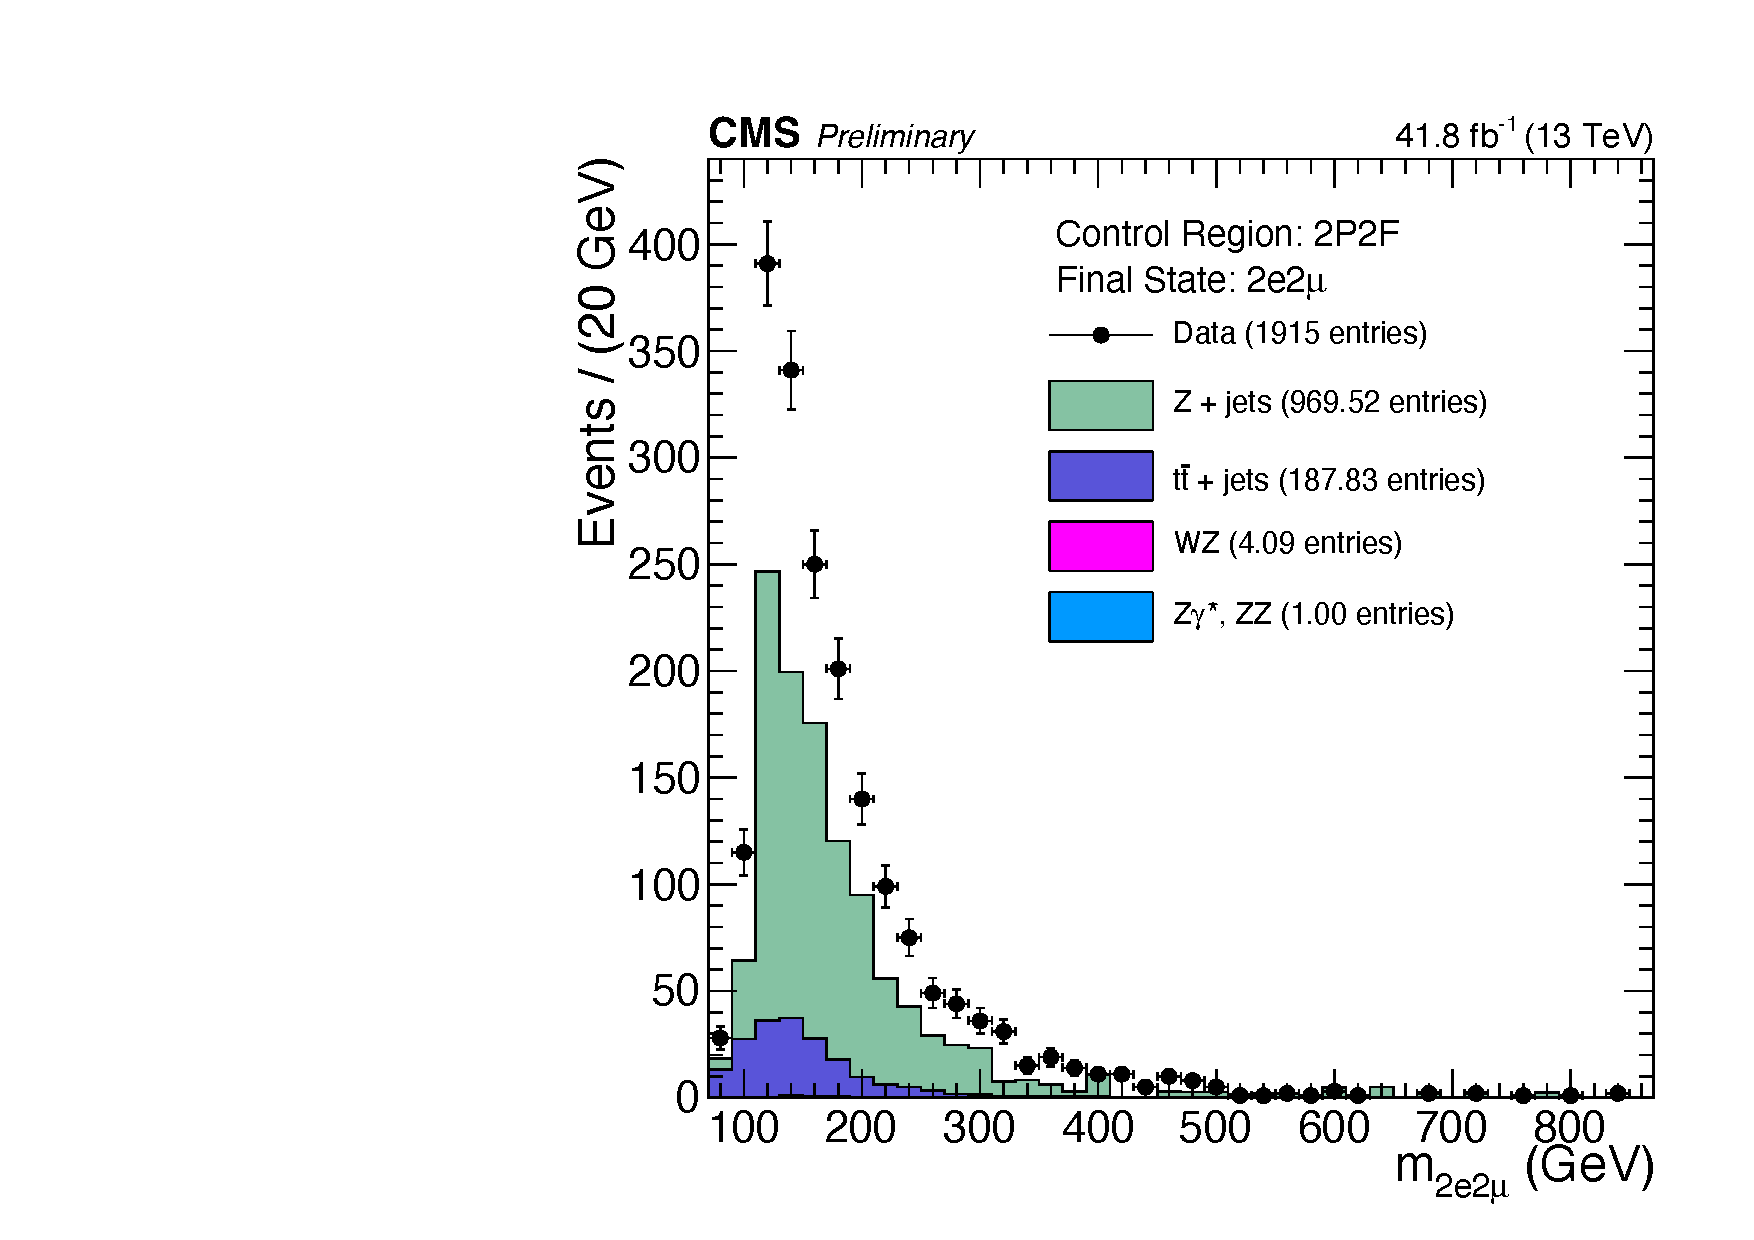
\includegraphics[width=0.48\textwidth]{figures/higgsmassmeas/redbkg/cr/UL2017_CR_2P2F_2e2mu.pdf}
		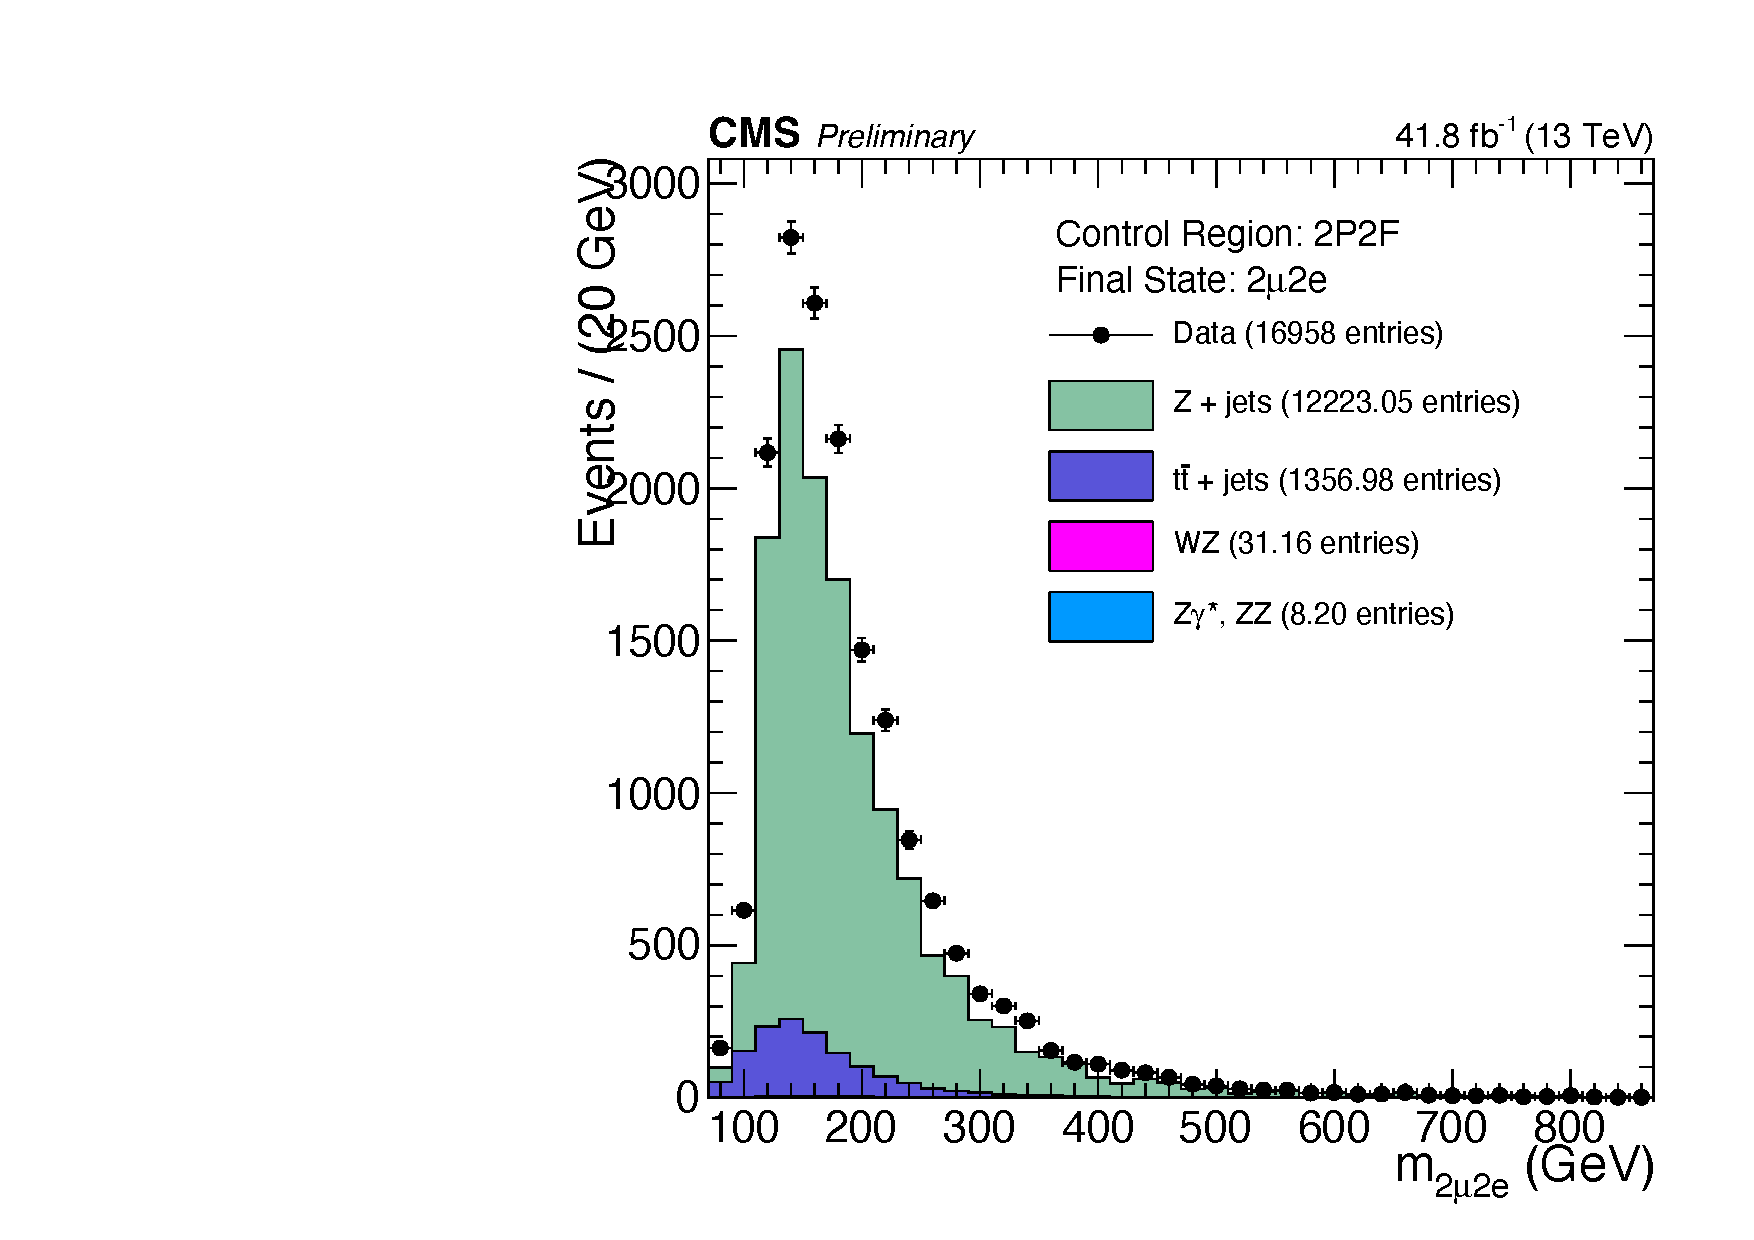
\includegraphics[width=0.48\textwidth]{figures/higgsmassmeas/redbkg/cr/UL2017_CR_2P2F_2mu2e.pdf}
		\caption{
			Events from 2017 UL data that pass 2P2F CR selections (black markers) 
			are compared to the stacked 2P2F distributions of simulated samples
			(\Zplusjets, \ttbarplusjets, \WZ, \ZZ, \Zgammastar).
			The results are split into the $4\ell$ final states:
			$4\mu$ (top left), 4e (top right), 2e2$\mu$ (bottom left), 2$\mu$2e (bottom right).
		}
		\label{cr_plots_2p2f_2017}
	\end{center}
\end{figure}
\begin{figure}[!htbp]
	\begin{center}
		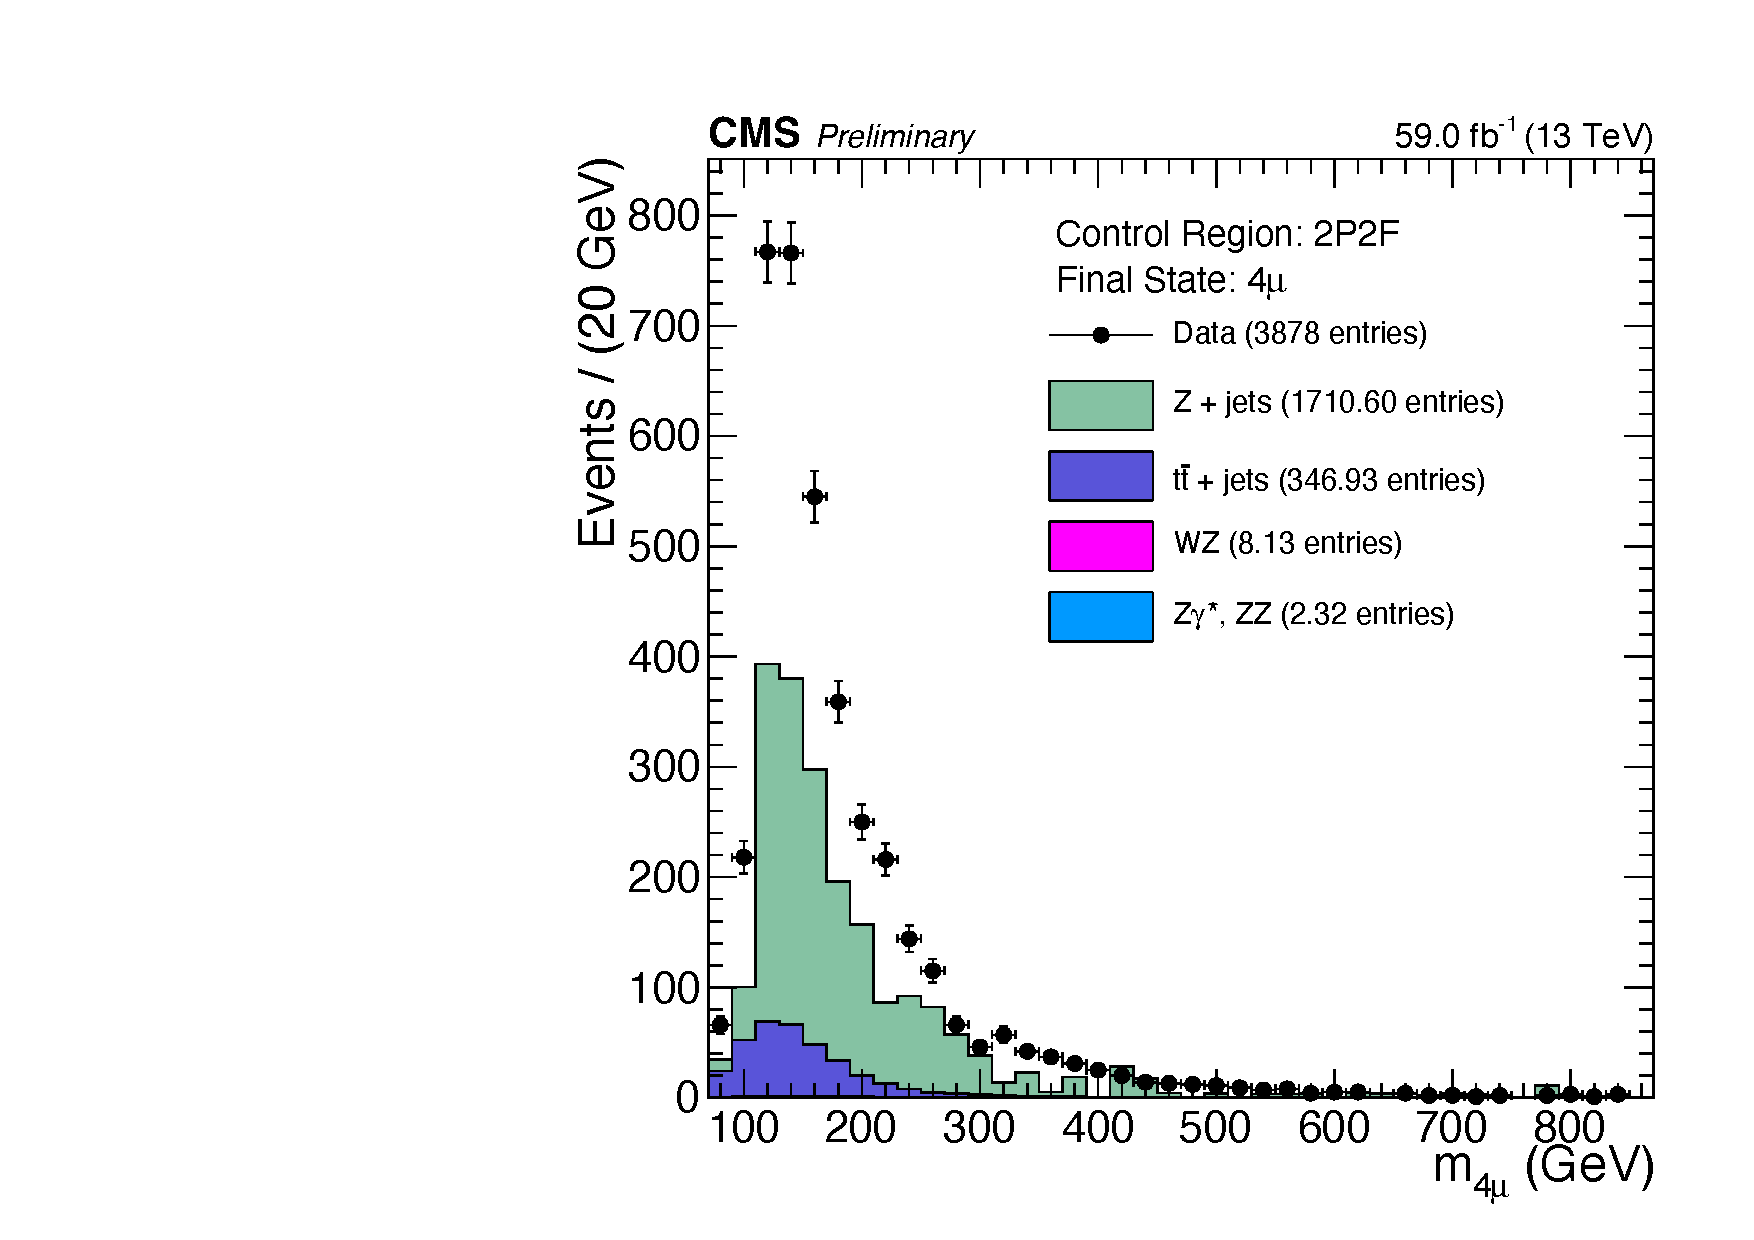
\includegraphics[width=0.48\textwidth]{figures/higgsmassmeas/redbkg/cr/UL2018_CR_2P2F_4mu.pdf}
		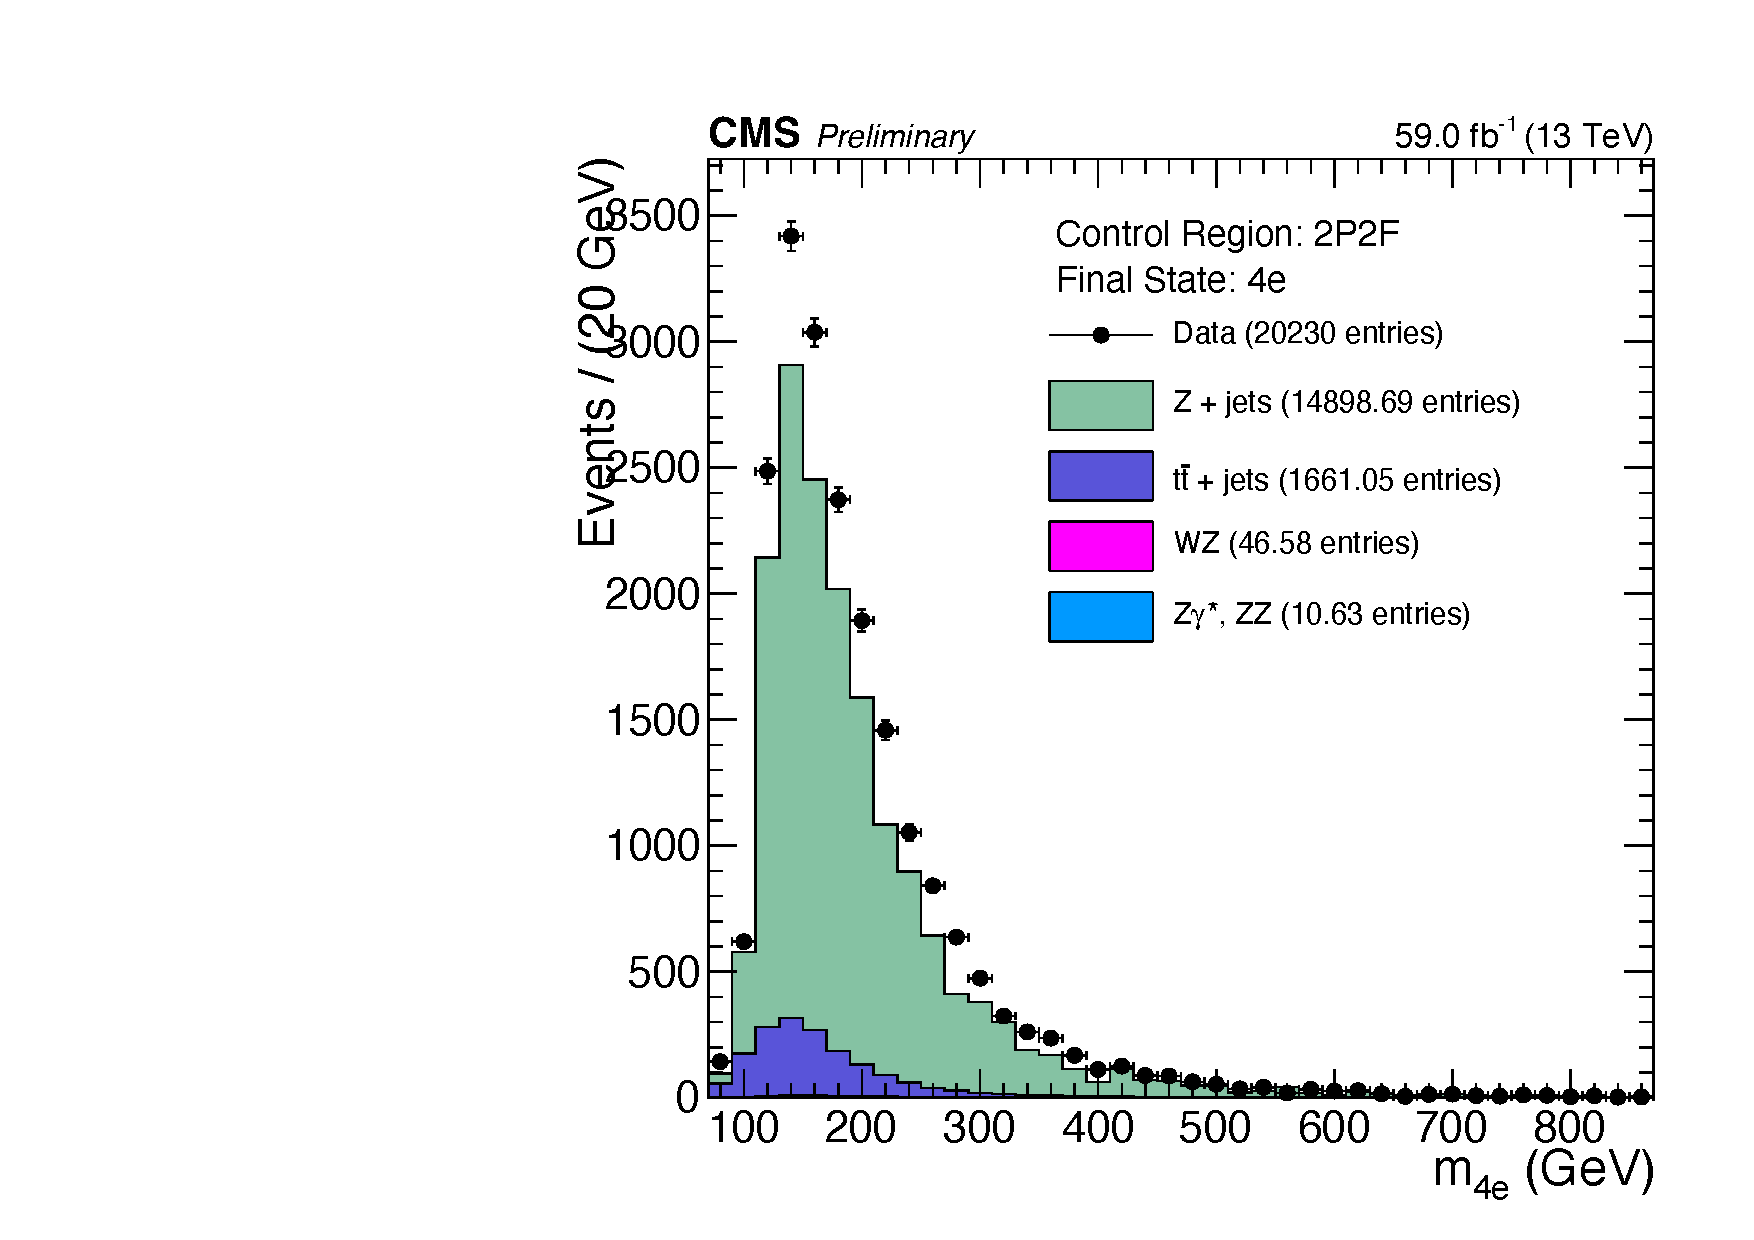
\includegraphics[width=0.48\textwidth]{figures/higgsmassmeas/redbkg/cr/UL2018_CR_2P2F_4e.pdf}
		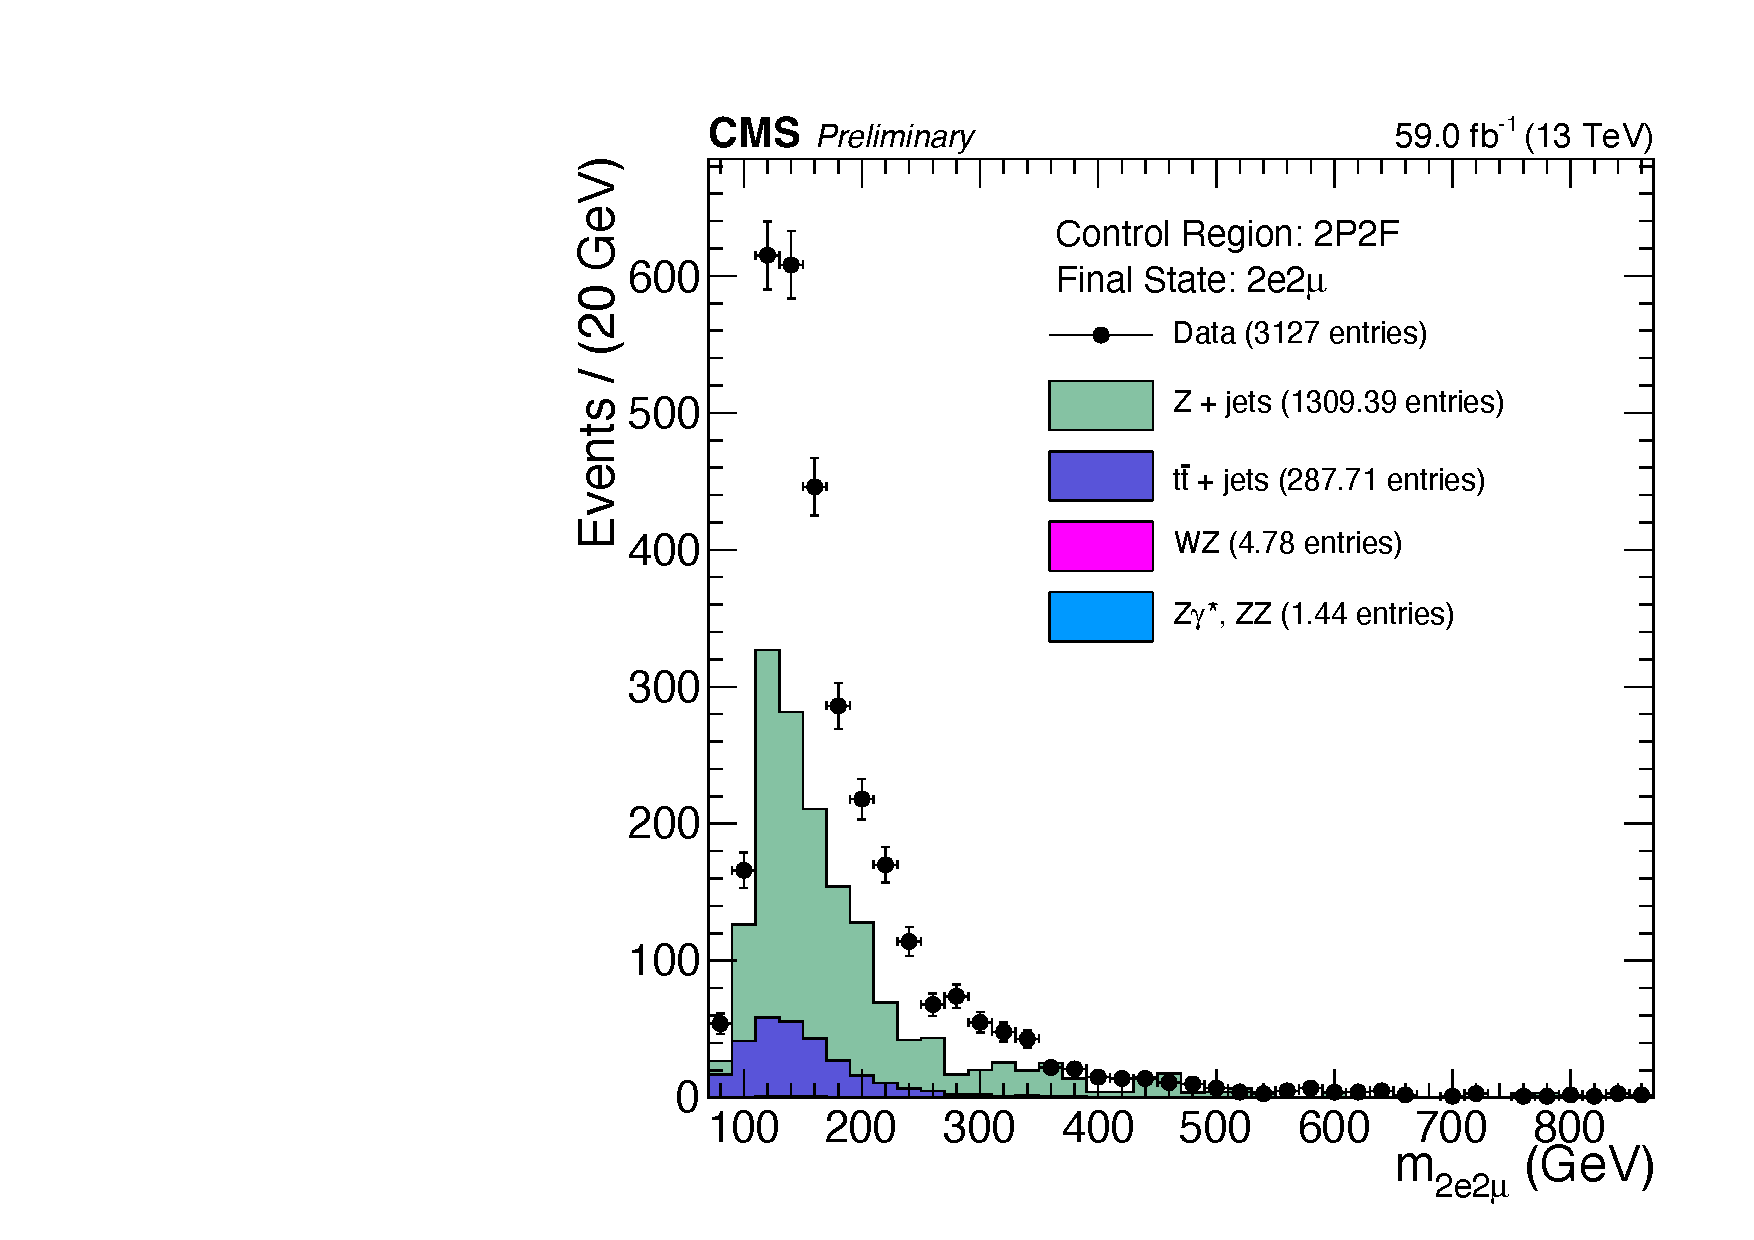
\includegraphics[width=0.48\textwidth]{figures/higgsmassmeas/redbkg/cr/UL2018_CR_2P2F_2e2mu.pdf}
		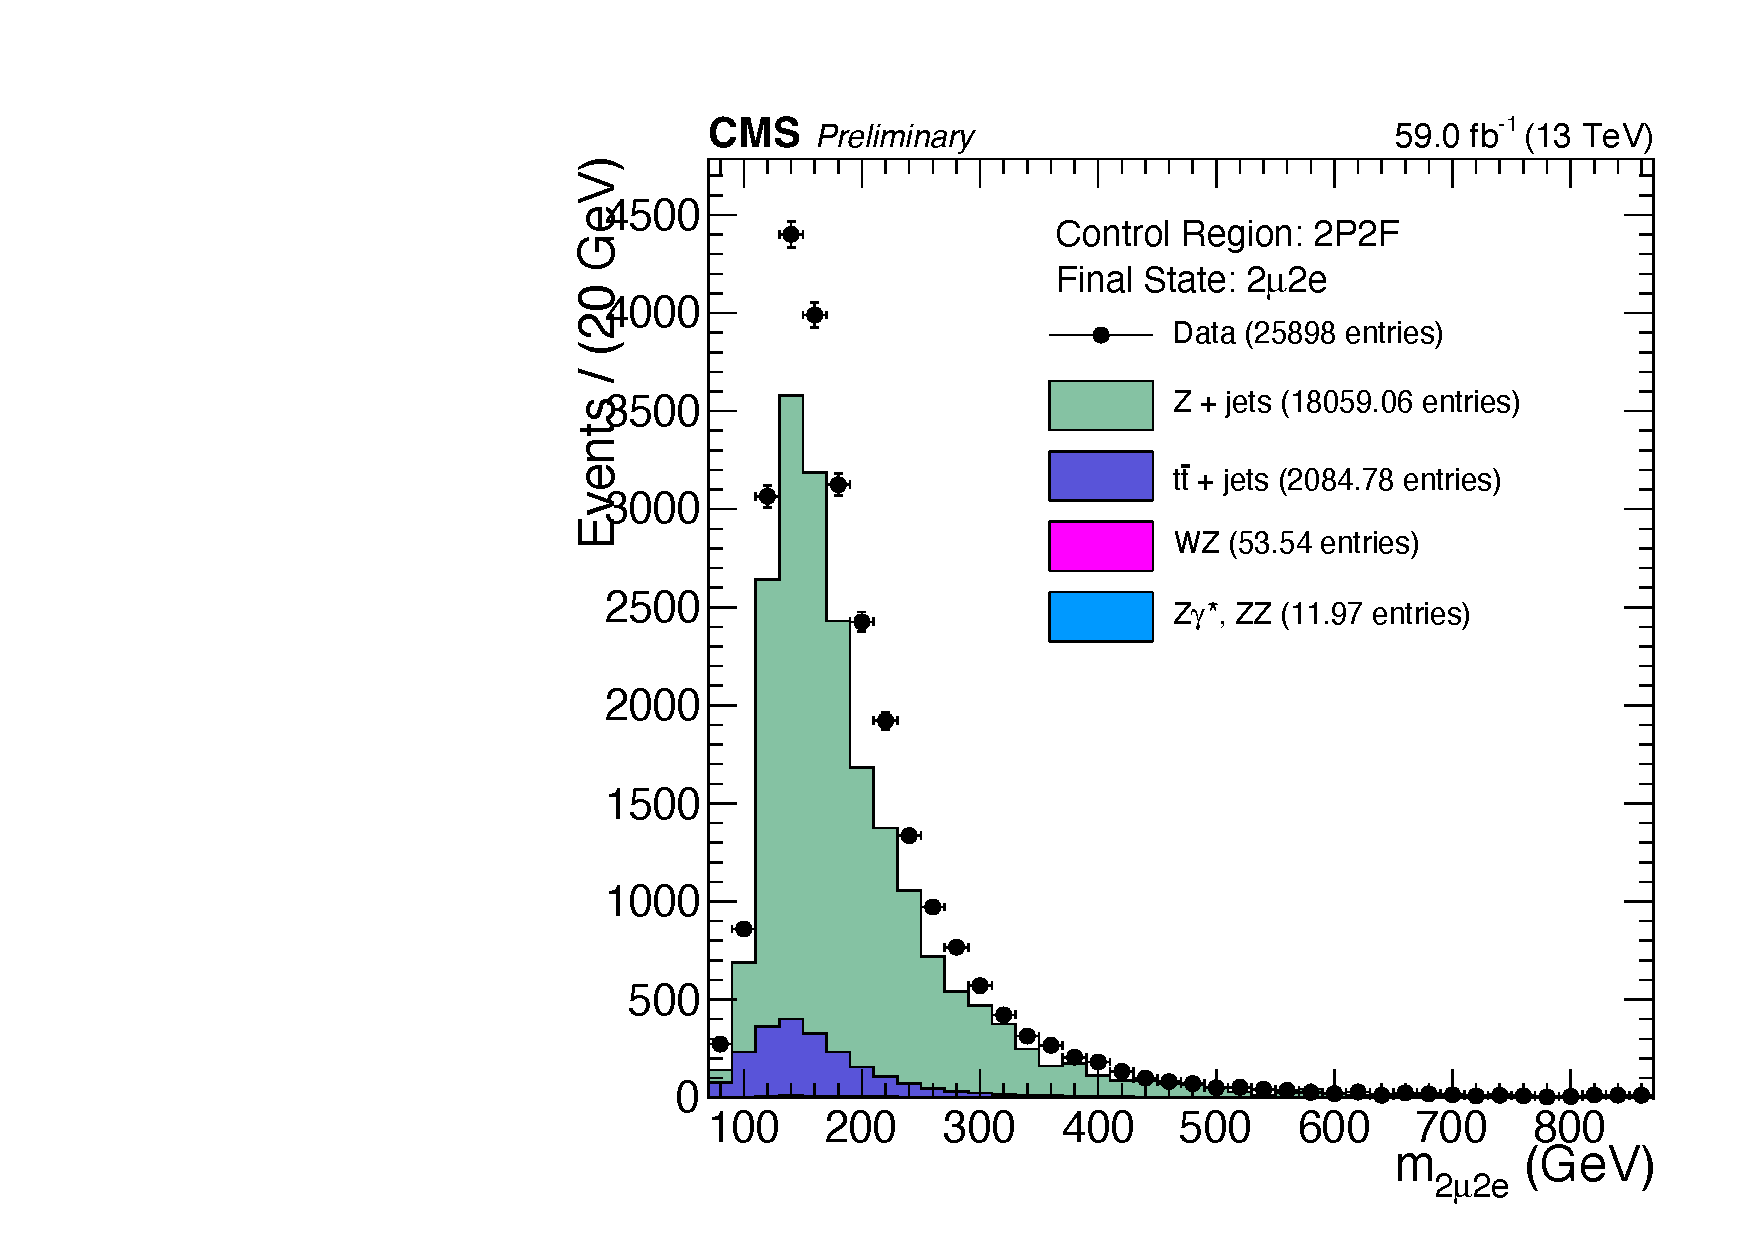
\includegraphics[width=0.48\textwidth]{figures/higgsmassmeas/redbkg/cr/UL2018_CR_2P2F_2mu2e.pdf}
		\caption{
			Events from 2018 UL data that pass 2P2F CR selections (black markers) 
			are compared to the stacked 2P2F distributions of simulated samples
			(\Zplusjets, \ttbarplusjets, \WZ, \ZZ, \Zgammastar).
			The results are split into the $4\ell$ final states:
			$4\mu$ (top left), 4e (top right), 2e2$\mu$ (bottom left), 2$\mu$2e (bottom right).
		}
		\label{cr_plots_2p2f_2018}
	\end{center}
\end{figure}
\begin{figure}[!htbp]
	\begin{center}
		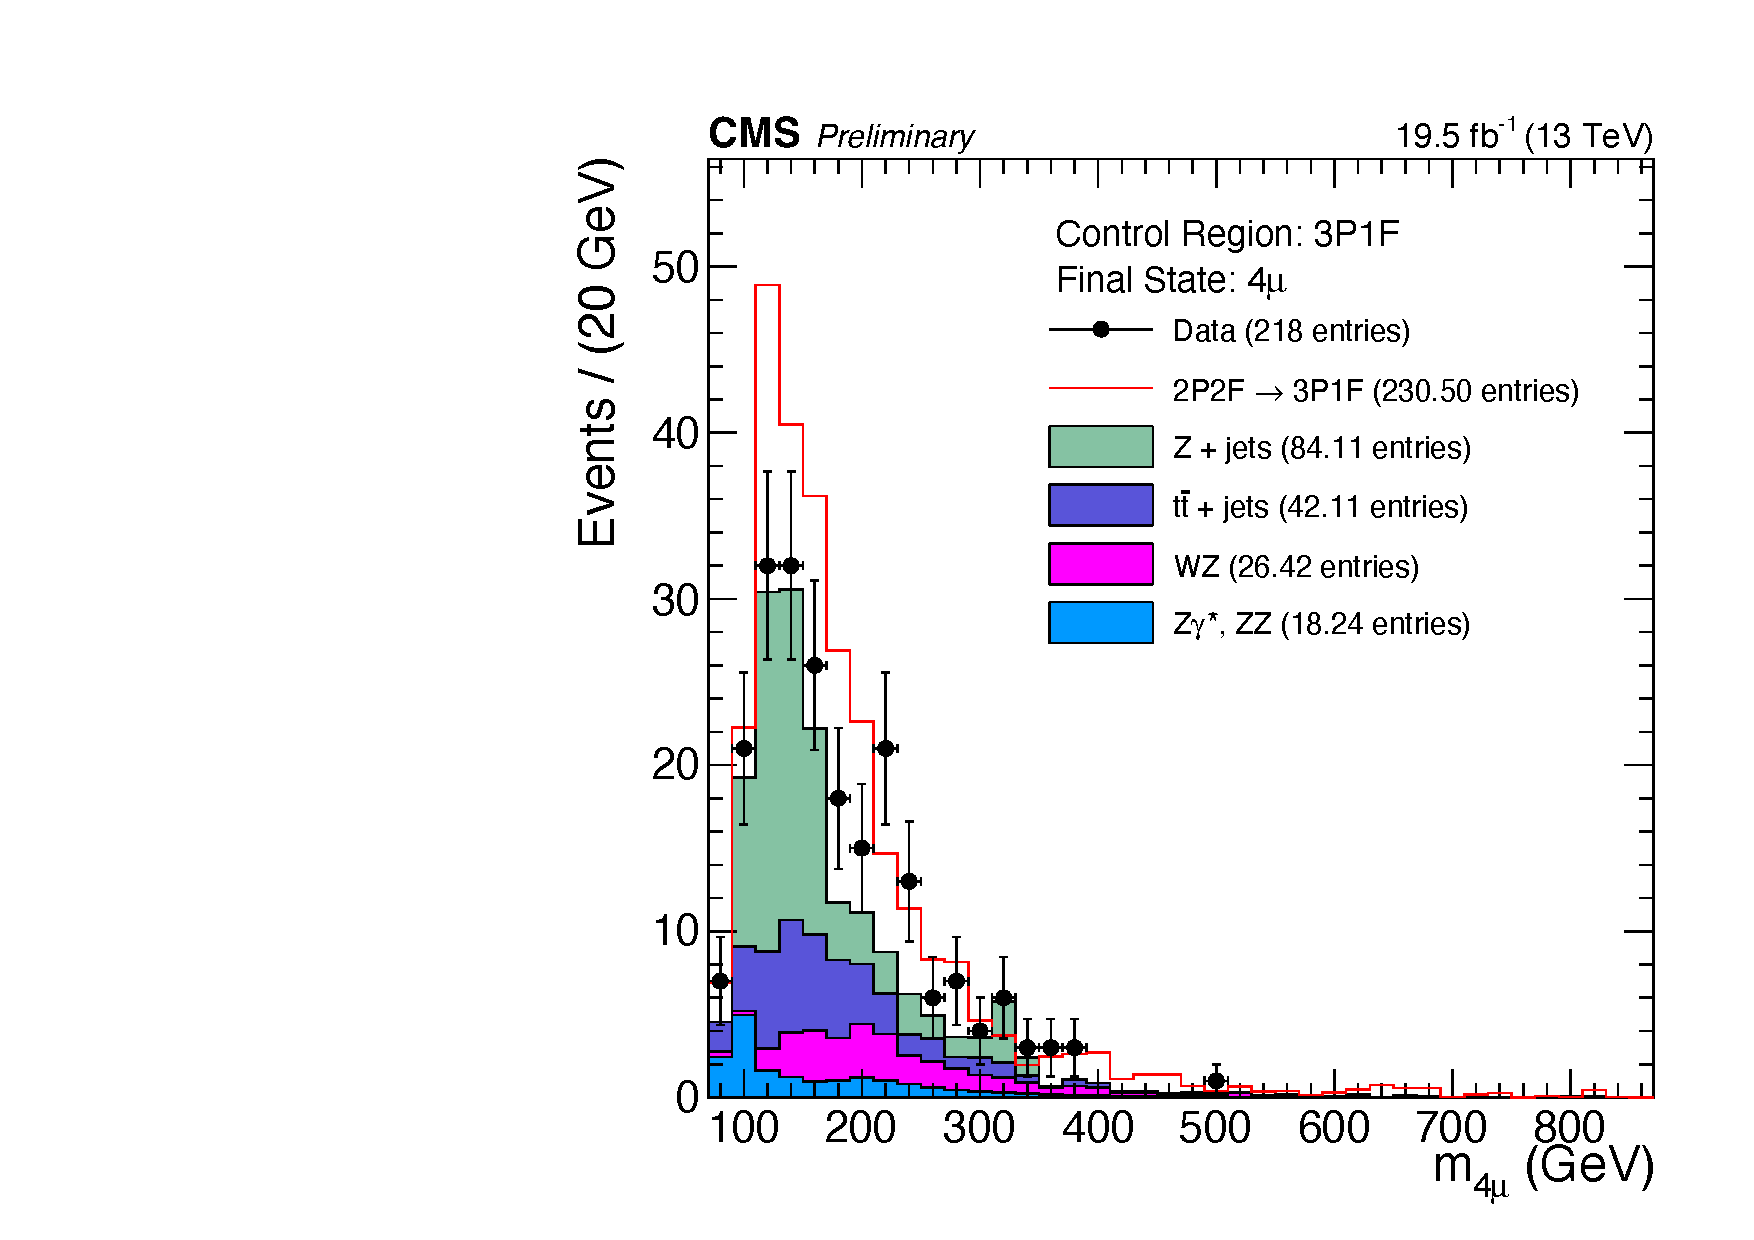
\includegraphics[width=0.48\textwidth]{figures/higgsmassmeas/redbkg/cr/UL2016preVFP_CR_3P1F_4mu.pdf}
		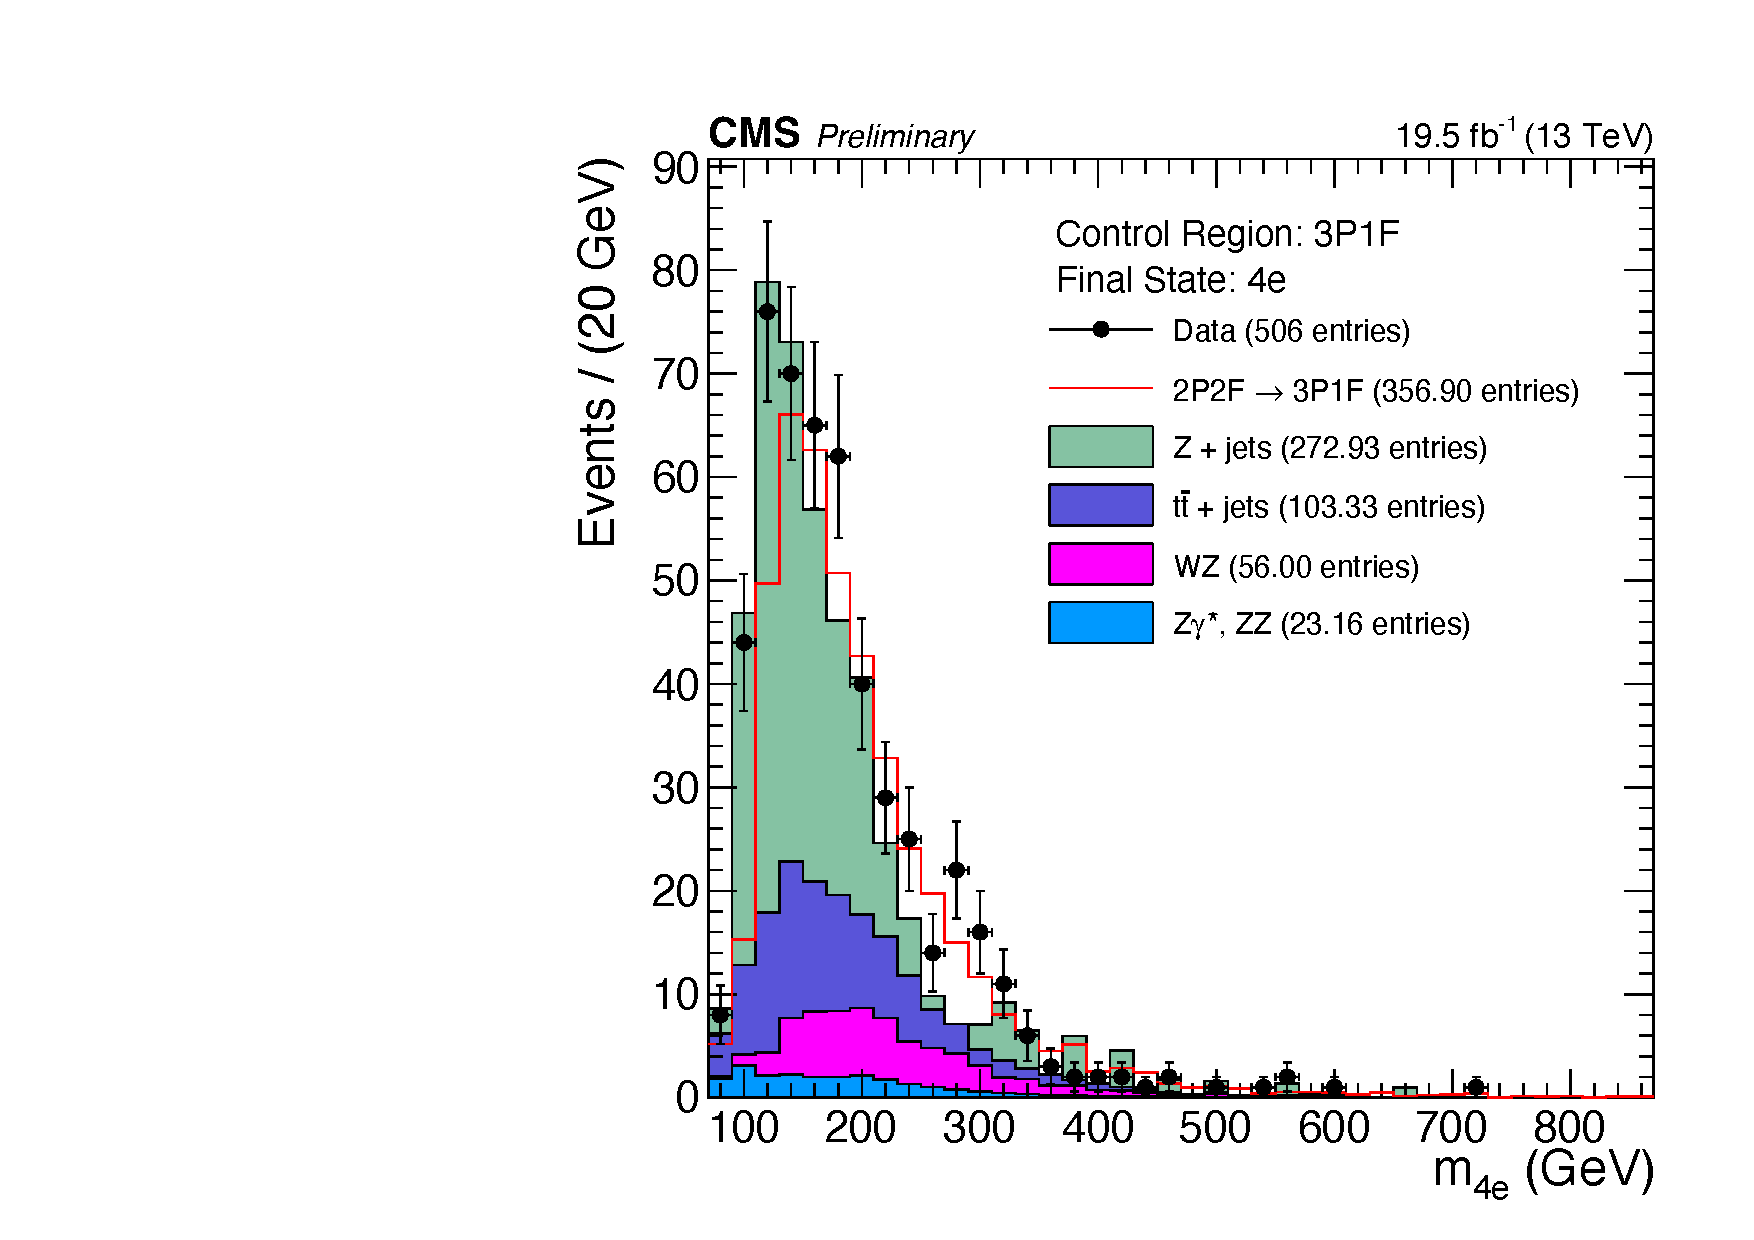
\includegraphics[width=0.48\textwidth]{figures/higgsmassmeas/redbkg/cr/UL2016preVFP_CR_3P1F_4e.pdf}
		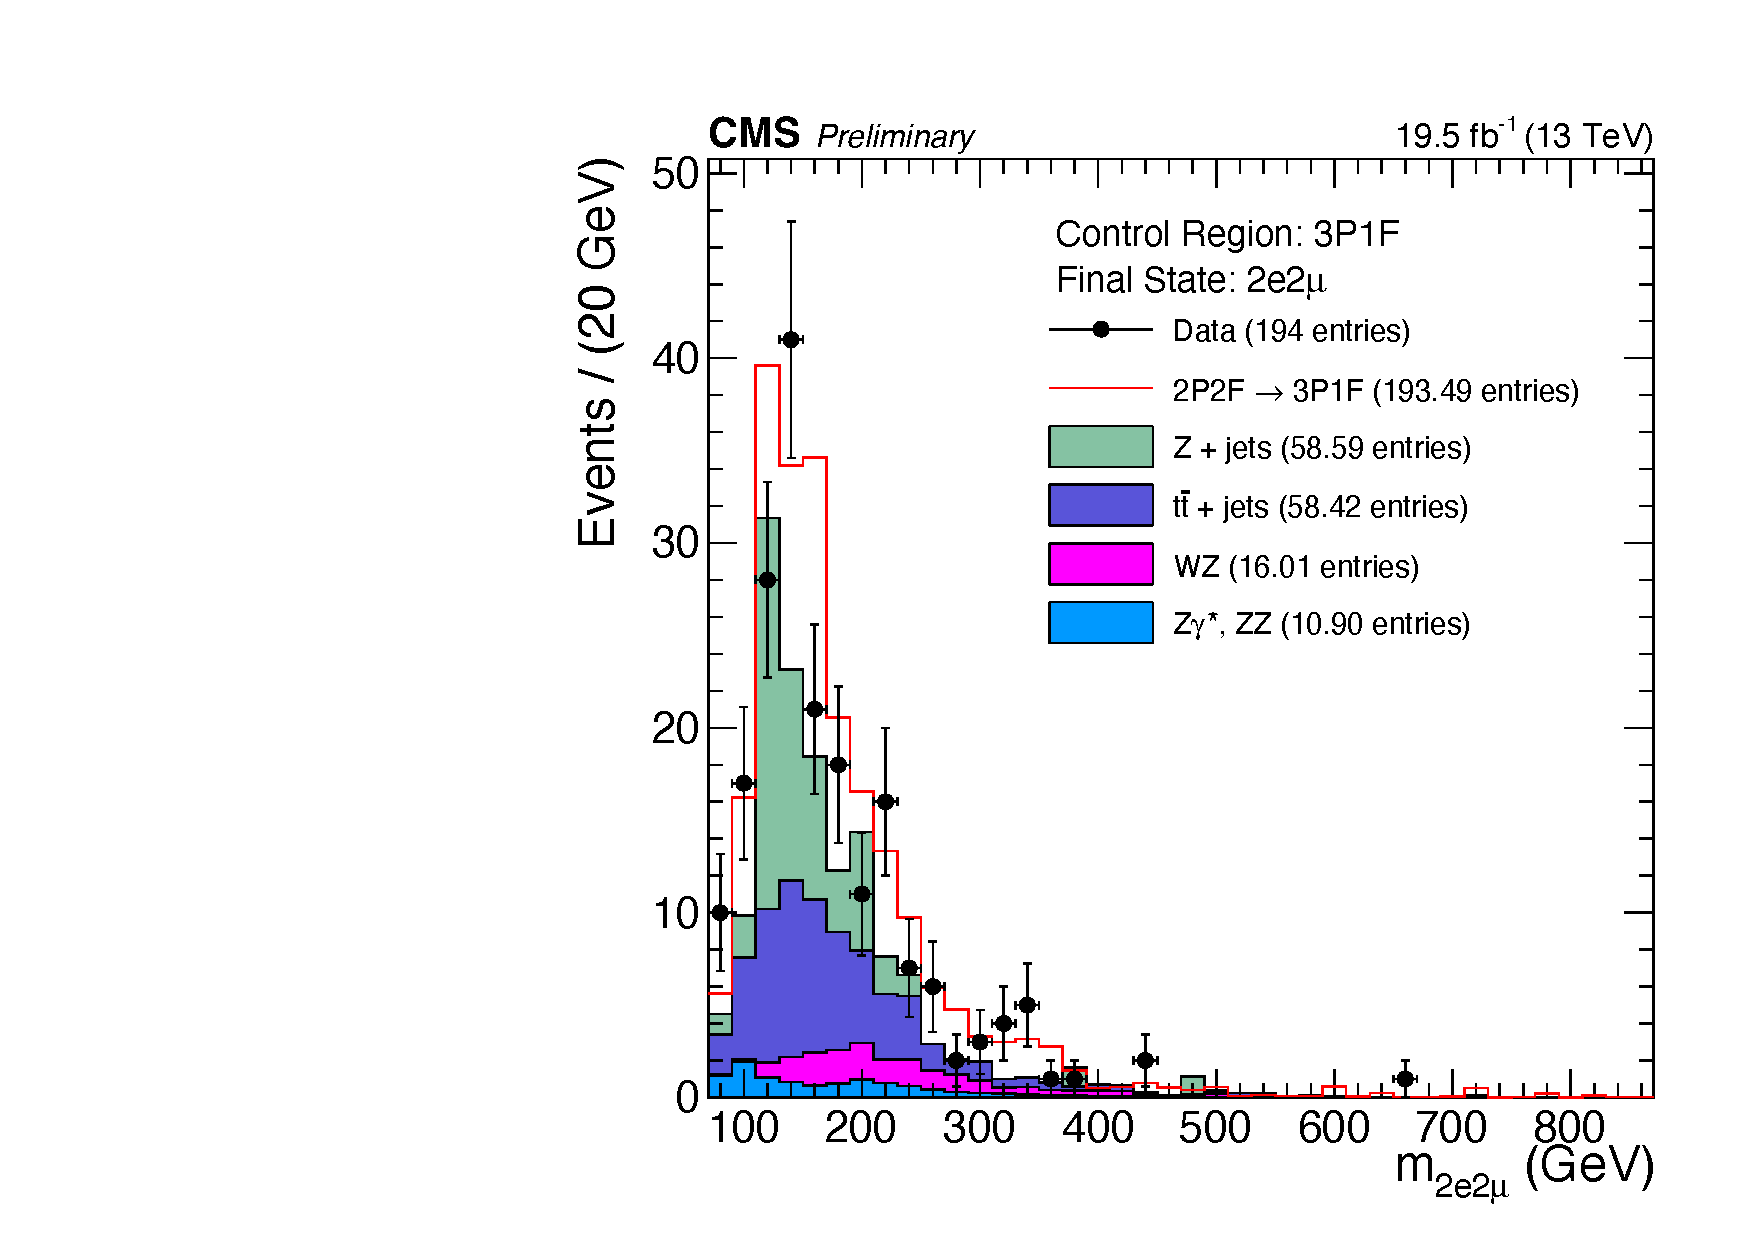
\includegraphics[width=0.48\textwidth]{figures/higgsmassmeas/redbkg/cr/UL2016preVFP_CR_3P1F_2e2mu.pdf}
		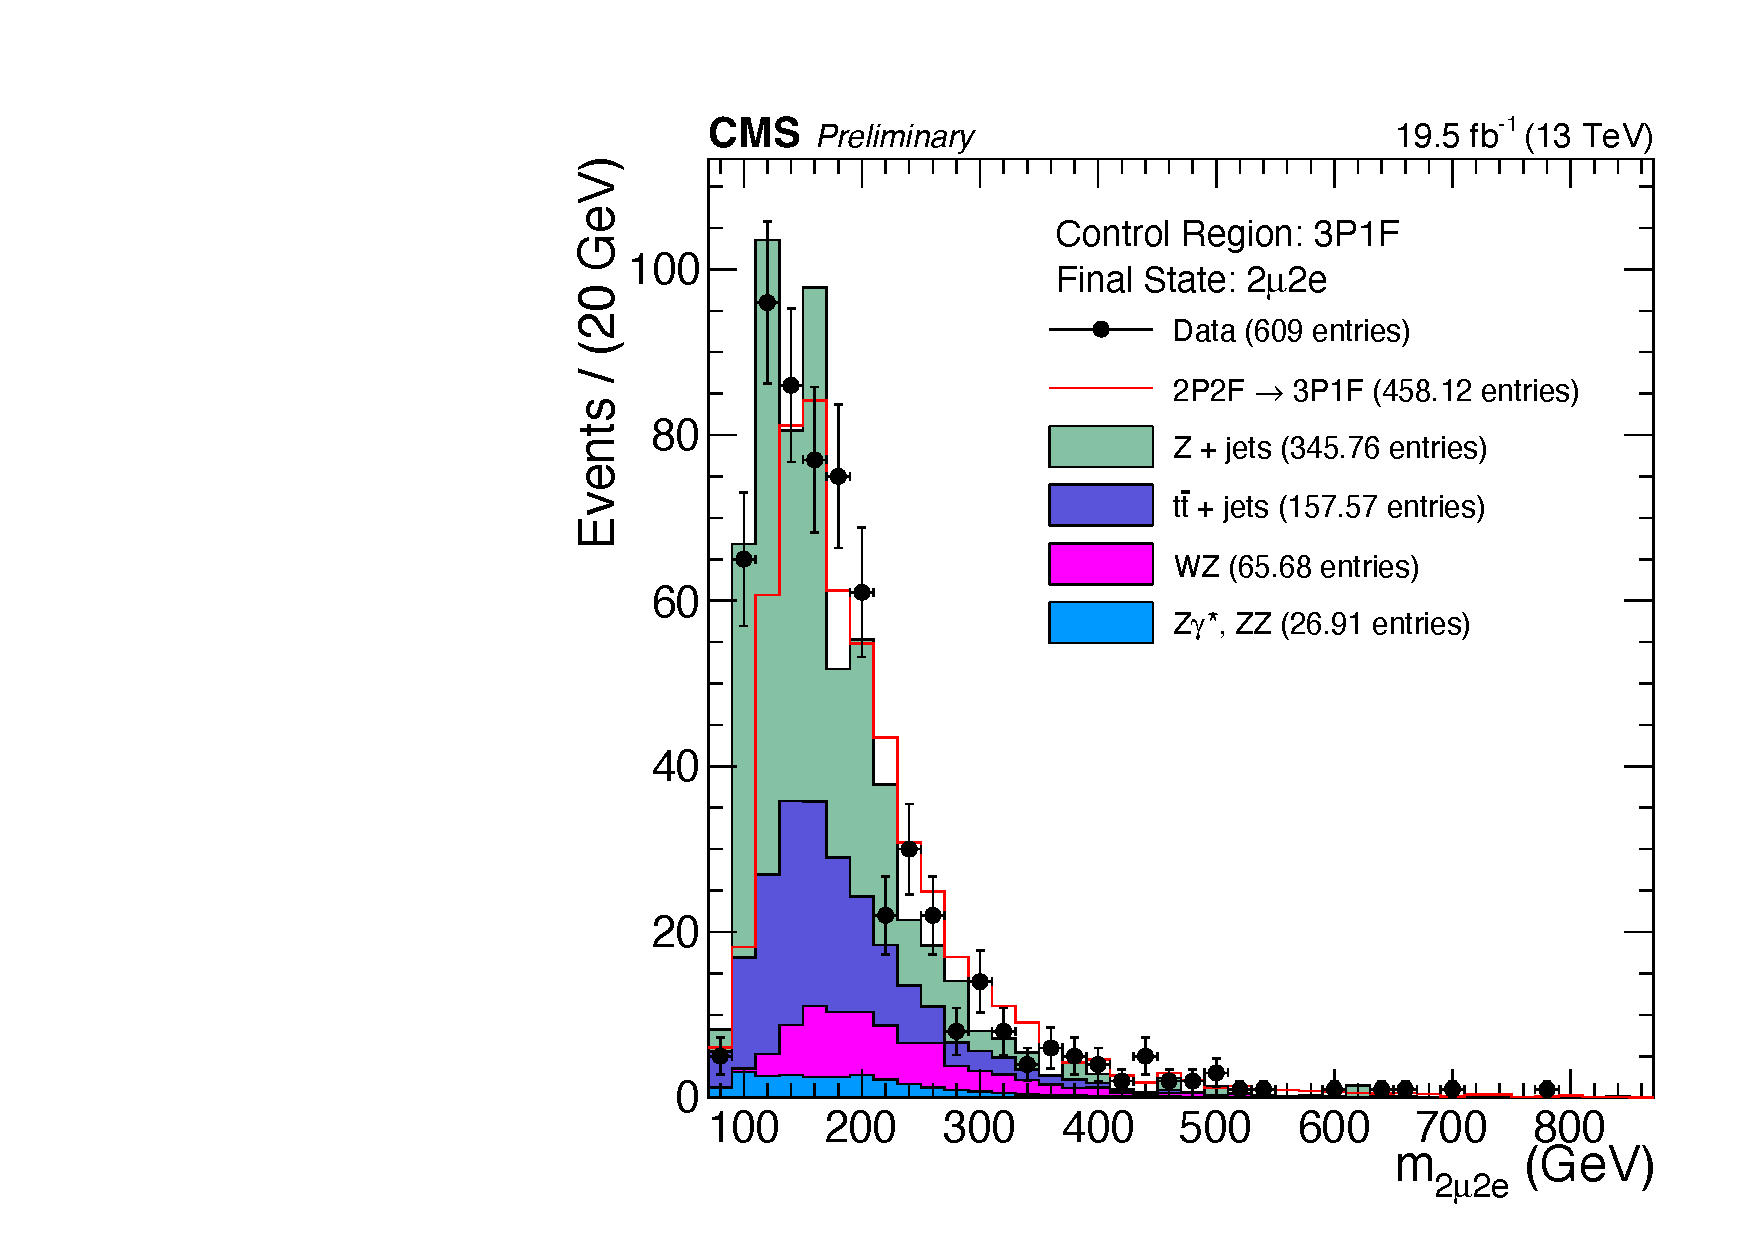
\includegraphics[width=0.48\textwidth]{figures/higgsmassmeas/redbkg/cr/UL2016preVFP_CR_3P1F_2mu2e.pdf}
		\caption{
			Events from 2016 pre-VFP UL data that pass 3P1F CR selections (black markers) 
			are compared to the stacked 3P1F distributions of simulated samples
			(\Zplusjets, \ttbarplusjets, \WZ, \ZZ, \Zgammastar)
			and to the predicted contribution of 2-prompt-2-nonprompt-lepton processes to the 3P1F CR (red line).
			This prediction is obtained by making a distribution of all event weights given by Eq.~\ref{eqn:wt_2prto3p1f_simp} and stacking that on top of the WZ and \ZZ distributions.
			The results are split into the $4\ell$ final states:
			$4\mu$ (top left), 4e (top right), 2e2$\mu$ (bottom left), 2$\mu$2e (bottom right).
		}
		\label{cr_plots_3p1f_2016prevfp}
	\end{center}
\end{figure}
\begin{figure}[!htbp]
	\begin{center}
		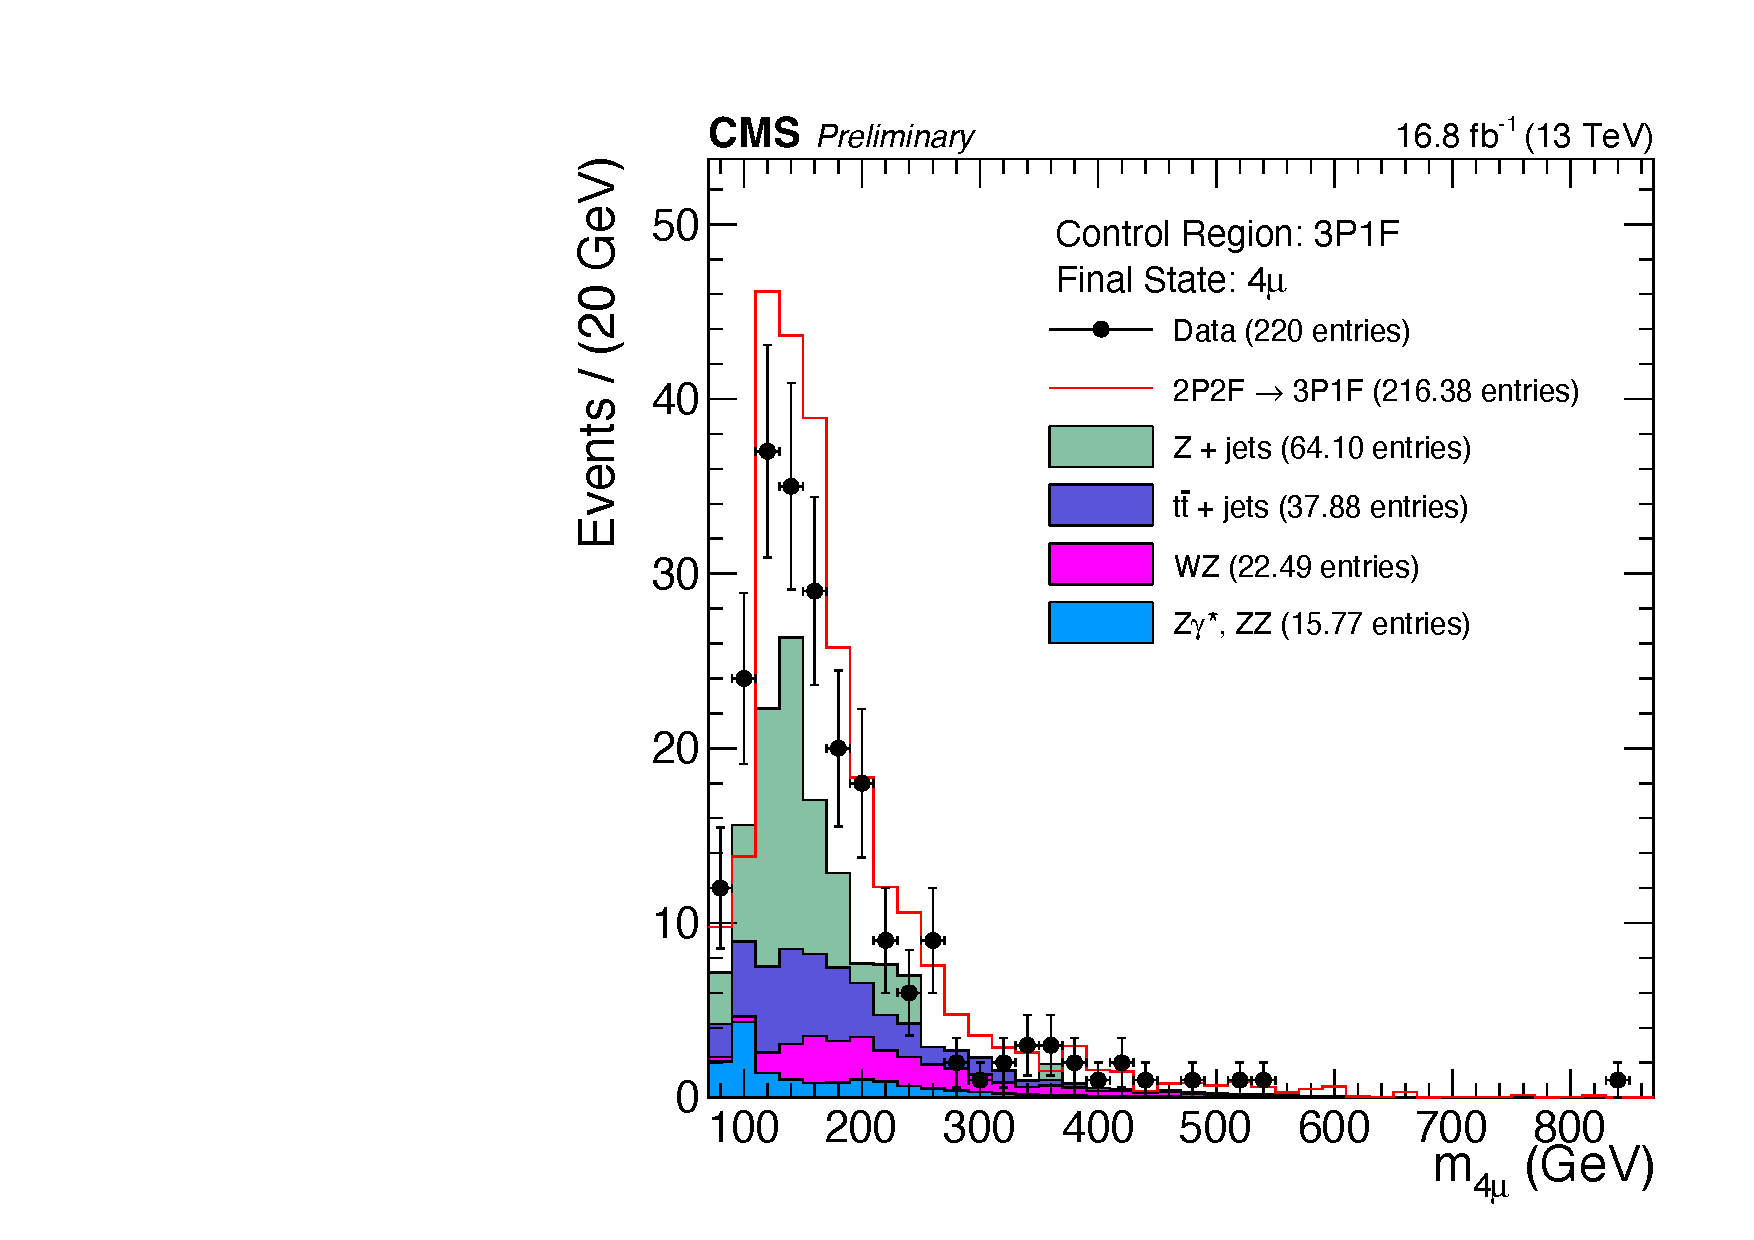
\includegraphics[width=0.48\textwidth]{figures/higgsmassmeas/redbkg/cr/UL2016postVFP_CR_3P1F_4mu.pdf}
		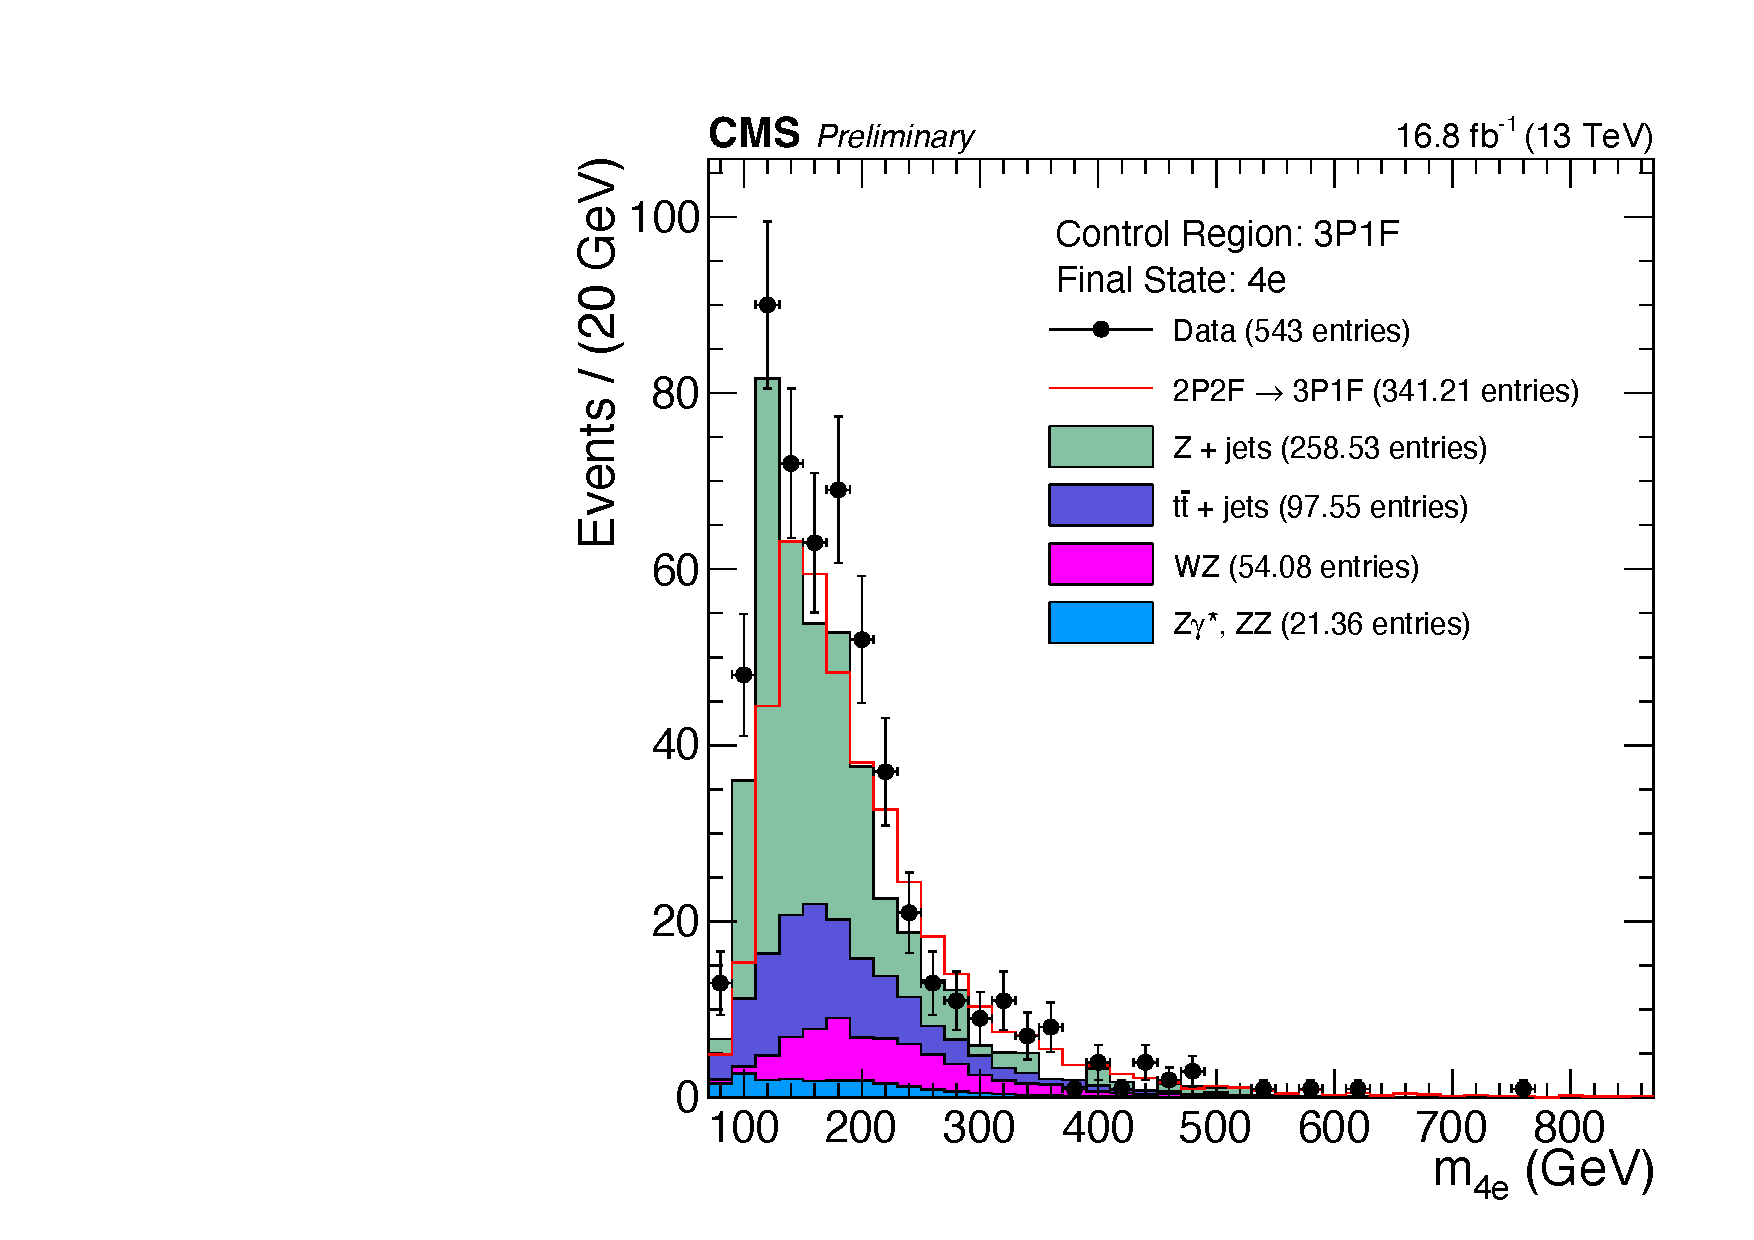
\includegraphics[width=0.48\textwidth]{figures/higgsmassmeas/redbkg/cr/UL2016postVFP_CR_3P1F_4e.pdf}
		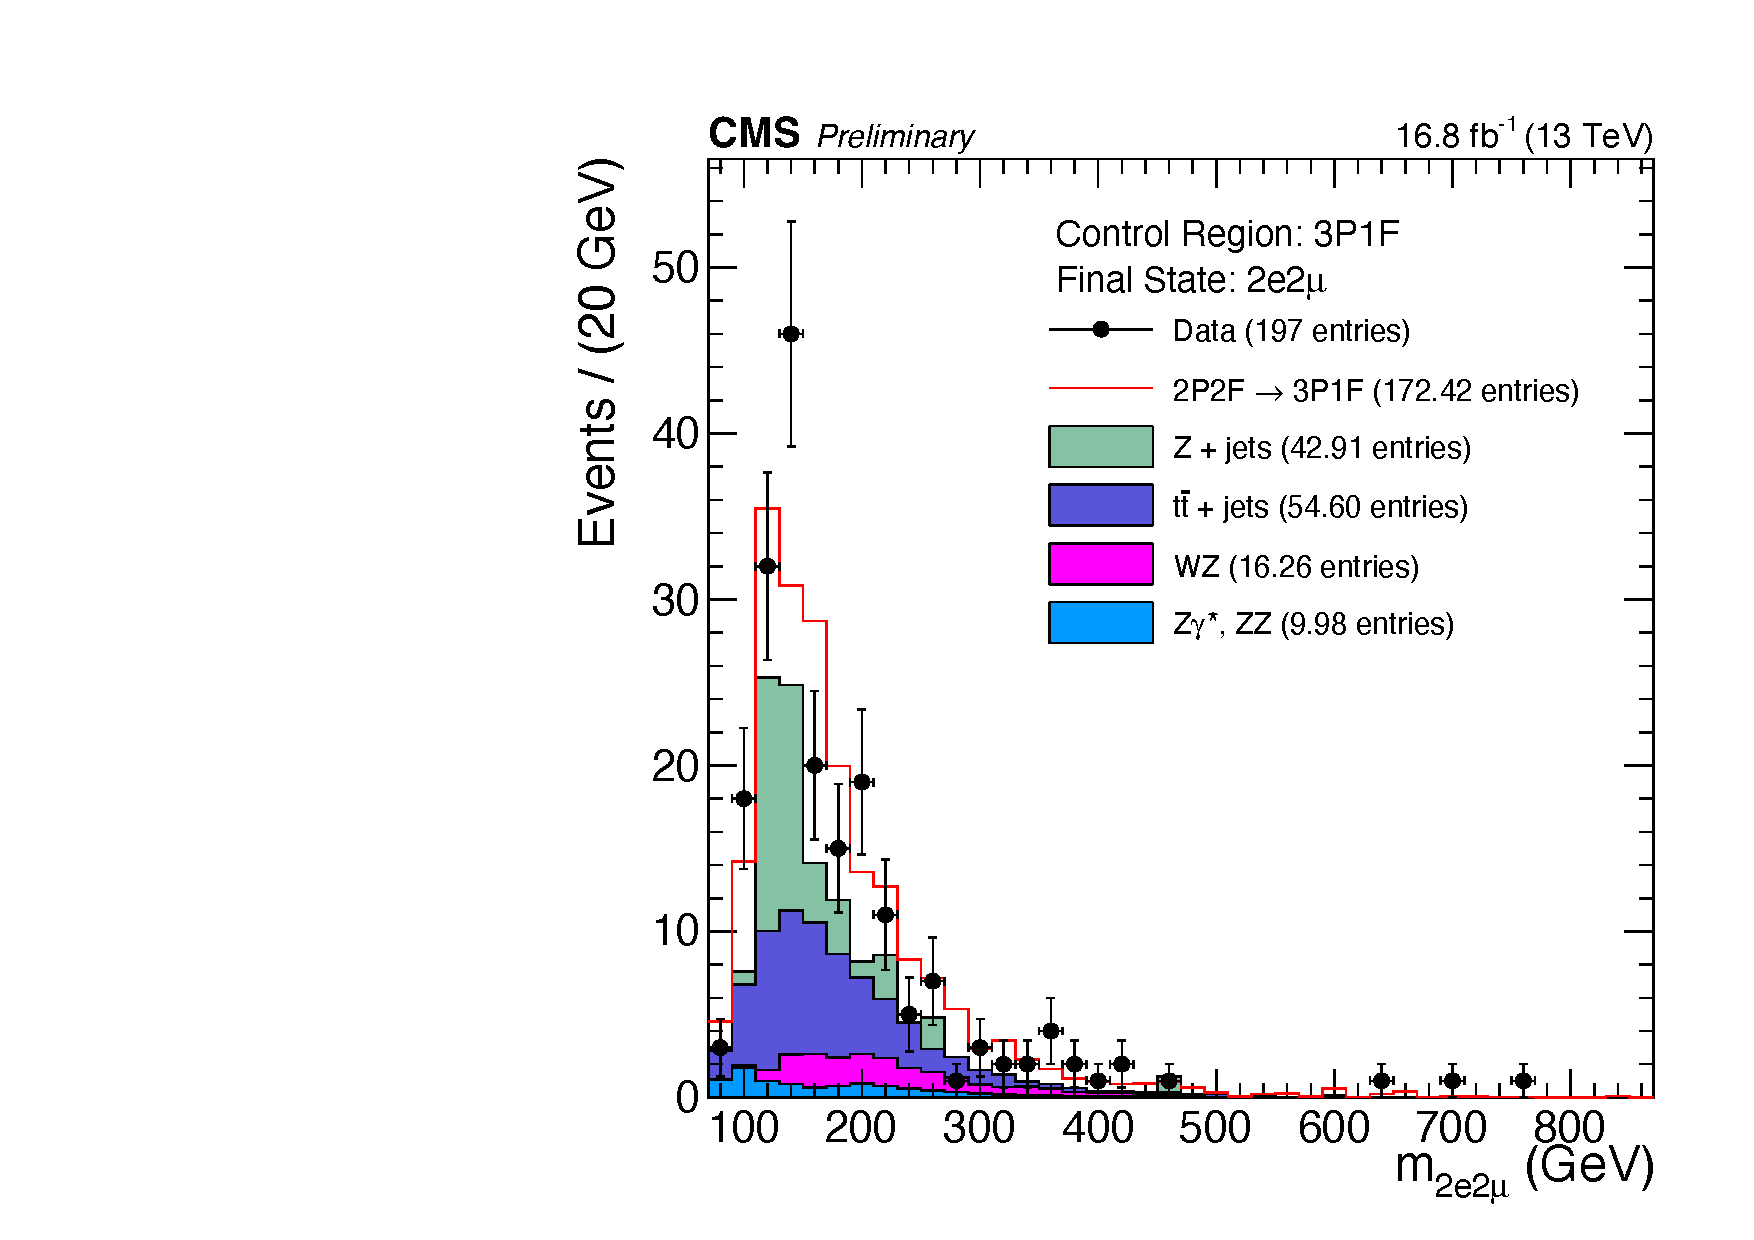
\includegraphics[width=0.48\textwidth]{figures/higgsmassmeas/redbkg/cr/UL2016postVFP_CR_3P1F_2e2mu.pdf}
		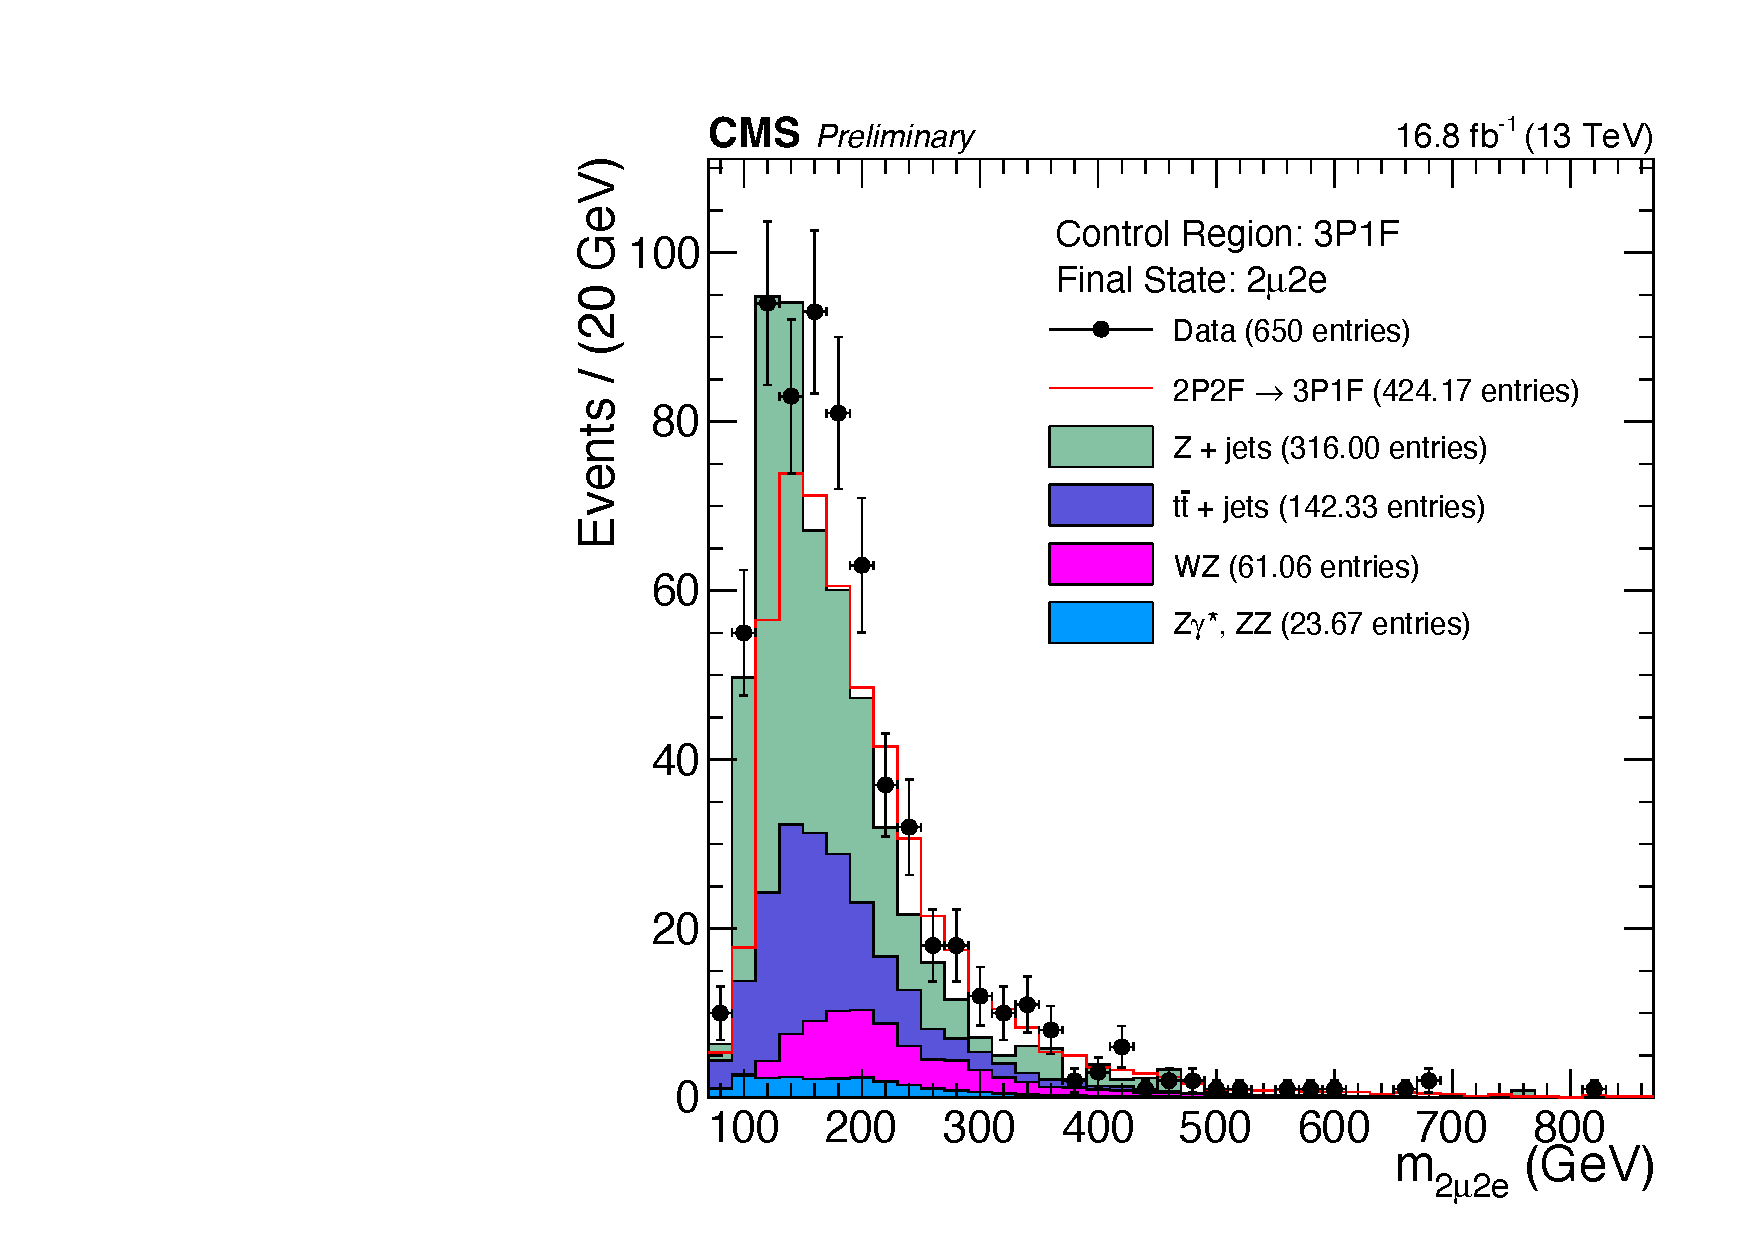
\includegraphics[width=0.48\textwidth]{figures/higgsmassmeas/redbkg/cr/UL2016postVFP_CR_3P1F_2mu2e.pdf}
		\caption{
			Events from 2016 post-VFP UL data that pass 3P1F CR selections (black markers) 
			are compared to the stacked 3P1F distributions of simulated samples
			(\Zplusjets, \ttbarplusjets, \WZ, \ZZ, \Zgammastar)
			and to the predicted contribution of 2-prompt-2-nonprompt-lepton processes to the 3P1F CR (red line).
			This prediction is obtained by making a distribution of all event weights given by Eq.~\ref{eqn:wt_2prto3p1f_simp} and stacking that on top of the WZ and \ZZ distributions.
			The results are split into the $4\ell$ final states:
			$4\mu$ (top left), 4e (top right), 2e2$\mu$ (bottom left), 2$\mu$2e (bottom right).
		}
		\label{cr_plots_3p1f_2016postvfp}
	\end{center}
\end{figure}
\begin{figure}[!htbp]
	\begin{center}
		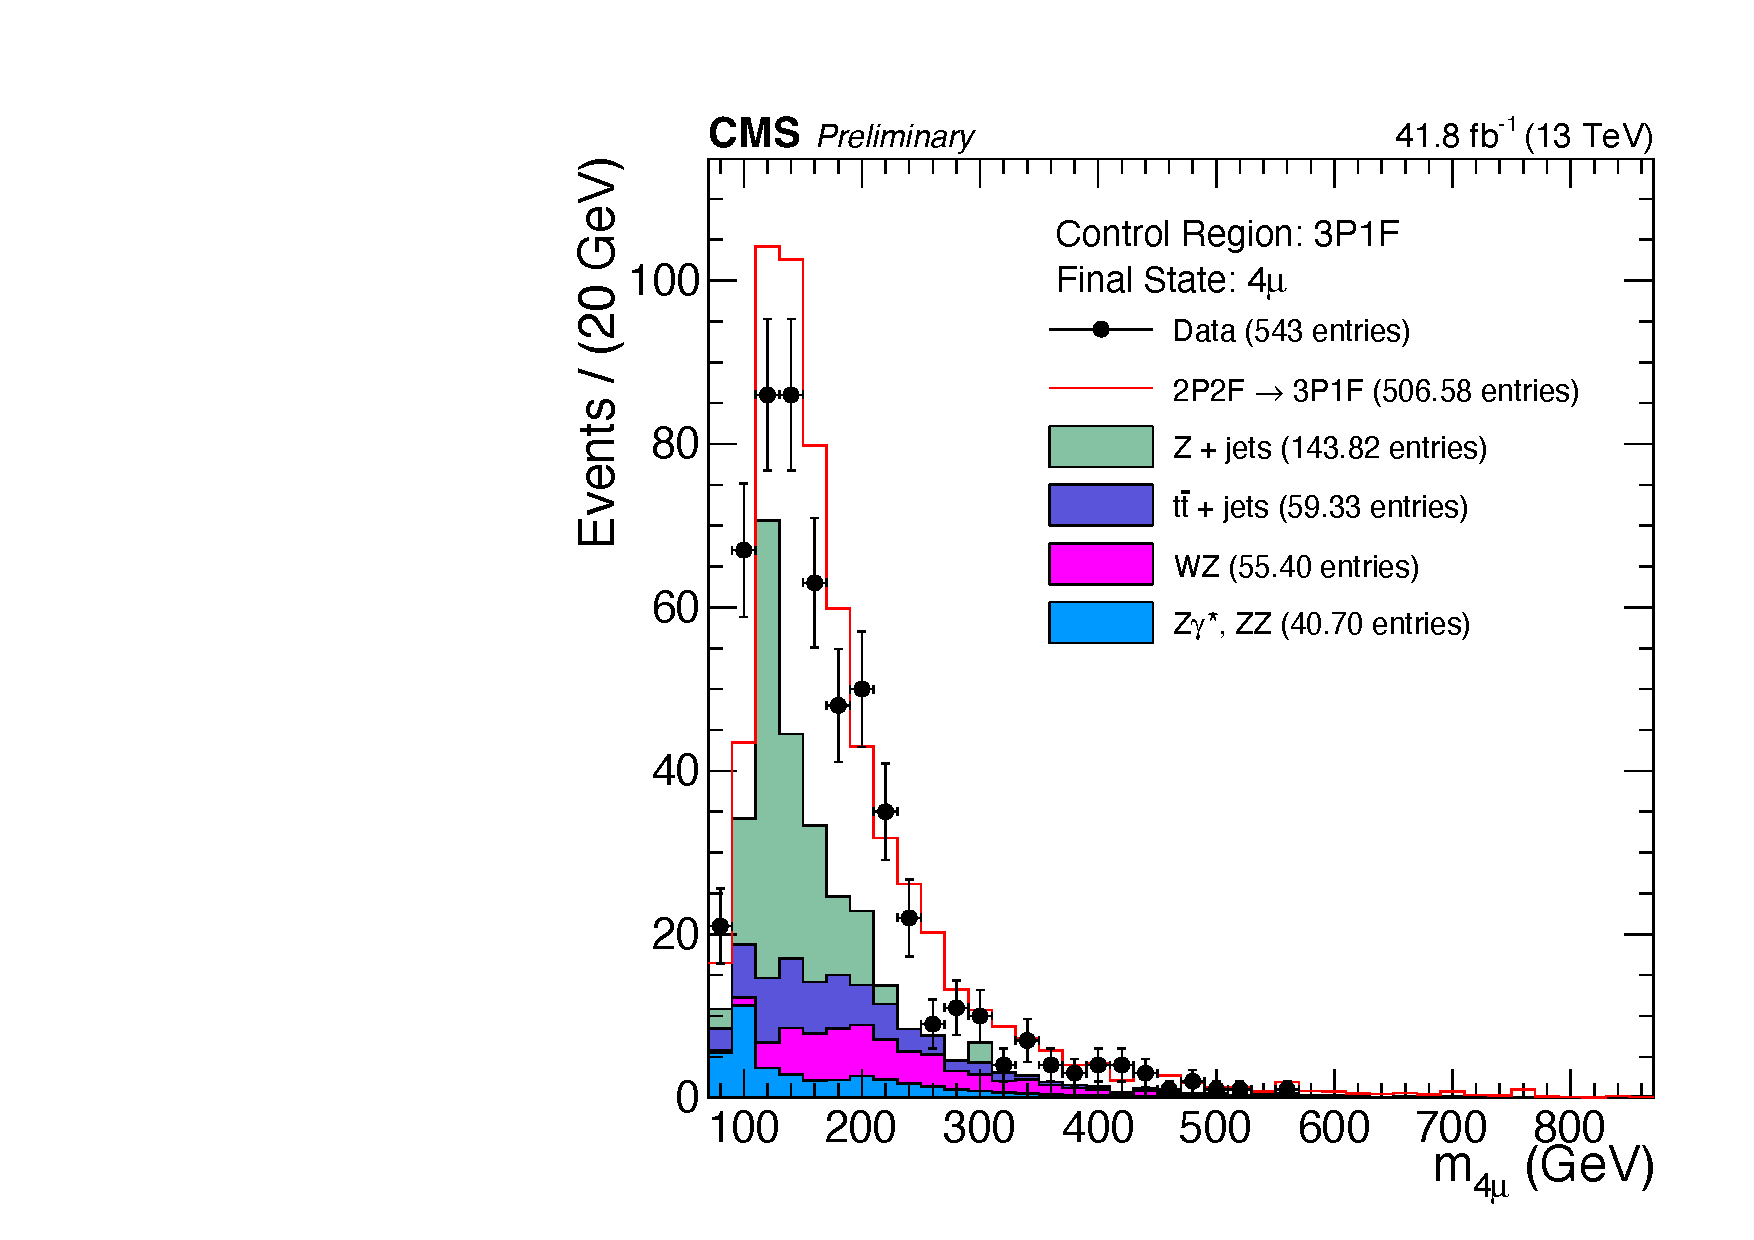
\includegraphics[width=0.48\textwidth]{figures/higgsmassmeas/redbkg/cr/UL2017_CR_3P1F_4mu.pdf}
		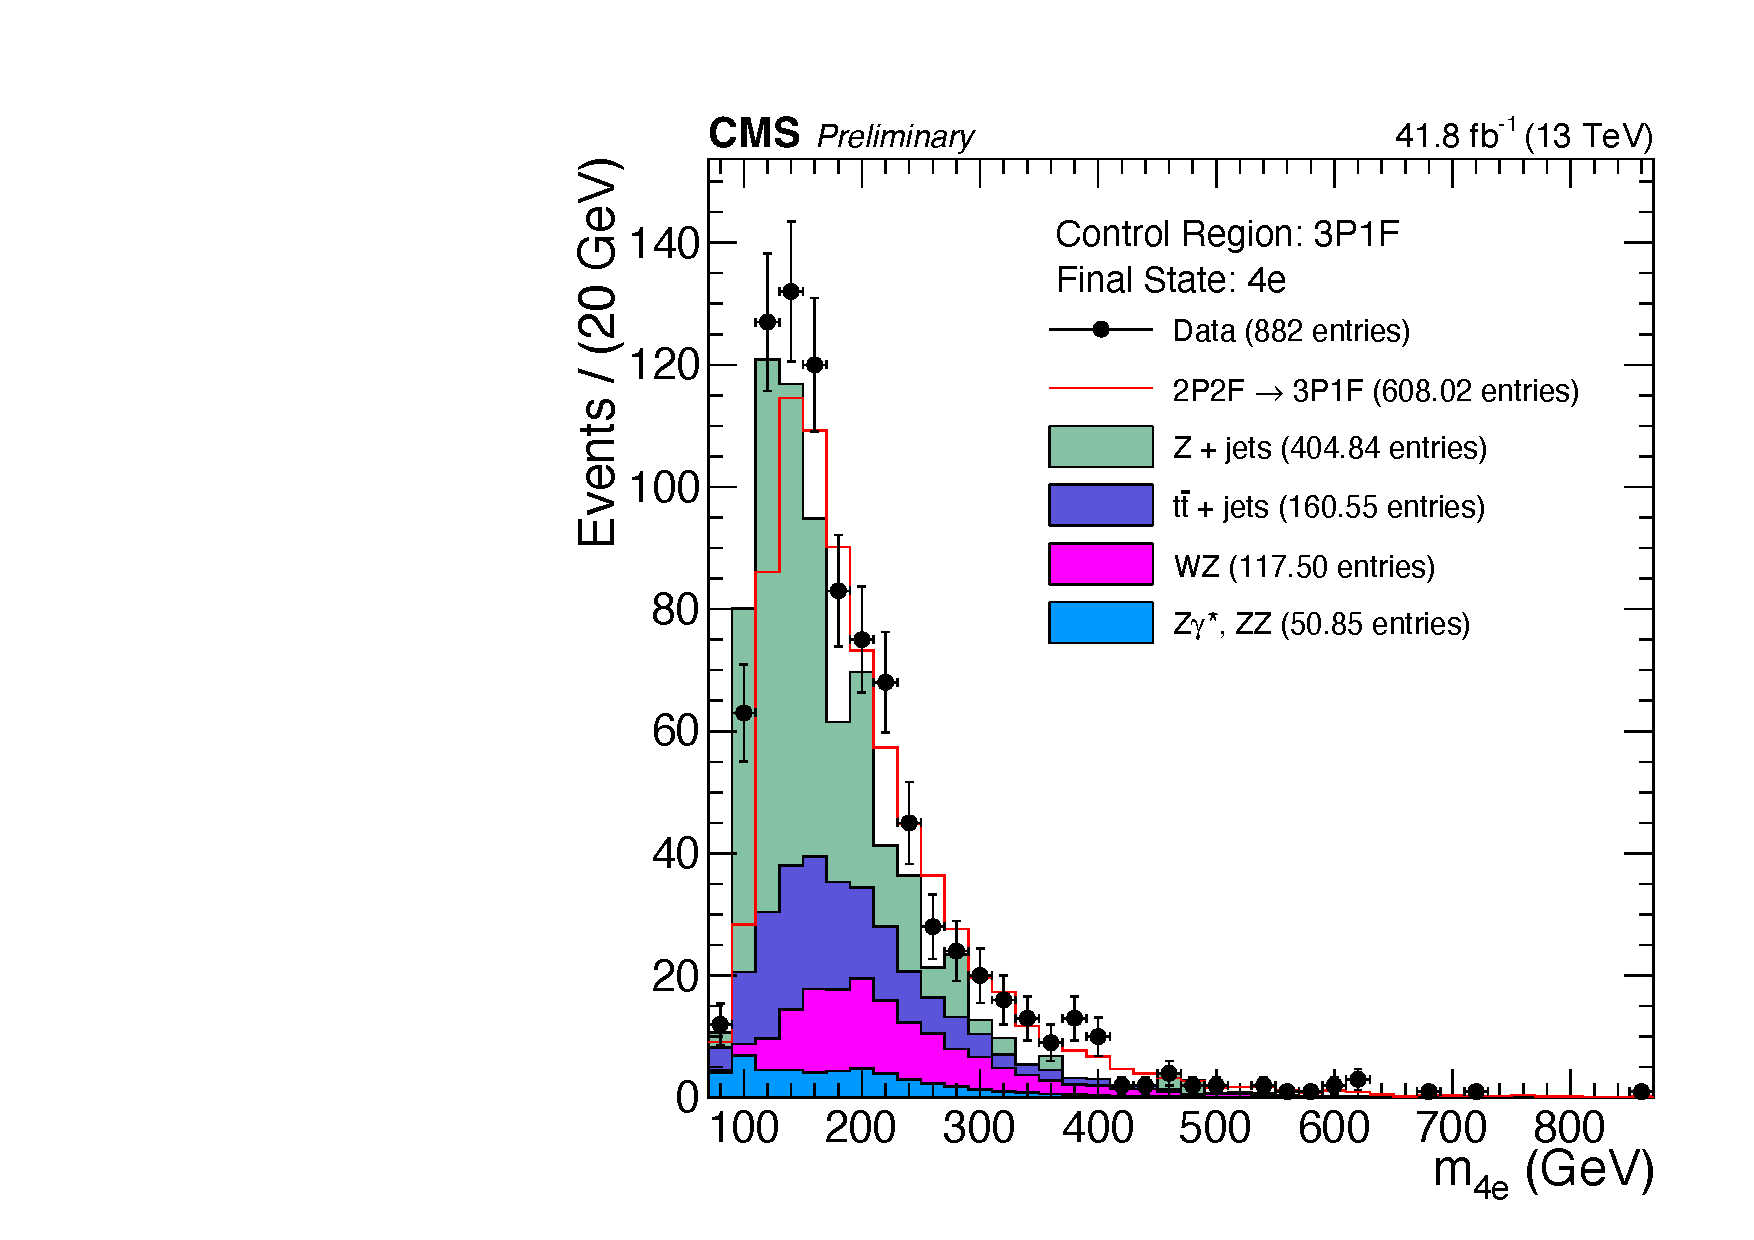
\includegraphics[width=0.48\textwidth]{figures/higgsmassmeas/redbkg/cr/UL2017_CR_3P1F_4e.pdf}
		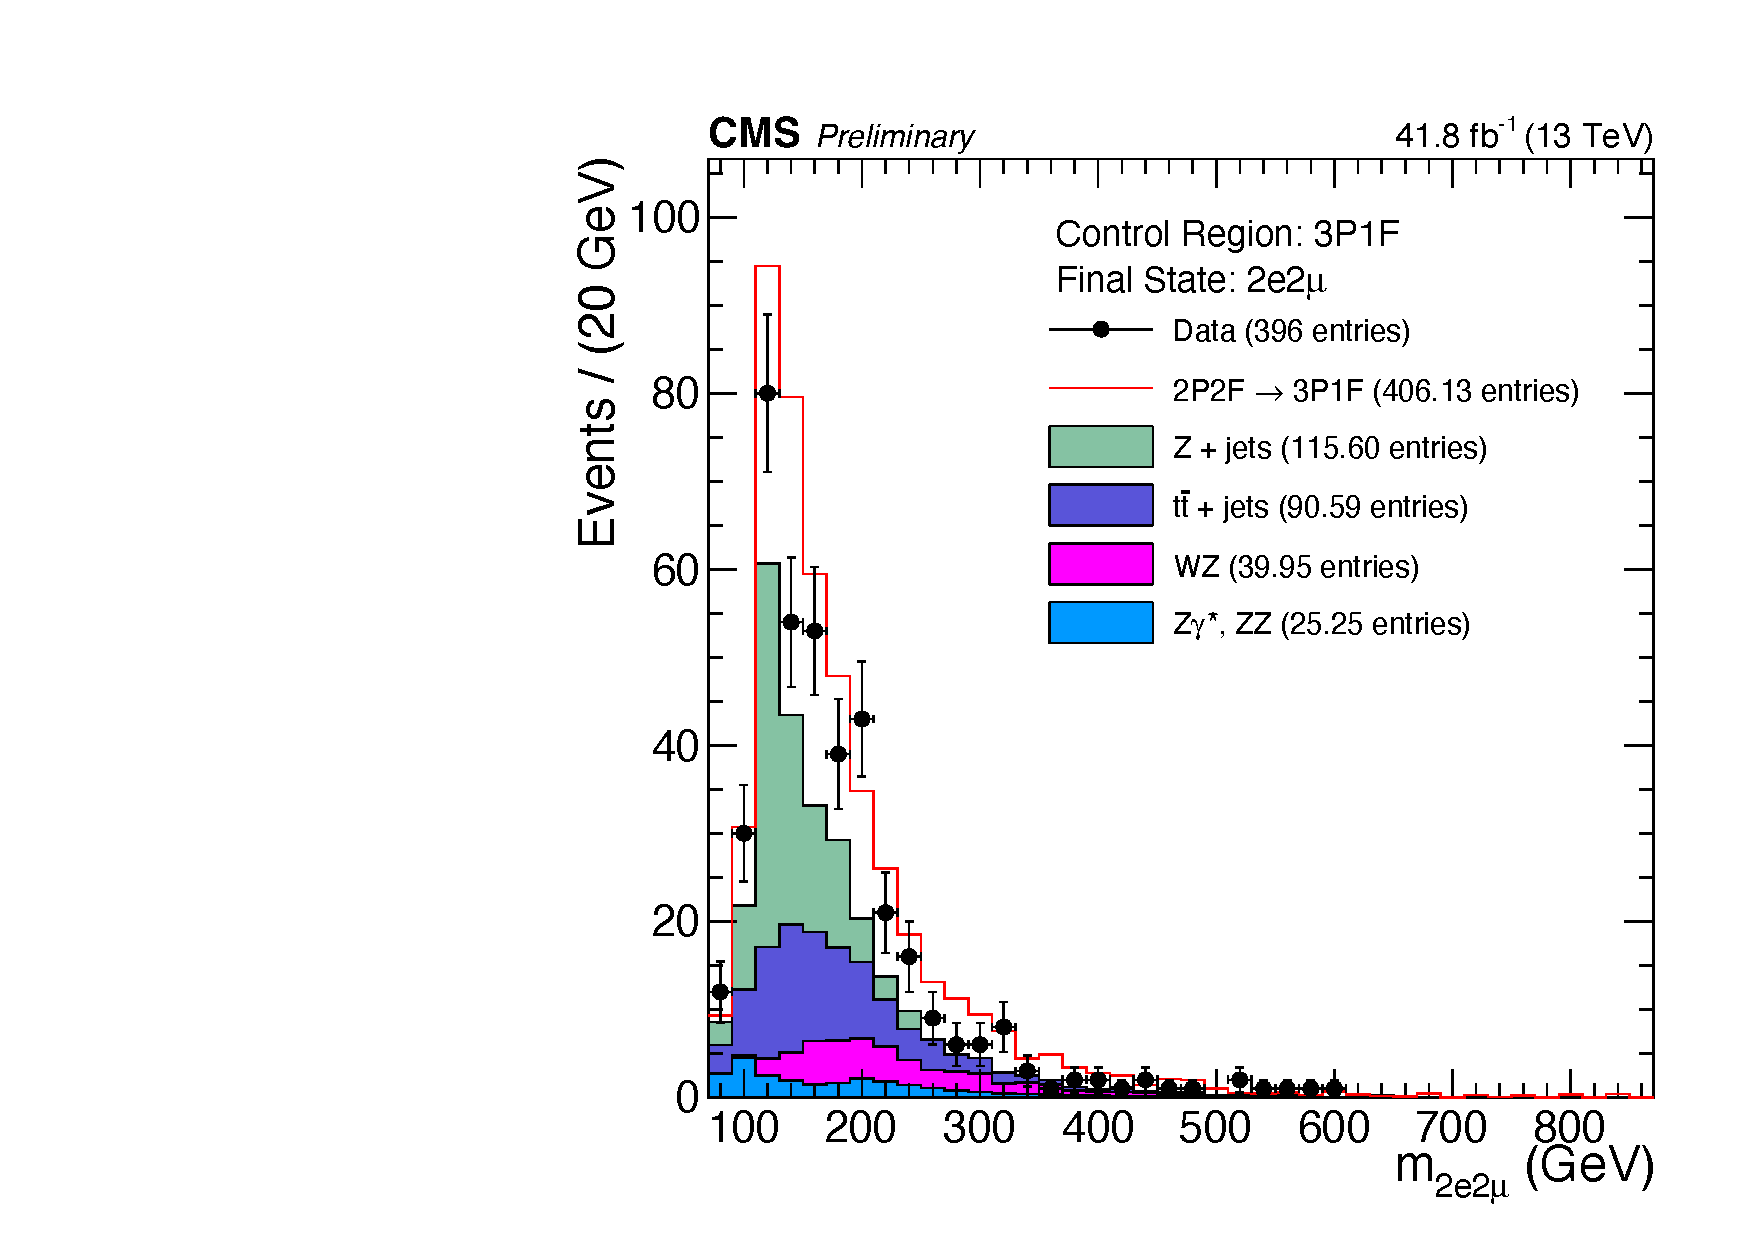
\includegraphics[width=0.48\textwidth]{figures/higgsmassmeas/redbkg/cr/UL2017_CR_3P1F_2e2mu.pdf}
		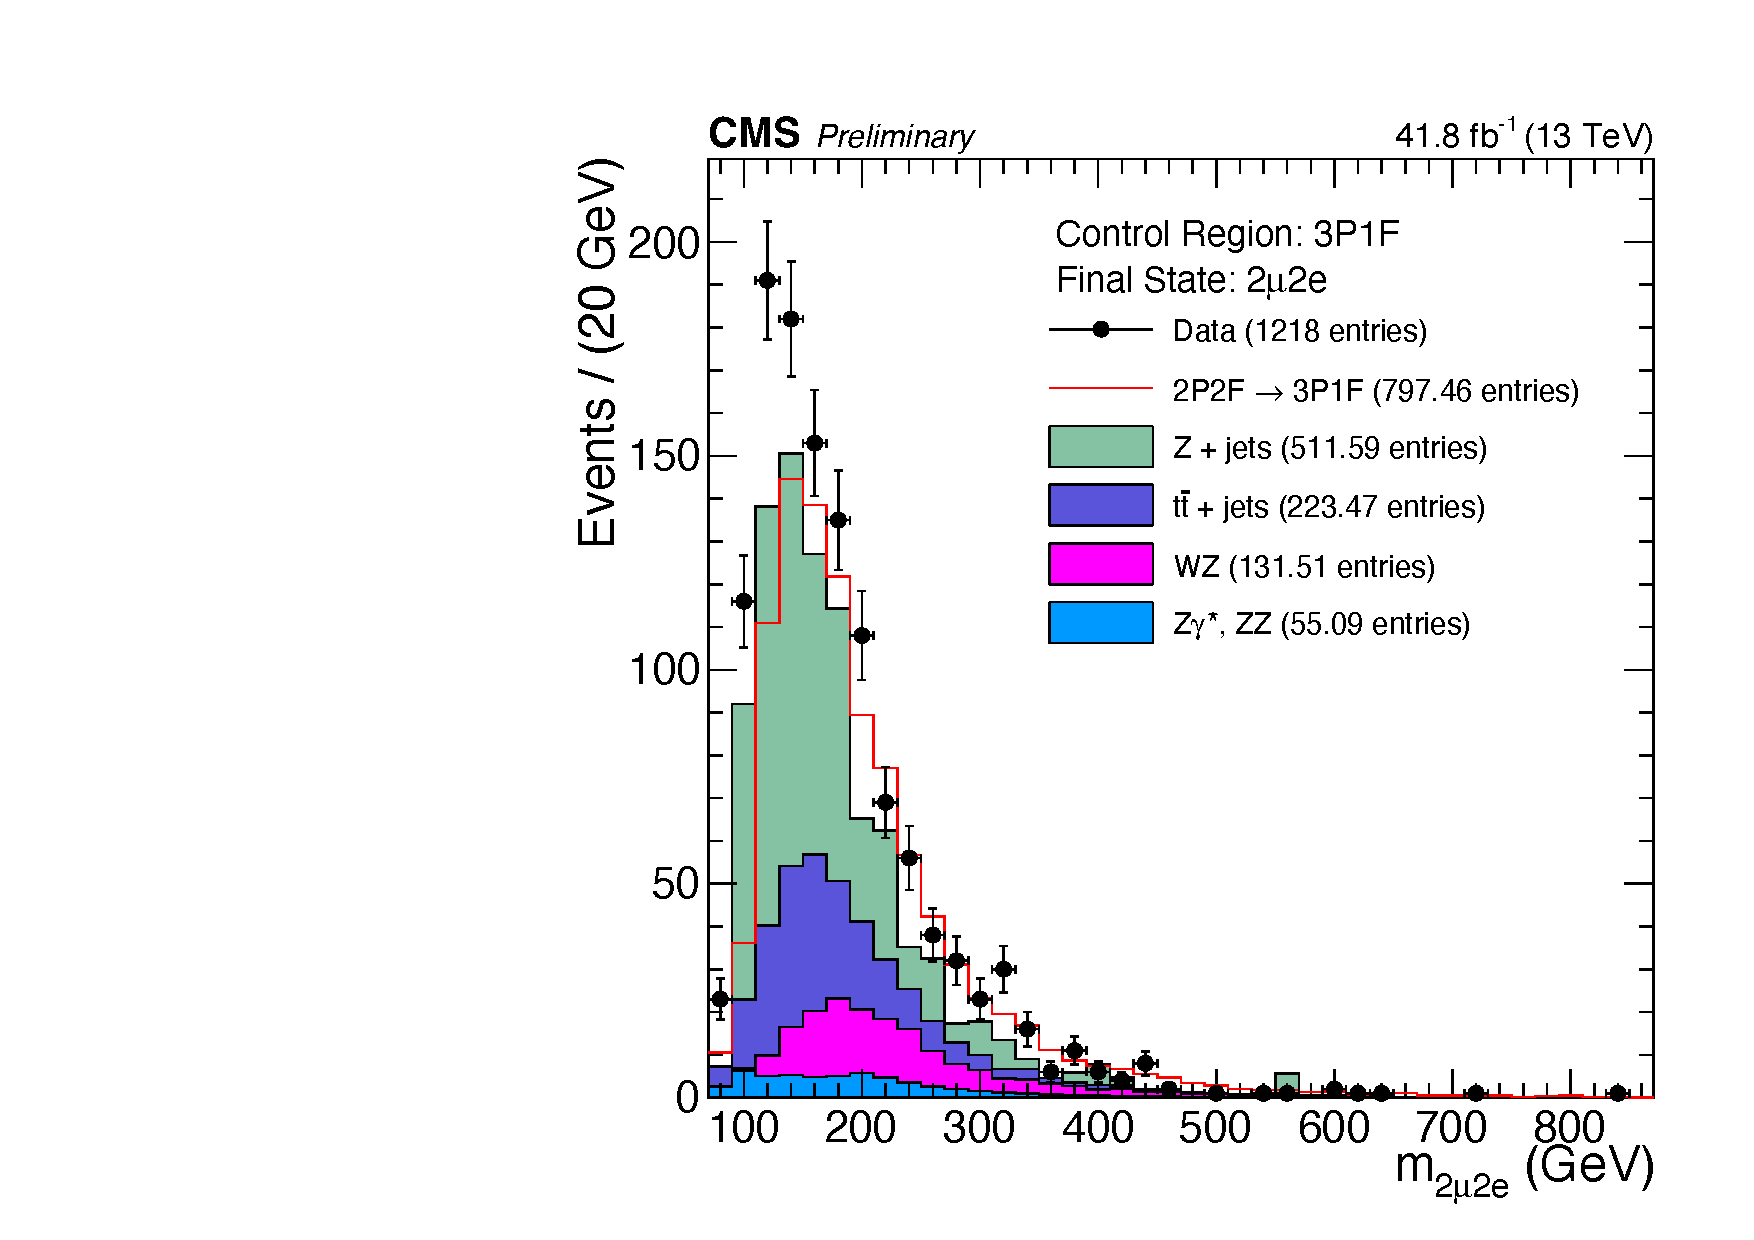
\includegraphics[width=0.48\textwidth]{figures/higgsmassmeas/redbkg/cr/UL2017_CR_3P1F_2mu2e.pdf}
		\caption{
			Events from 2017 UL data that pass 3P1F CR selections (black markers) 
			are compared to the stacked 3P1F distributions of simulated samples
			(\Zplusjets, \ttbarplusjets, \WZ, \ZZ, \Zgammastar)
			and to the predicted contribution of 2-prompt-2-nonprompt-lepton processes to the 3P1F CR (red line).
			This prediction is obtained by making a distribution of all event weights given by Eq.~\ref{eqn:wt_2prto3p1f_simp} and stacking that on top of the WZ and \ZZ distributions.
			The results are split into the $4\ell$ final states:
			$4\mu$ (top left), 4e (top right), 2e2$\mu$ (bottom left), 2$\mu$2e (bottom right).
		}
		\label{cr_plots_3p1f_2017}
	\end{center}
\end{figure}
\begin{figure}[!htbp]
	\begin{center}
		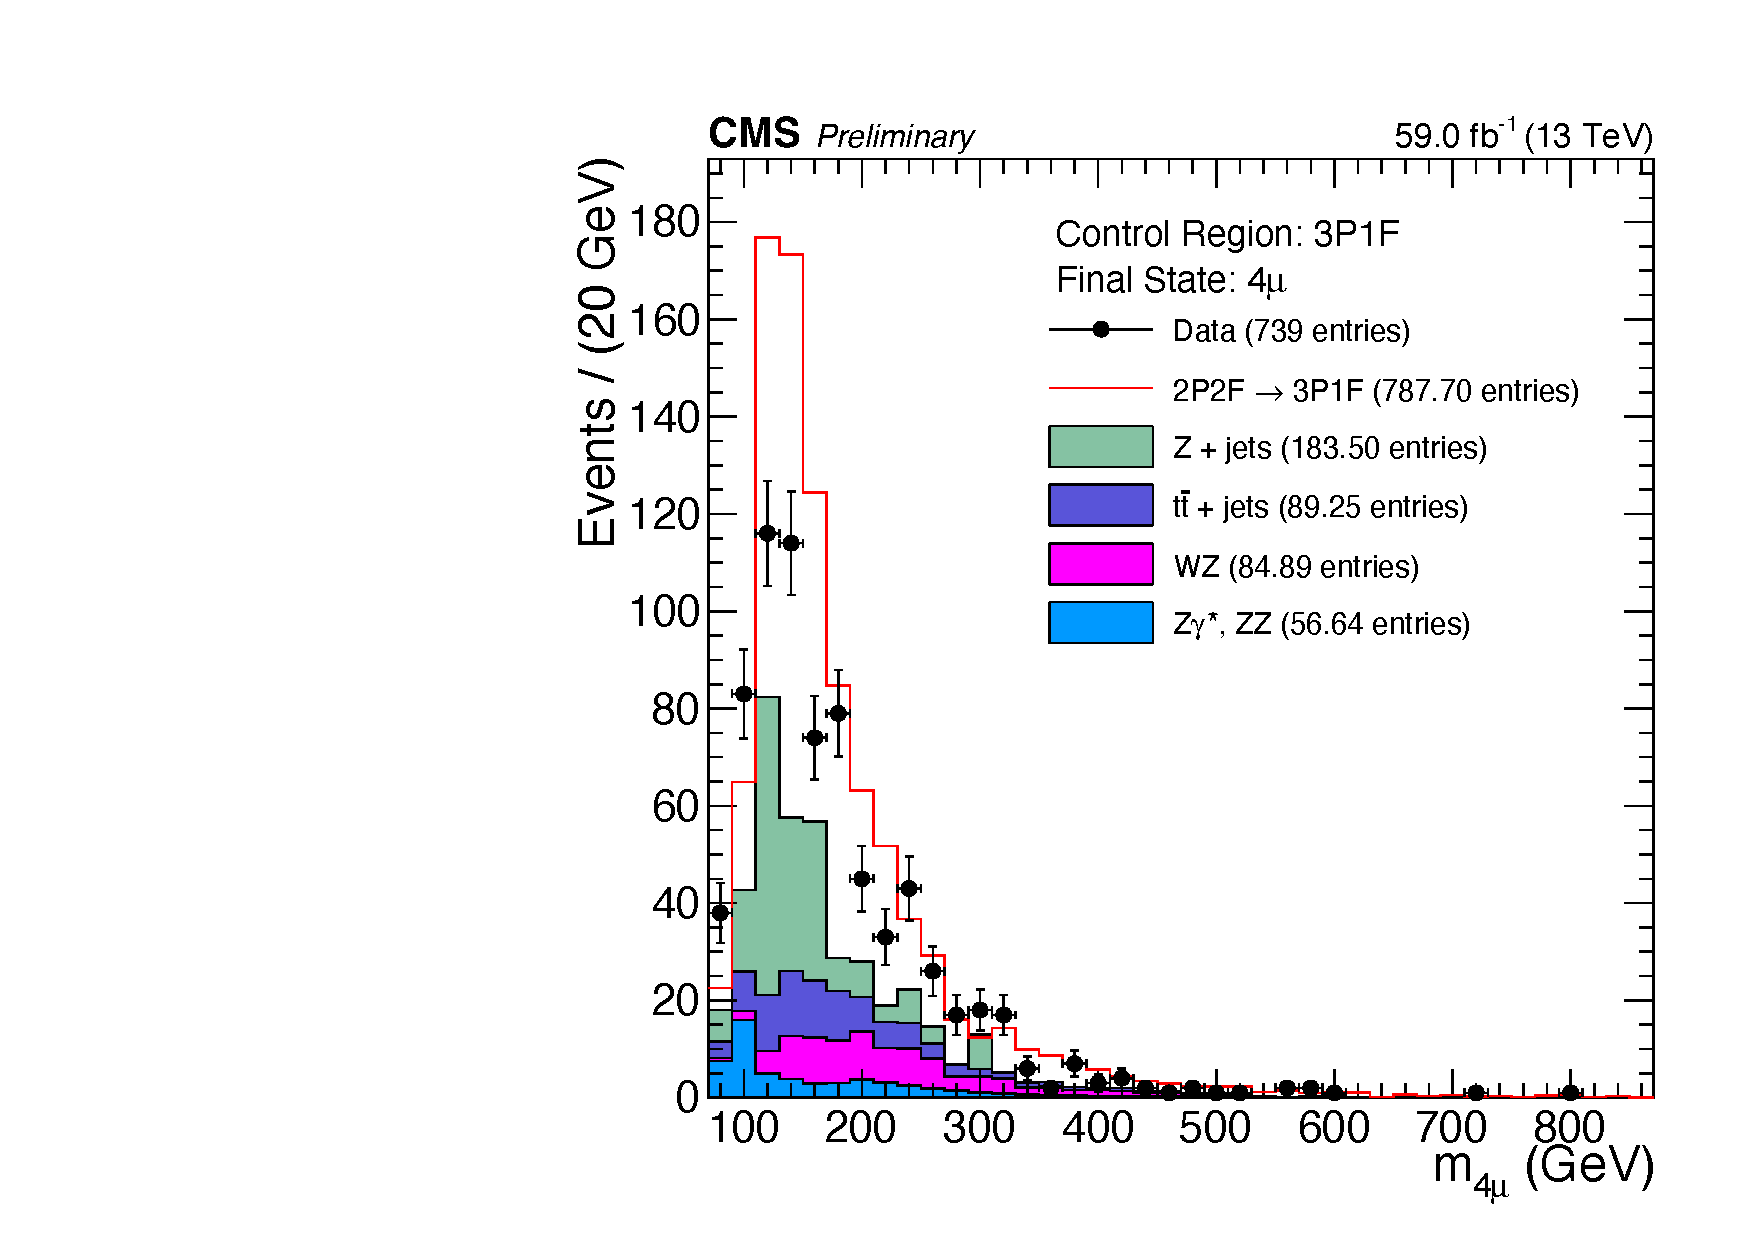
\includegraphics[width=0.48\textwidth]{figures/higgsmassmeas/redbkg/cr/UL2018_CR_3P1F_4mu.pdf}
		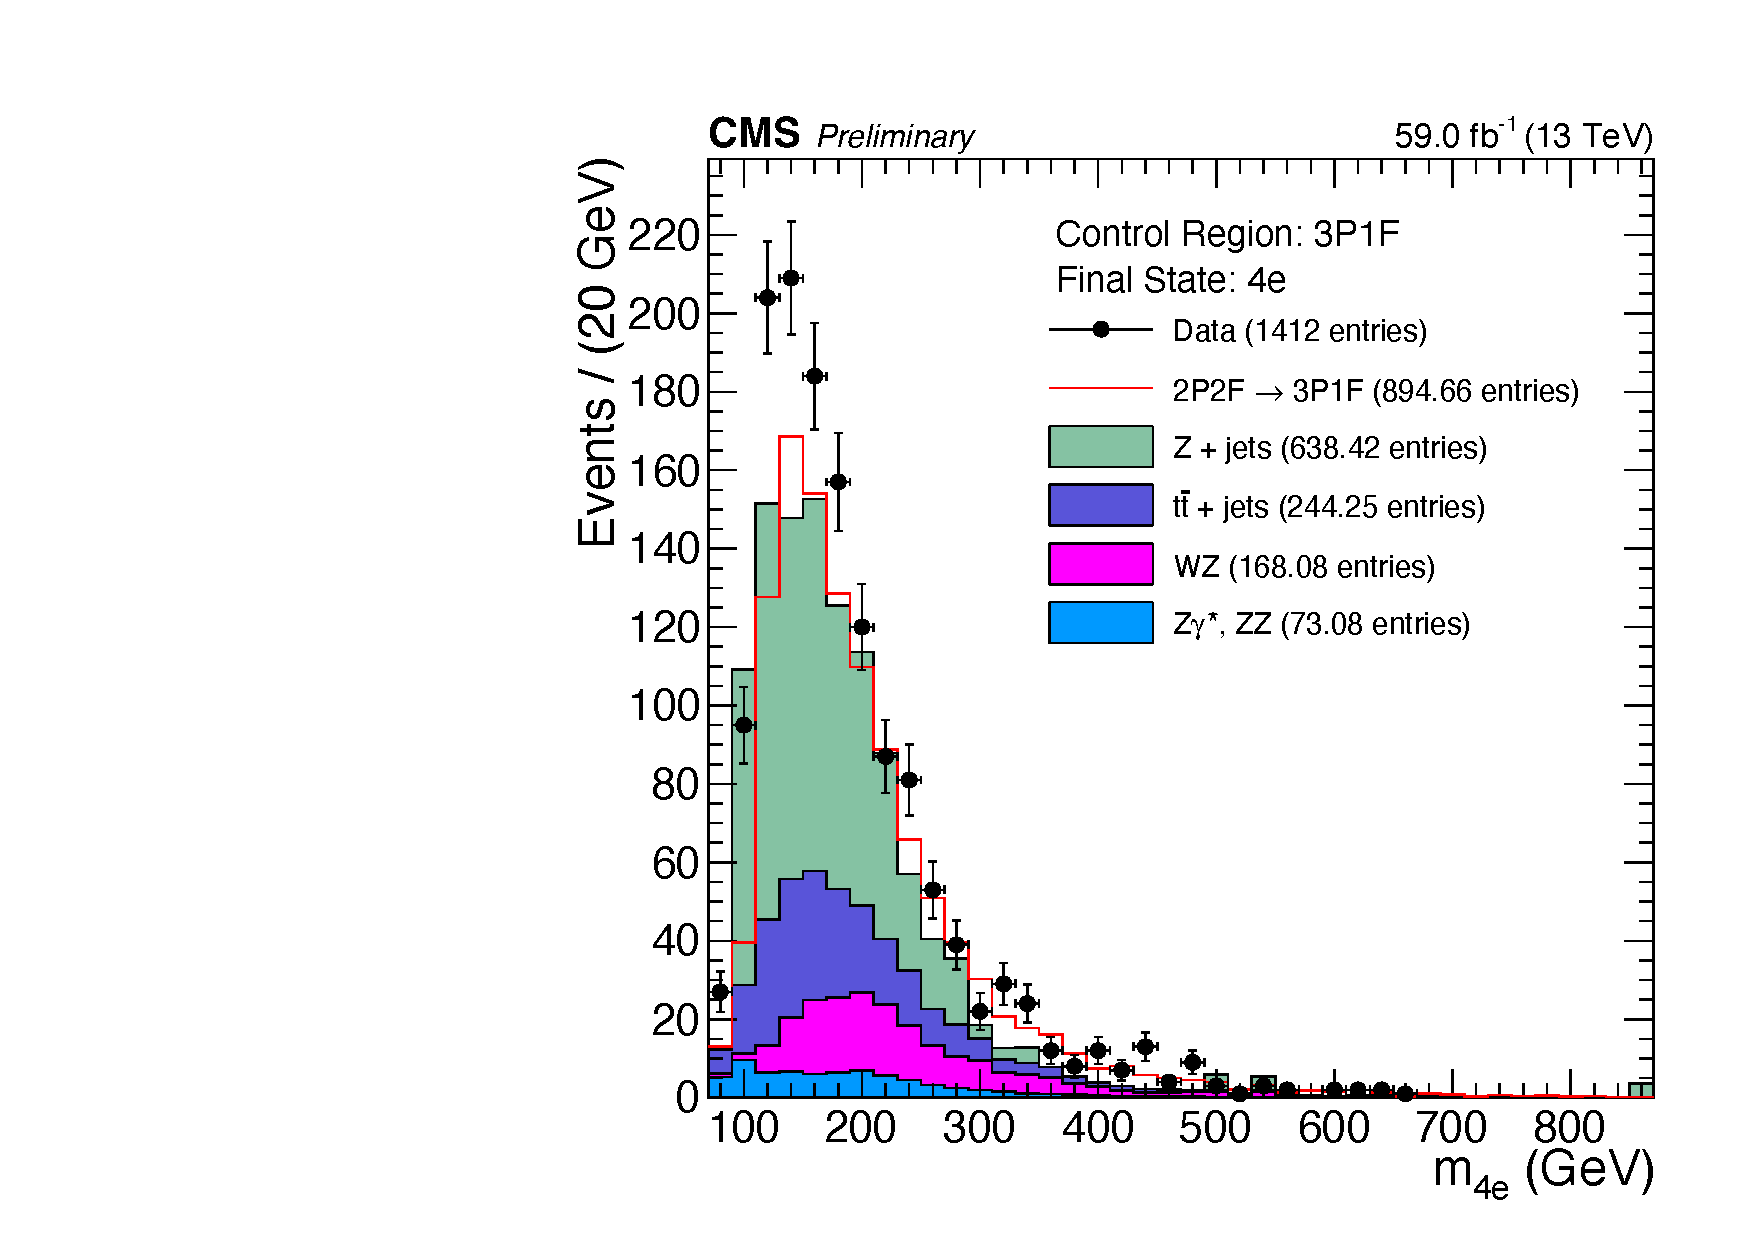
\includegraphics[width=0.48\textwidth]{figures/higgsmassmeas/redbkg/cr/UL2018_CR_3P1F_4e.pdf}
		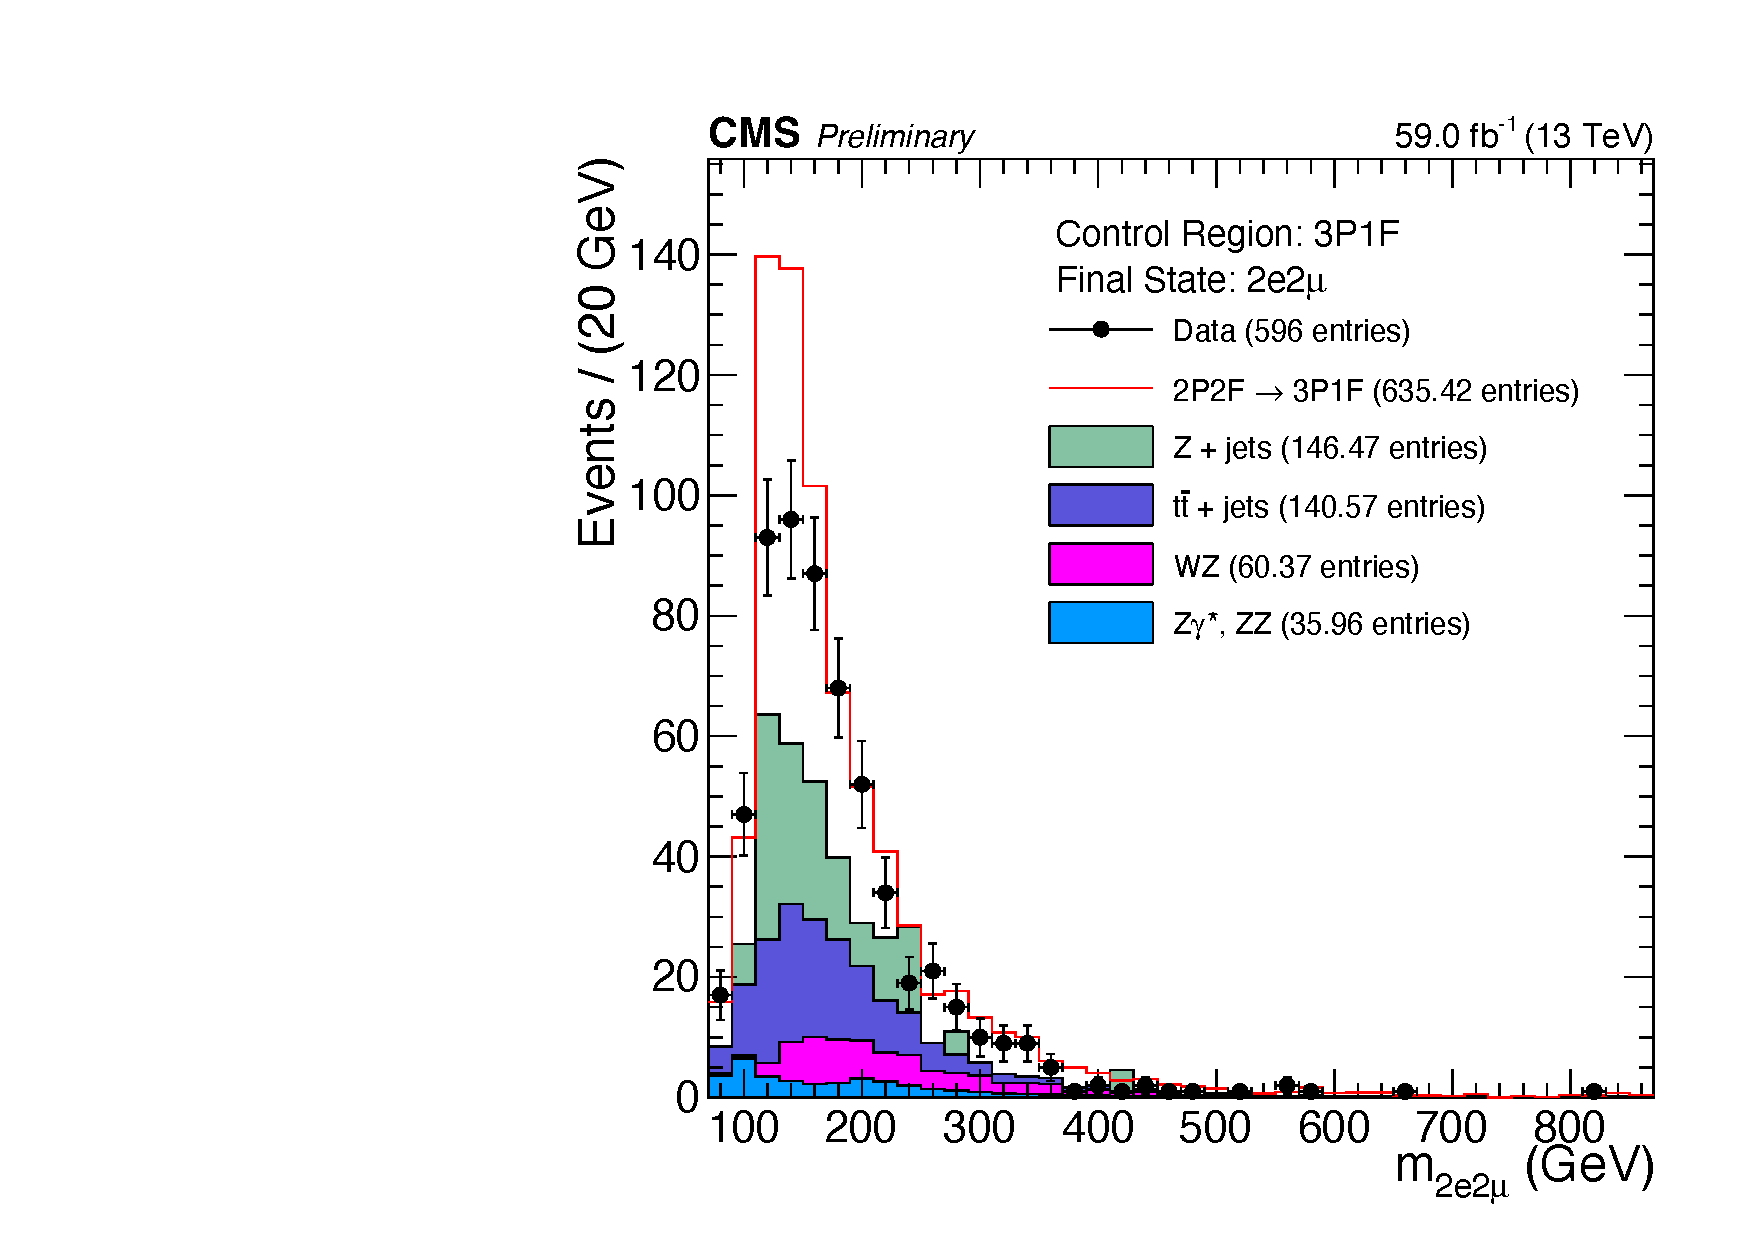
\includegraphics[width=0.48\textwidth]{figures/higgsmassmeas/redbkg/cr/UL2018_CR_3P1F_2e2mu.pdf}
		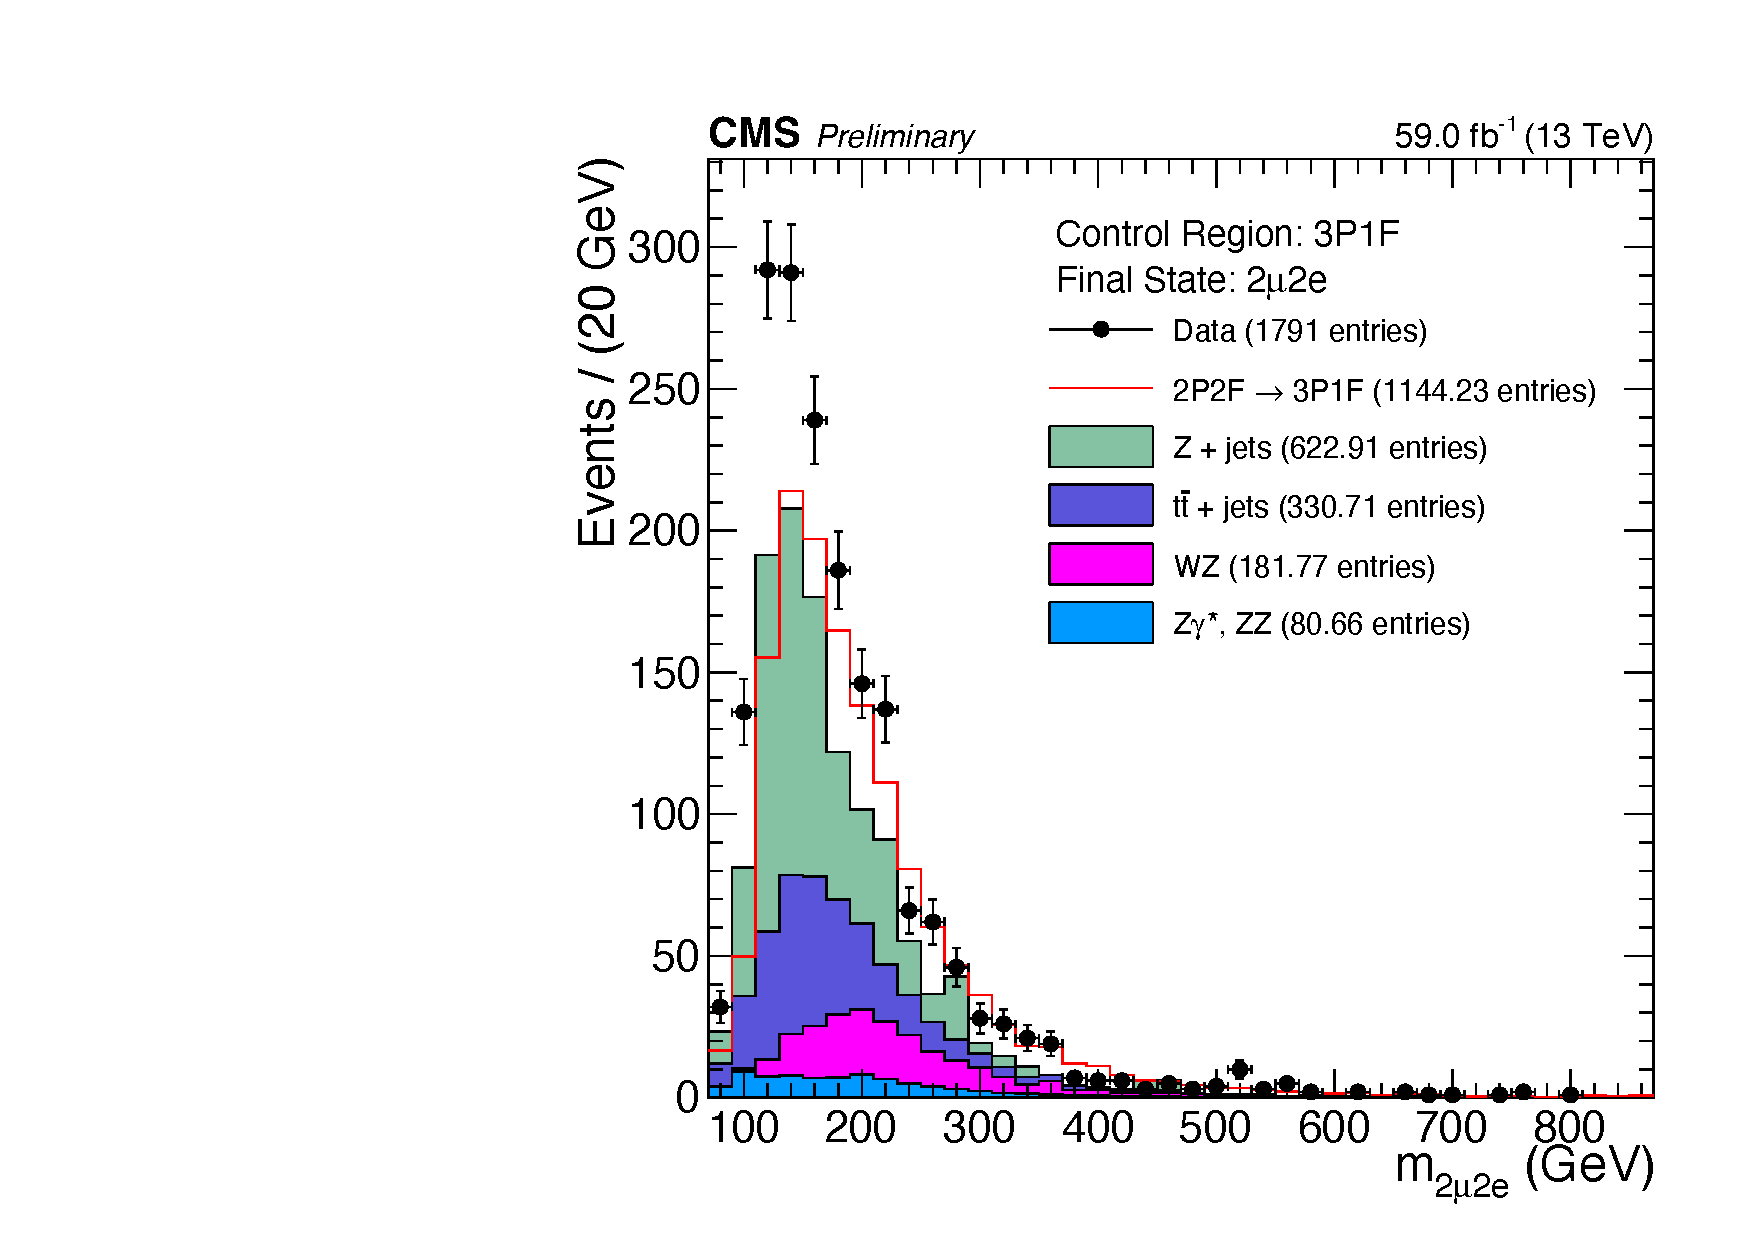
\includegraphics[width=0.48\textwidth]{figures/higgsmassmeas/redbkg/cr/UL2018_CR_3P1F_2mu2e.pdf}
		\caption{
			Events from 2018 UL data that pass 3P1F CR selections (black markers) 
			are compared to the stacked 3P1F distributions of simulated samples
			(\Zplusjets, \ttbarplusjets, \WZ, \ZZ, \Zgammastar)
			and to the predicted contribution of 2-prompt-2-nonprompt-lepton processes to the 3P1F CR (red line).
			This prediction is obtained by making a distribution of all event weights given by Eq.~\ref{eqn:wt_2prto3p1f_simp} and stacking that on top of the WZ and \ZZ distributions.
			The results are split into the $4\ell$ final states:
			$4\mu$ (top left), 4e (top right), 2e2$\mu$ (bottom left), 2$\mu$2e (bottom right).
		}
		\label{cr_plots_3p1f_2018}
	\end{center}
\end{figure}

% \subsubsection{Tight-to-loose lepton rates}
\subsubsection{Lepton misidentification rate measurement}
\label{sec:fr_evtsel}
As mentioned in Section~\ref{sec:redbkg}, the lepton misidentification rate ($f$) is the probability that a nonprompt lepton will pass tight selections (PTS).
The value $f$ is a function of the flavor ($\ell = \text{e}, \mu$), \pt, and $\eta$ of a lepton.
The misidentification rate is calculated by simply counting the number of nonprompt PTS leptons $\left( N^{\mathrm{np}}_{\mathrm{P}} \right)$ that enter a particular $\ell, \pt, \abseta$ bin compared to the total number of loose probe leptons $\left( N^{\mathrm{np}}_{\mathrm{L}} \right)$ in the same bin:
\begin{equation}
	\label{eqn:fr_calc}
	f\left( \ell, \abseta, \pt \right) = 
	\frac{
		N^{\mathrm{np}}_{\mathrm{P}}
		}{
		N^{\mathrm{np}}_{\mathrm{L}}
		}.
\end{equation}
The $\pt^e$ bin edges are [5--10--20--30--40--50--80]\GeV and the $\pt^{\mu}$ bin edges are [5--7--10--20--30--40--50--80]\GeV.
% Since the 2P2F, 3P1F, and 4P regions all contain an unreliable
The nonprompt leptons used to measure $f$ are taken from events in data with a signature like that of \ZplusL, where Z is a Z boson and \looselep is a loose lepton ($\Pe, \mu$).
By construction, this region of events is orthogonal to the 2P2F, 3P1F, and 4P regions, and provides a clean source of \looselep.
The loose lepton, whose selection is defined in Sections~\ref{sec:el_sel} and~\ref{sec:mu_sel}, is also called the \emph{probe} lepton.
The probe lepton is either a PTS or FTS lepton and is counted towards both the numerator and denominator of Eq.~\ref{eqn:fr_calc}. 

Events are selected that satisfy the following criteria:
\begin{itemize}
	\item The event has exactly 3 leptons.
	\item The event contains $\MET < 25$\GeV.
	\item Two of the leptons form a Z candidate. A Z candidate is formed when:
	\begin{itemize}
		\item The lepton pair is OSSF.
		\item Both leptons PTS.
		\item The leading lepton has $\pt > 20\GeV$.
		\item The subleading lepton has $\pt > 10\GeV$.
		\item The lepton pair satisfies $\left| \mll - m_{\PZ_{\text{PDG}}} \right| < 7\GeV$.
	\end{itemize}
	\item The third and final lepton is loose (\ie either a PTS or FTS lepton).
	\item Suppress QCD processes: probe lepton and OS lepton from Z have $\mll > 4\GeV$.
\end{itemize}

The calculation of $f$ requires that \looselep is a nonprompt lepton but since data events were used, this may not be the case.
For example, the decay of \WZ produces 3 prompt leptons and so this contribution must be subtracted.
Thus, the number of expected prompt probe leptons from \WZ events is subtracted from both the numerator and denominator in Eq.~\ref{eqn:fr_calc} for each $\ell, \pt, \abseta$ bin.
The final misidentification rates used in the OS Method for electrons and muons are shown in Figures~\ref{fr_plots_el} and~\ref{fr_plots_mu} using 2016--2018 UL data.
\begin{figure}[!htbp]
	\begin{center}
		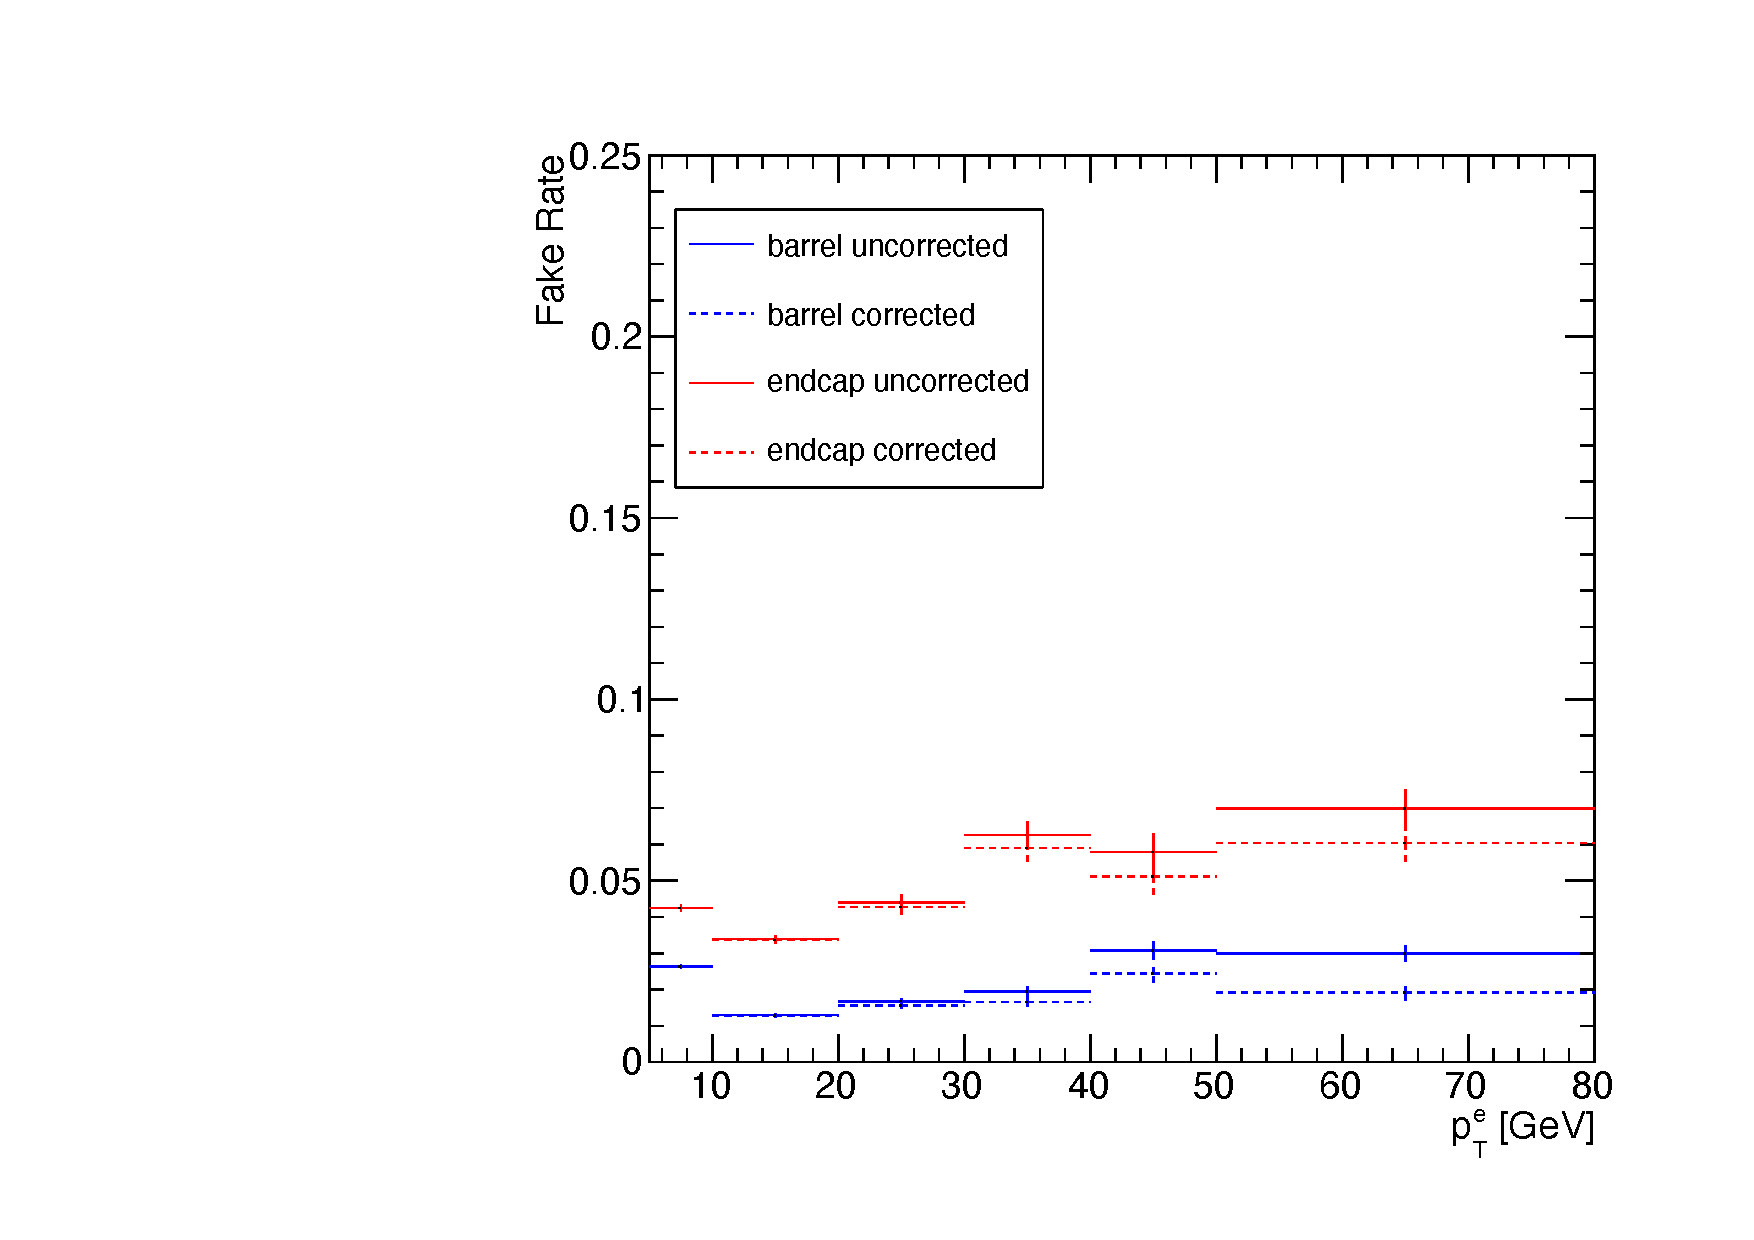
\includegraphics[width=0.48\textwidth]{figures/higgsmassmeas/redbkg/fr/fakerates_UL2016preVFP_el_yaxis_full.pdf}
		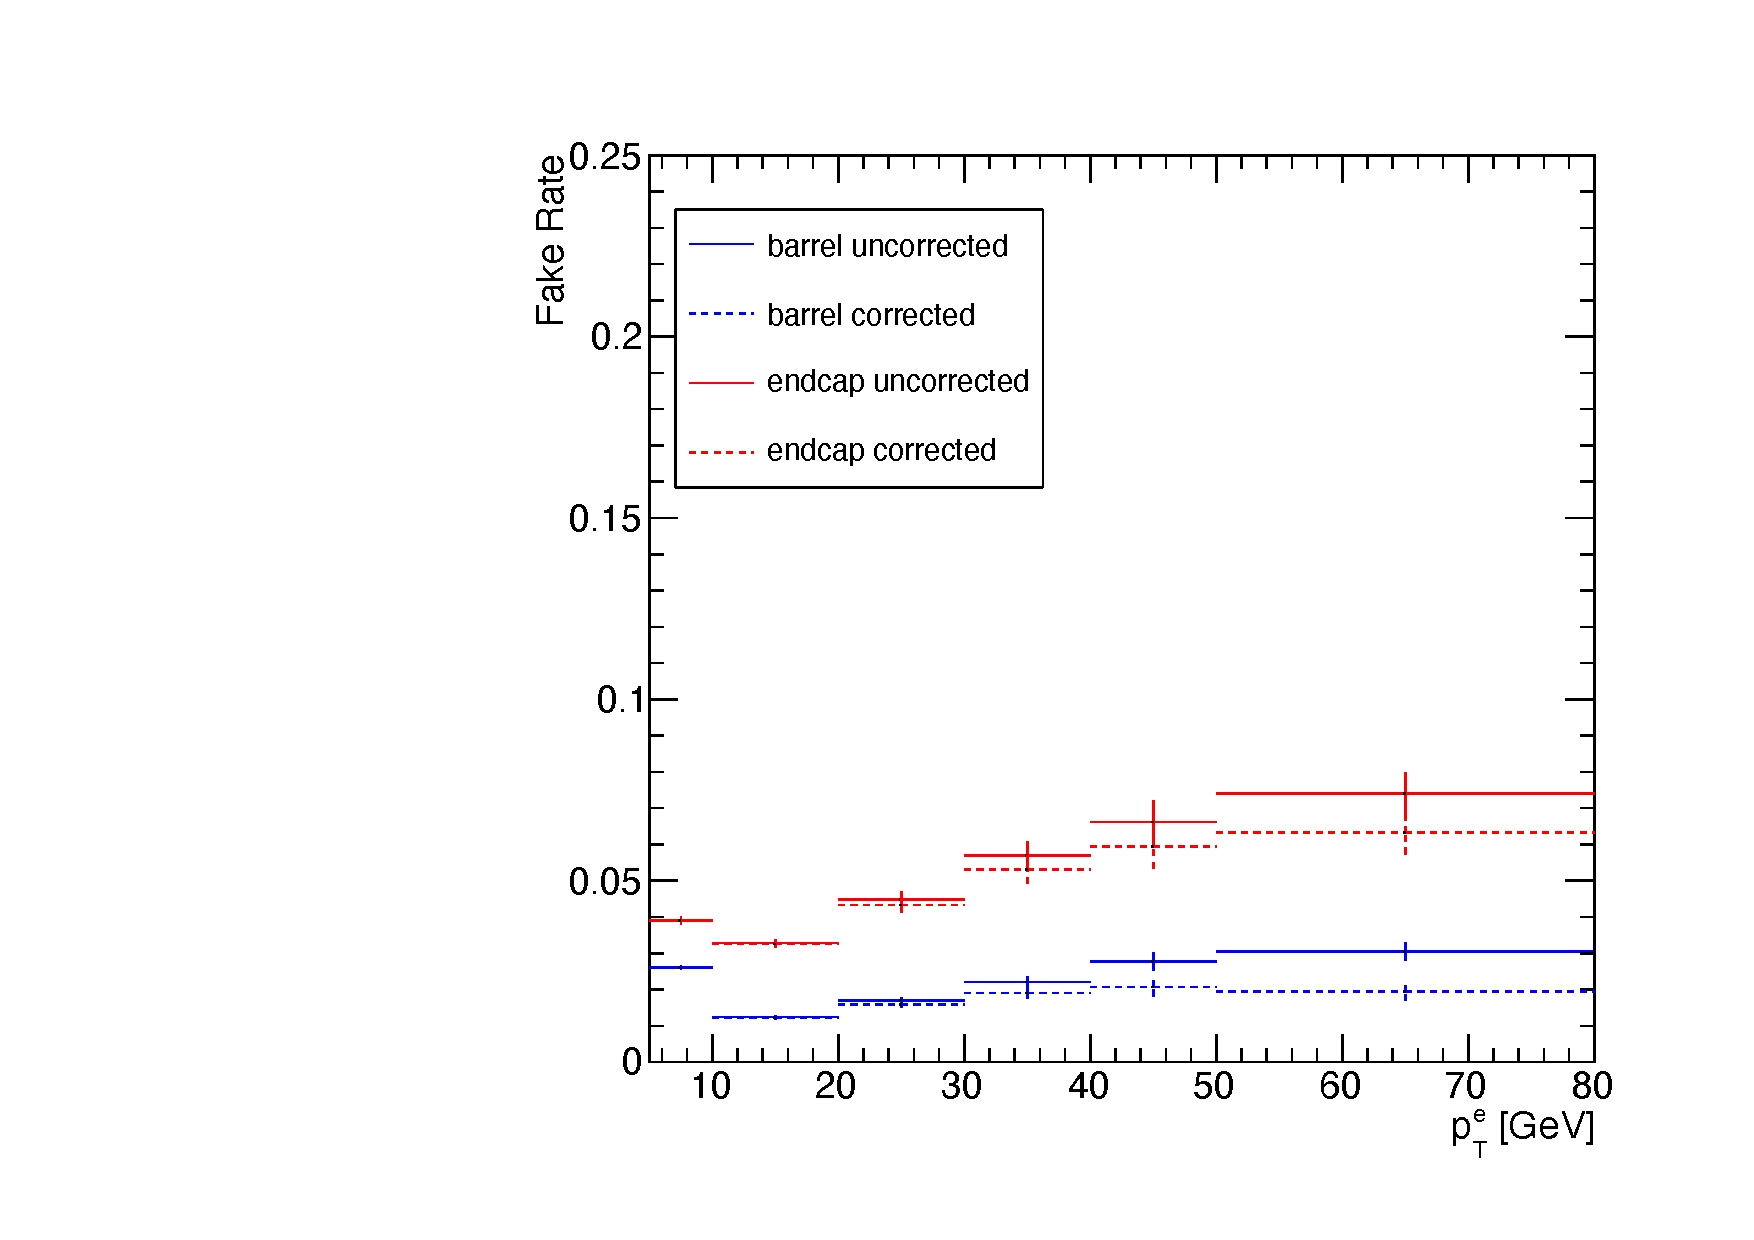
\includegraphics[width=0.48\textwidth]{figures/higgsmassmeas/redbkg/fr/fakerates_UL2016postVFP_el_yaxis_full.pdf}
		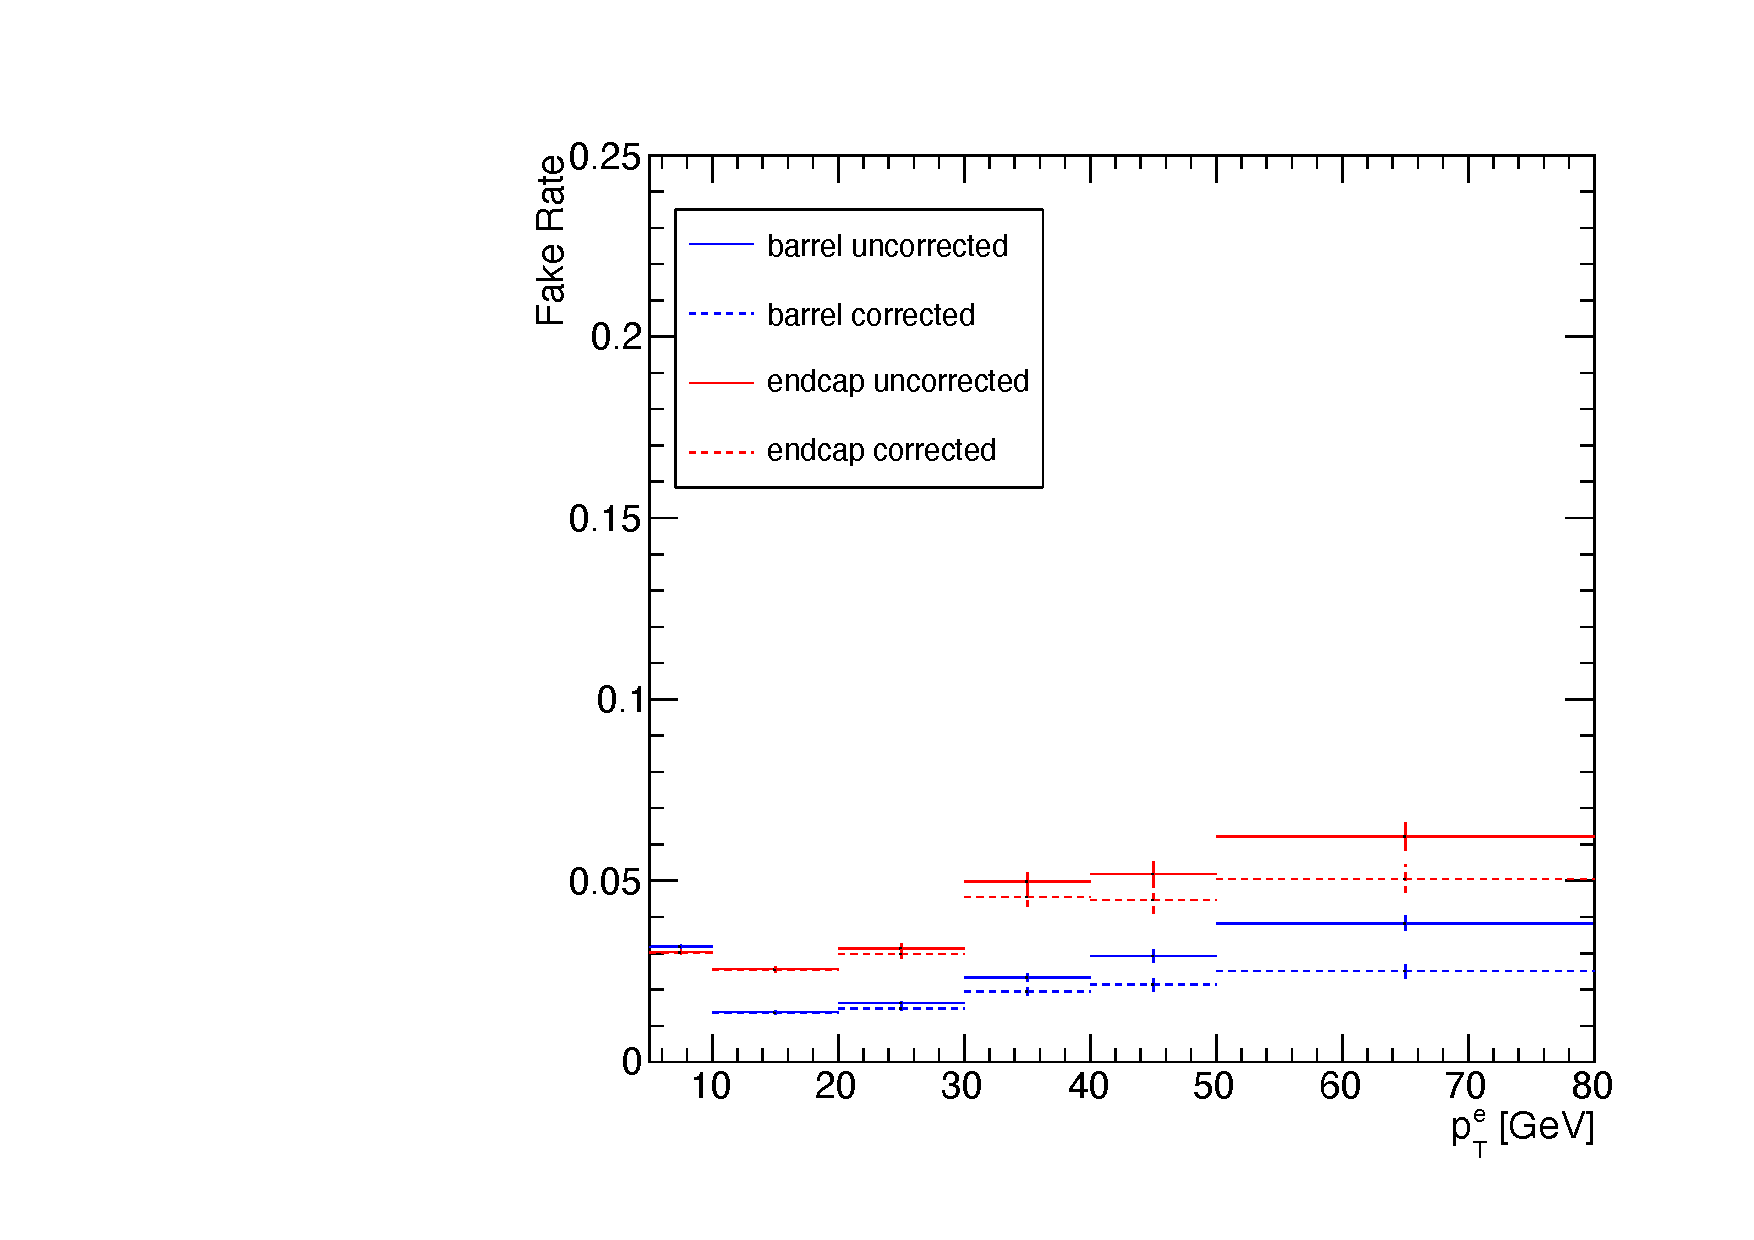
\includegraphics[width=0.48\textwidth]{figures/higgsmassmeas/redbkg/fr/fakerates_UL2017_el_yaxis_full.pdf}
		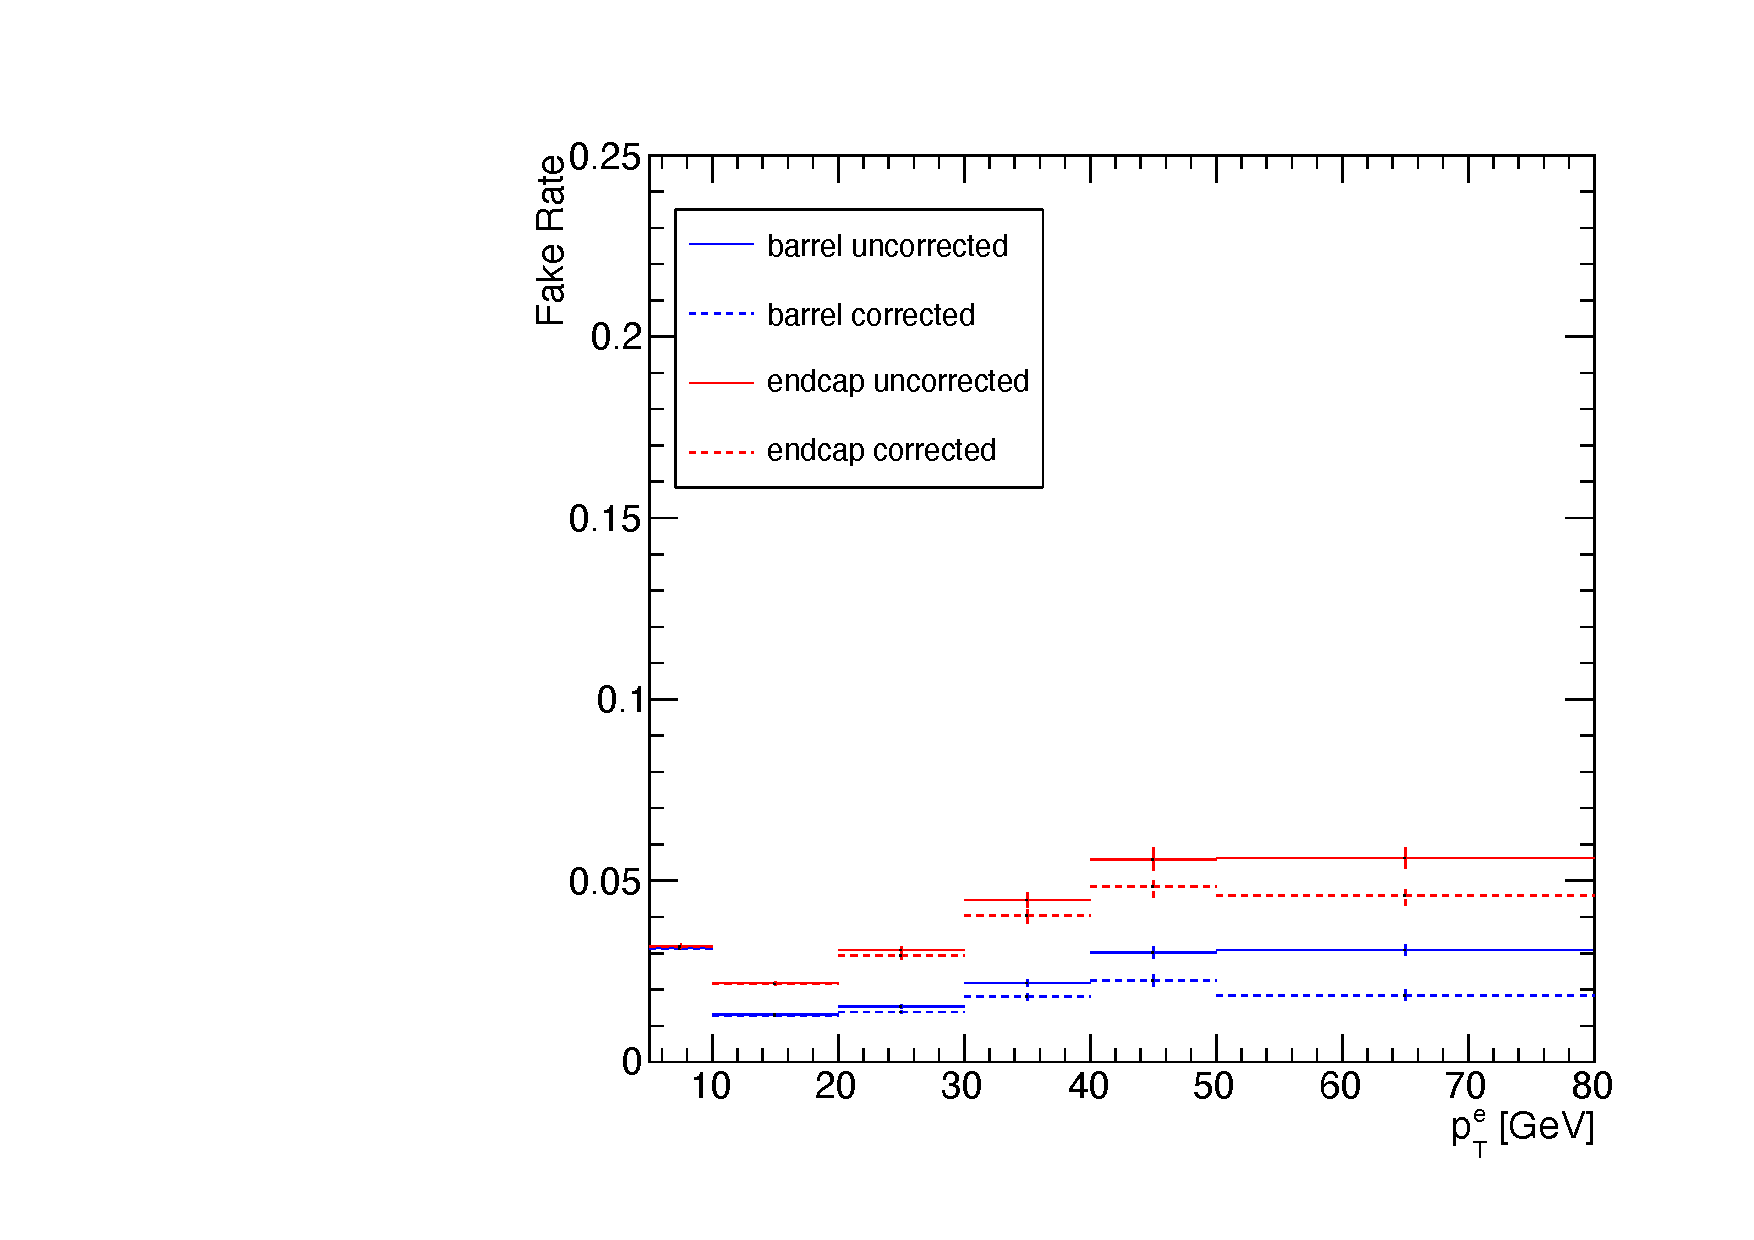
\includegraphics[width=0.48\textwidth]{figures/higgsmassmeas/redbkg/fr/fakerates_UL2018_el_yaxis_full.pdf}
		\caption{
			Electron misidentification rates \vs the \pt of the probe electron evaluated for the OS Method selecting $\PZ + \Pe$ events in UL data
			for each year in Run 2:
			2016 pre-VFP (top left),
			2016 post-VFP (top right),
			2017 (bottom left), and
			2018 (bottom right).
			Rates are evaluated separately for the barrel (blue lines) and endcap (red lines) regions,
			partitioned at $\abs{\eta^{\Pe}} = 1.497$.
			The final rates (dashed lines) are calculated by subtracting out the expected \WZ contribution---estimated from simulation---from the numerator and denominator in the rate calculation.
		}
		\label{fr_plots_el}
	\end{center}
\end{figure}
\begin{figure}[!htbp]
	\begin{center}
		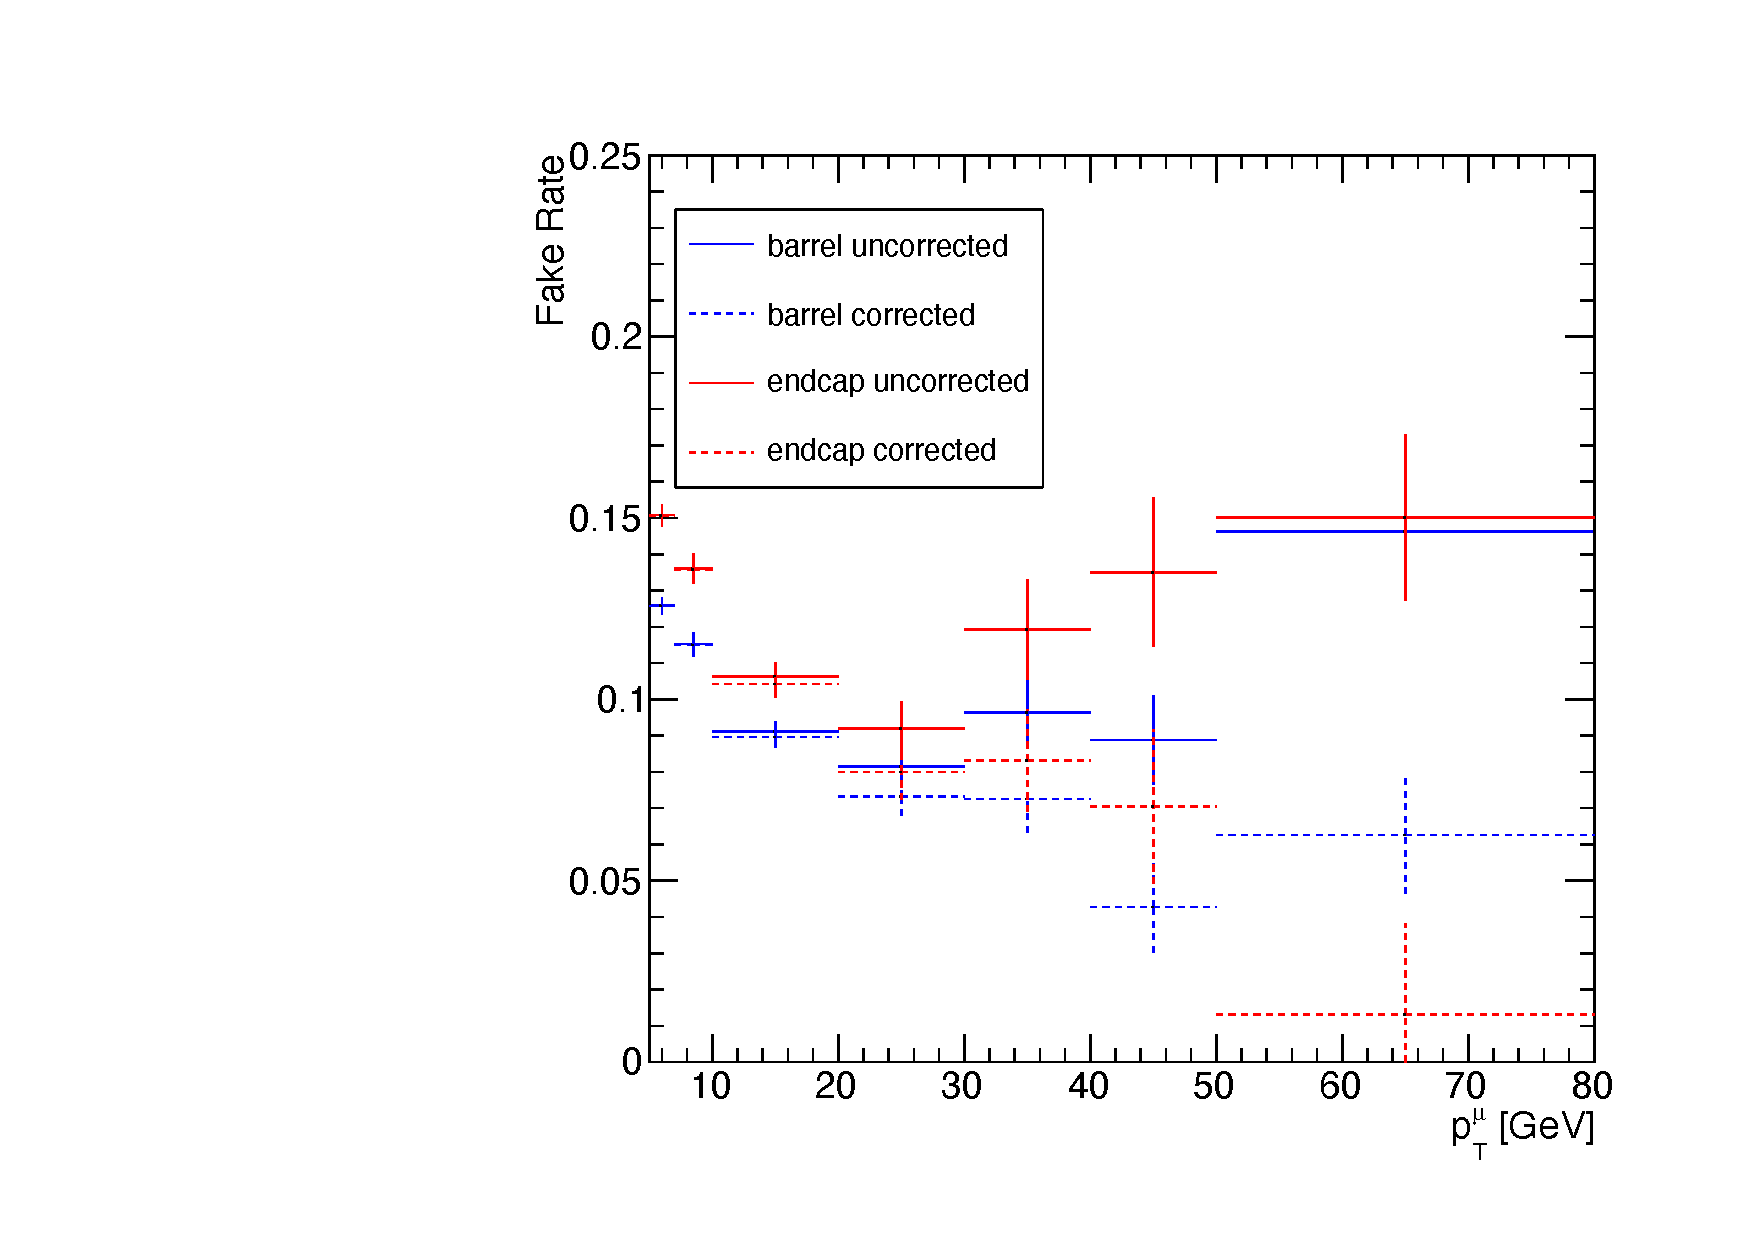
\includegraphics[width=0.48\textwidth]{figures/higgsmassmeas/redbkg/fr/fakerates_UL2016preVFP_mu_yaxis_full.pdf}
		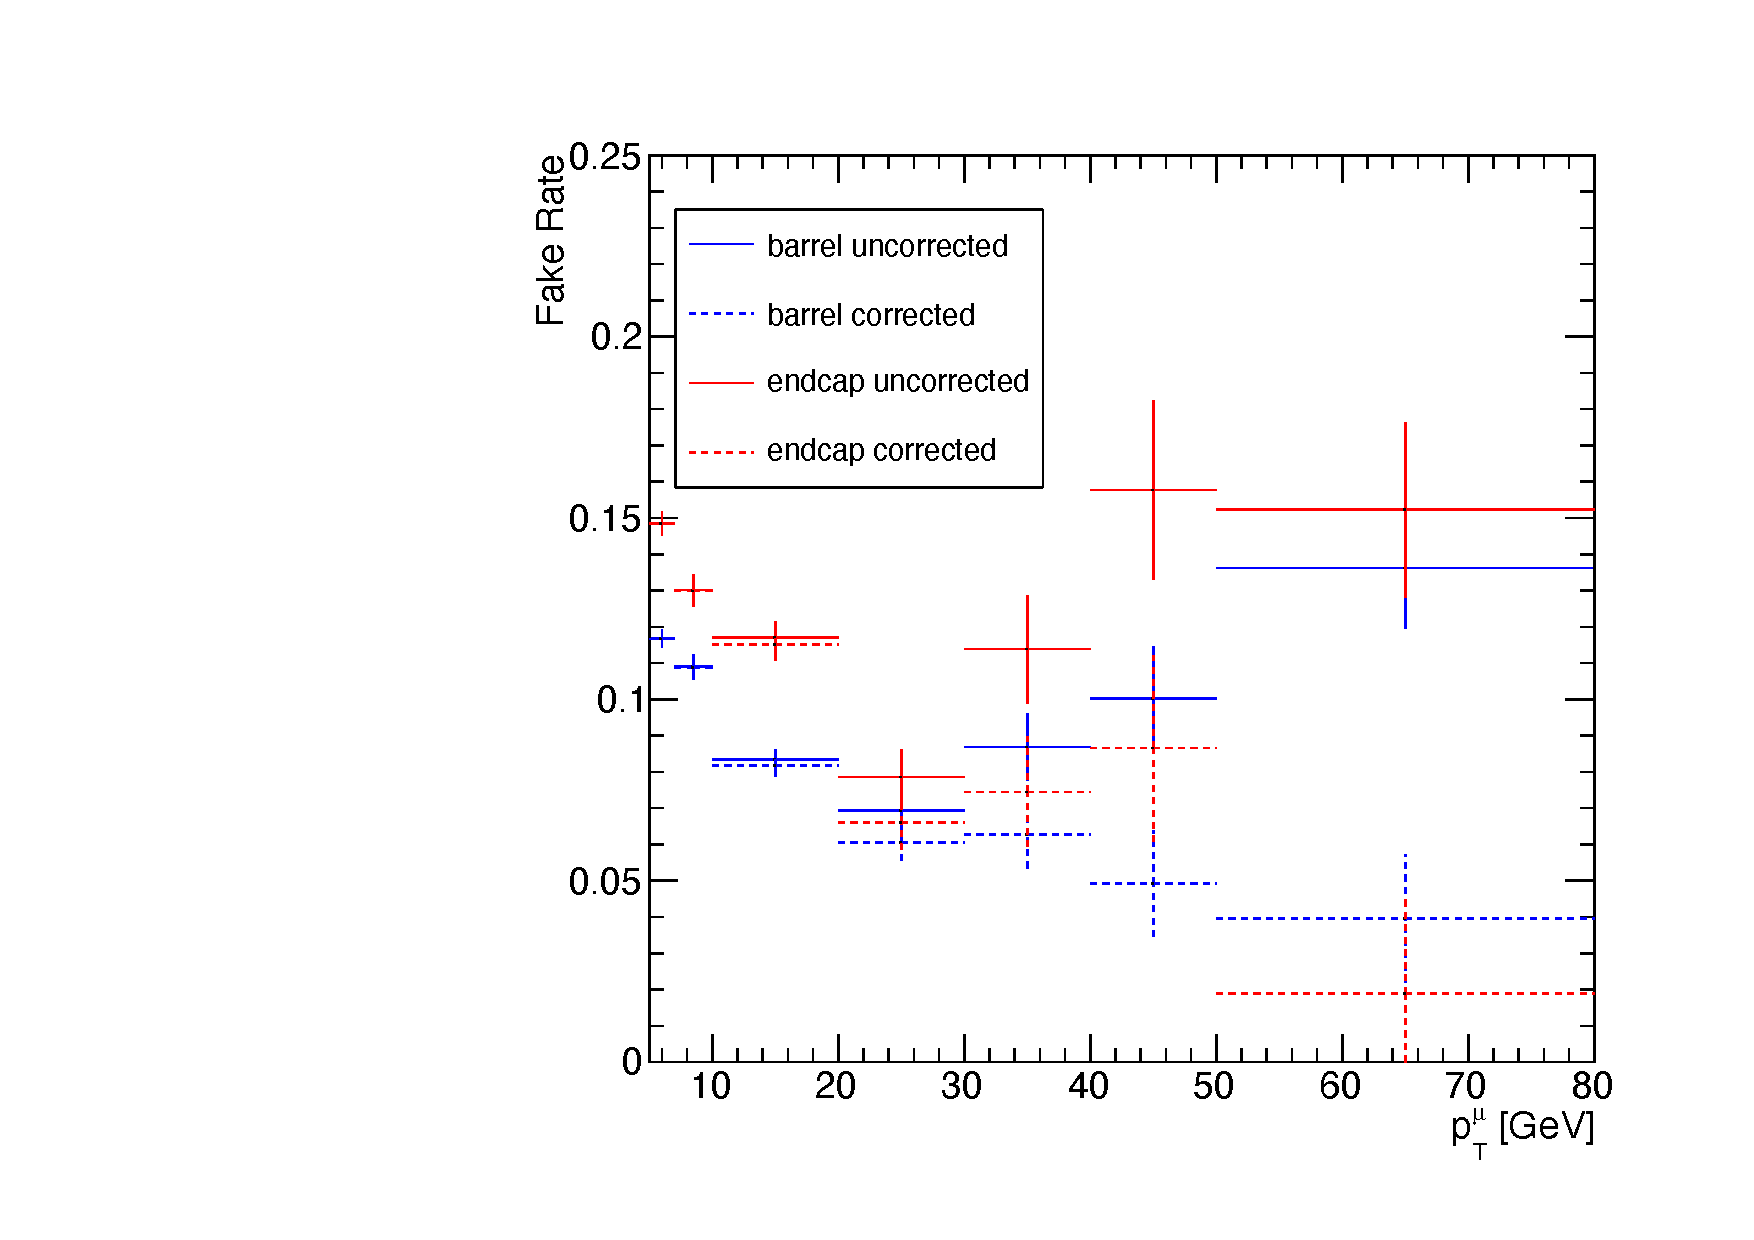
\includegraphics[width=0.48\textwidth]{figures/higgsmassmeas/redbkg/fr/fakerates_UL2016postVFP_mu_yaxis_full.pdf}
		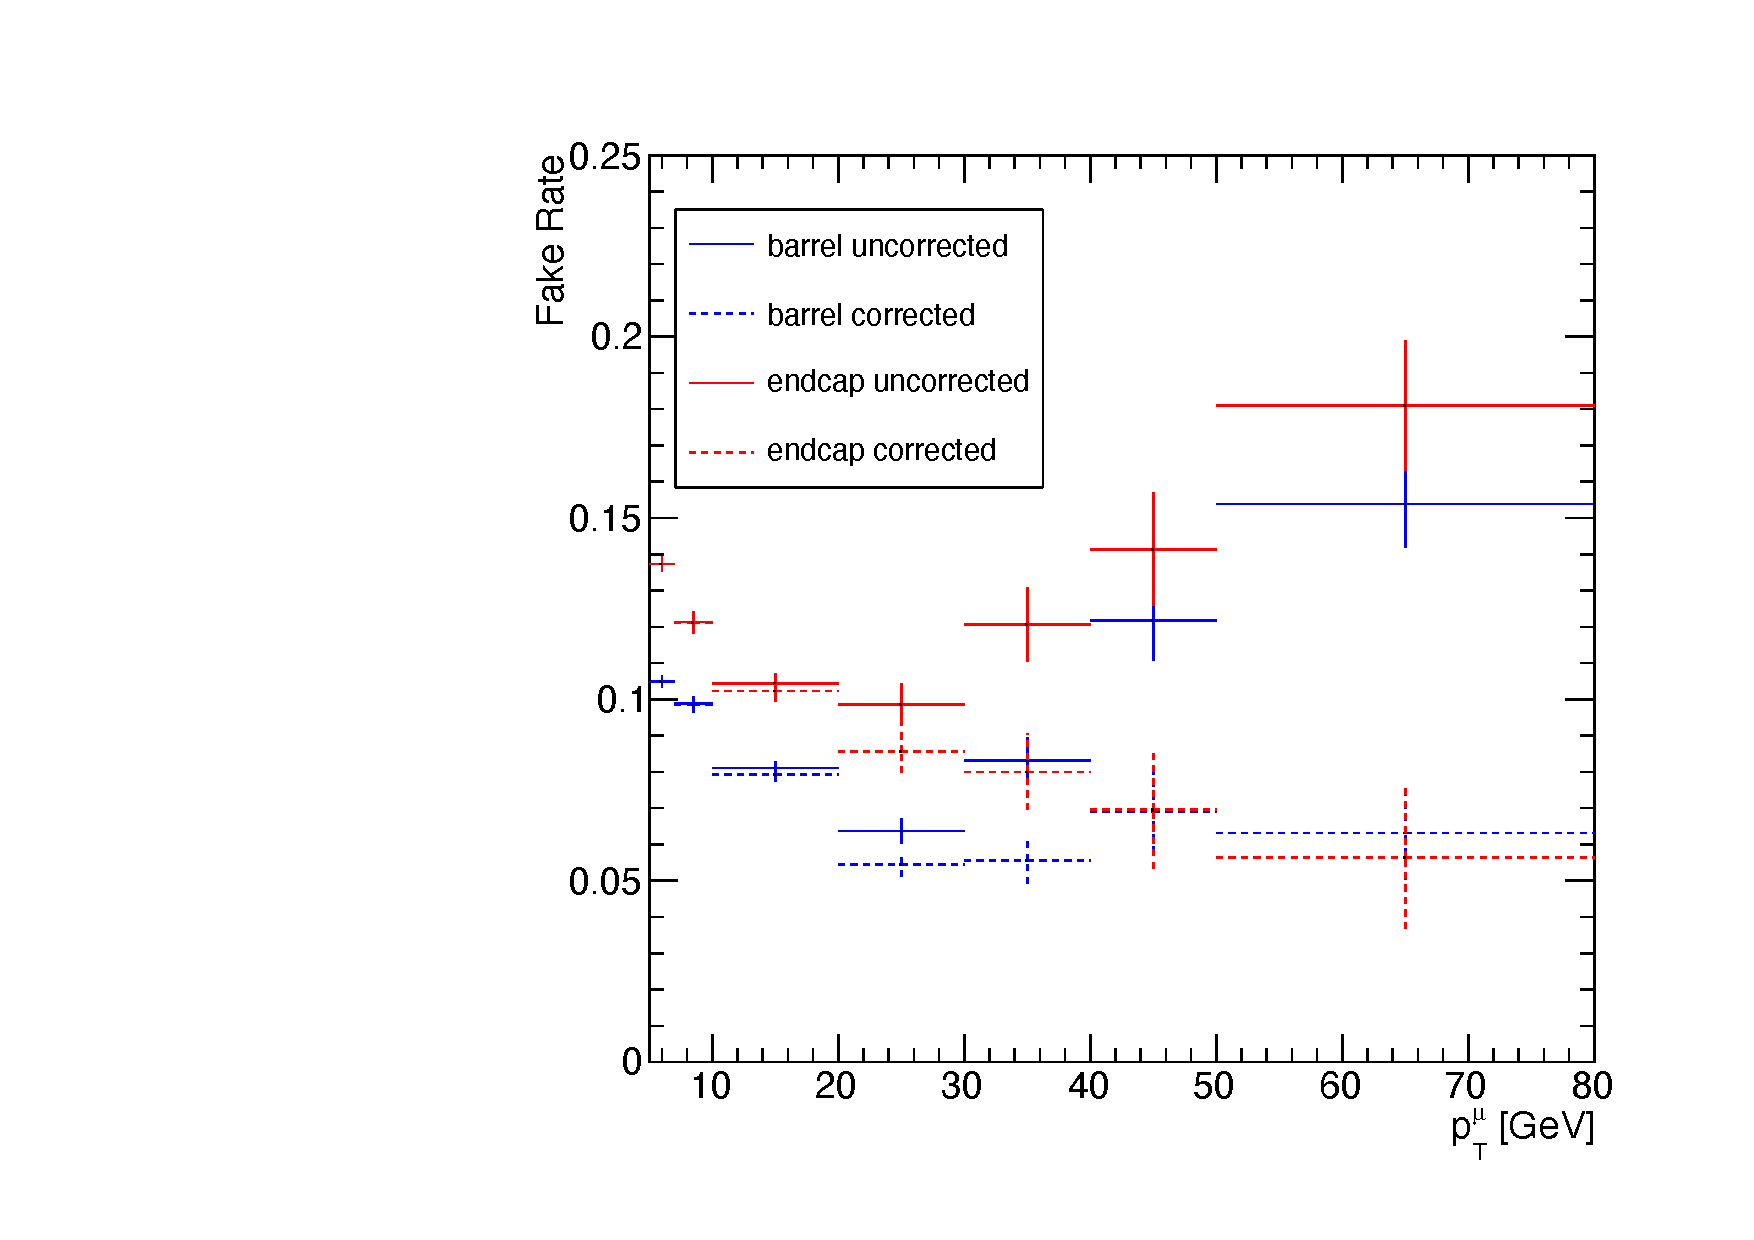
\includegraphics[width=0.48\textwidth]{figures/higgsmassmeas/redbkg/fr/fakerates_UL2017_mu_yaxis_full.pdf}
		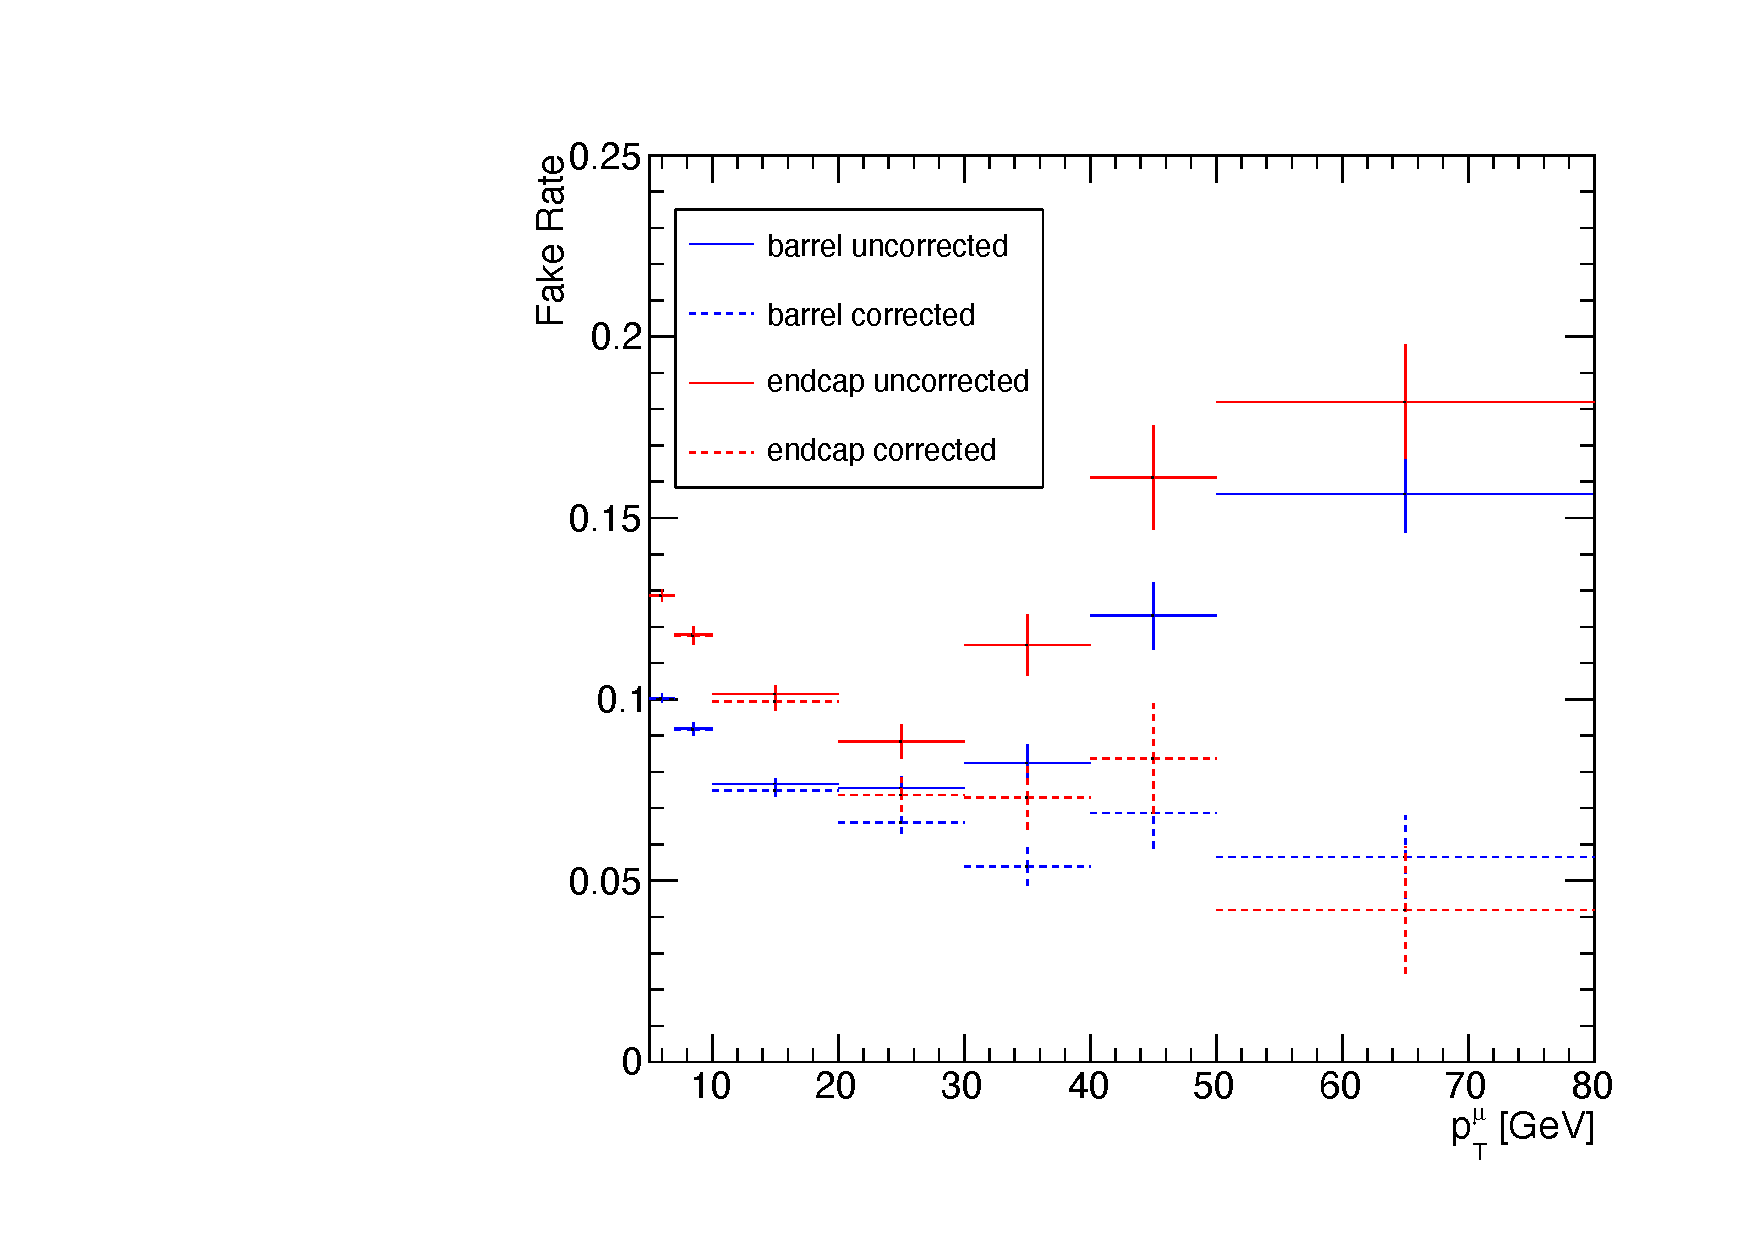
\includegraphics[width=0.48\textwidth]{figures/higgsmassmeas/redbkg/fr/fakerates_UL2018_mu_yaxis_full.pdf}
		\caption{
			Muon misidentification rates \vs the \pt of the probe muon evaluated for the OS Method selecting $\PZ + \mu$ events in UL data
			for each year in Run 2:
			2016 pre-VFP (top left),
			2016 post-VFP (top right),
			2017 (bottom left), and
			2018 (bottom right).
			Rates are evaluated separately for the barrel (blue lines) and endcap (red lines) regions,
			partitioned at $\abs{\eta^{\mu}} = 1.2$.
			The final rates (dashed lines) are calculated by subtracting out the expected \WZ contribution---estimated from simulation---from the numerator and denominator in the rate calculation.
		}
		\label{fr_plots_mu}
	\end{center}
\end{figure}
% \subsubsection{OS Method event selection}
% \label{osmethod_evtsel}
